\DocumentMetadata{%
 %  uncompress, %only for debugging!!
  pdfversion=2.0,
  testphase={phase-II, tabular, graphic}%
 % testphase={phase-II,math, tabular, graphic}% TOC Does not work
   % testphase={phase-III,math}% TOC works
}
\tagpdfsetup{activate, tabsorder=structure}
% Use the following to fix bug in November 2023 download of LaTeX
\ExplSyntaxOn
\cs_generate_variant:Nn\__tag_prop_gput:Nnn{cnx}
\ExplSyntaxOff
\documentclass[11pt,
  english,
  letterpaper,
]{article}
\usepackage{sa4ss}
\usepackage{amsmath,amssymb,array}
\usepackage{booktabs}

% From tagged-template.latex
\usepackage{lmodern}
\usepackage{ifxetex,ifluatex}
\ifnum 0\ifxetex 1\fi\ifluatex 1\fi=0 % if pdftex
  \usepackage[T1]{fontenc}
  \usepackage[utf8]{inputenc}
  \usepackage{textcomp} % provide euro and other symbols
\else % if luatex or xetex
  \usepackage{unicode-math}
  \defaultfontfeatures{Scale=MatchLowercase}
  \defaultfontfeatures[\rmfamily]{Ligatures=TeX,Scale=1}
\fi

% Use upquote if available, for straight quotes in verbatim environments
\IfFileExists{upquote.sty}{\usepackage{upquote}}{}
\IfFileExists{microtype.sty}{% use microtype if available
  \usepackage[]{microtype}
  \UseMicrotypeSet[protrusion]{basicmath} % disable protrusion for tt fonts
}{}
\makeatletter
\@ifundefined{KOMAClassName}{% if non-KOMA class
  \IfFileExists{parskip.sty}{%
    \usepackage{parskip}
  }{% else
    \setlength{\parindent}{0pt}
    \setlength{\parskip}{6pt plus 2pt minus 1pt}}
}{% if KOMA class
  \KOMAoptions{parskip=half}}
\makeatother
\usepackage{xcolor}
\IfFileExists{xurl.sty}{\usepackage{xurl}}{} % add URL line breaks if available
\hypersetup{
  pdftitle={Status of Copper Rockfish (Sebastes caurinus) along the California North of Pt. Conception U.S. West coast in 2022},
  pdflang={en},
  hidelinks,
  pdfcreator={LaTeX via pandoc}}
\urlstyle{same} % disable monospaced font for URLs
\usepackage{longtable}
% Correct order of tables after \paragraph or \subparagraph
\usepackage{etoolbox}
\makeatletter
\patchcmd\longtable{\par}{\if@noskipsec\mbox{}\fi\par}{}{}
\makeatother
% Allow footnotes in longtable head/foot
\IfFileExists{footnotehyper.sty}{\usepackage{footnotehyper}}{\usepackage{footnote}}
\makesavenoteenv{longtable}
\usepackage{graphicx}
\makeatletter
\def\maxwidth{\ifdim\Gin@nat@width>\linewidth\linewidth\else\Gin@nat@width\fi}
\def\maxheight{\ifdim\Gin@nat@height>\textheight\textheight\else\Gin@nat@height\fi}
\makeatother
% Scale images if necessary, so that they will not overflow the page
% margins by default, and it is still possible to overwrite the defaults
% using explicit options in \includegraphics[width, height, ...]{}
\setkeys{Gin}{width=\maxwidth,height=\maxheight,keepaspectratio}
% Set default figure placement to htbp
\makeatletter
\def\fps@figure{htbp}
\makeatother
\setlength{\emergencystretch}{3em} % prevent overfull lines
\providecommand{\tightlist}{%
  \setlength{\itemsep}{0pt}\setlength{\parskip}{0pt}}
\setcounter{secnumdepth}{5}
\ifxetex
  % Load polyglossia as late as possible: uses bidi with RTL langages (e.g. Hebrew, Arabic)
  \usepackage{polyglossia}
  \setmainlanguage[]{}
\else
  \usepackage[shorthands=off,main=english]{babel}
\fi

%Define cslreferences environment, required by pandoc 2.8
%https://github.com/rstudio/rmarkdown/issues/1649
\newlength{\csllabelwidth}
\setlength{\csllabelwidth}{3em}
\newlength{\cslhangindent}
\setlength{\cslhangindent}{1.5em}
% for Pandoc 2.8 to 2.10.1
\newenvironment{cslreferences}%
  {}%
  {\par}
% For Pandoc 2.11+
\newenvironment{CSLReferences}[2] % #1 hanging-ident, #2 entry spacing
 {% don't indent paragraphs
  \setlength{\parindent}{0pt}
  % turn on hanging indent if param 1 is 1
  \ifodd #1 \everypar{\setlength{\hangindent}{\cslhangindent}}\ignorespaces\fi
  % set entry spacing
  \ifnum #2 > 0
  \setlength{\parskip}{#2\baselineskip}
  \fi
 }%
 {}
\usepackage{calc}  % for \widthof, \maxof in minipage
\newcommand{\CSLBlock}[1]{#1\hfill\break}
\newcommand{\CSLLeftMargin}[1]{\parbox[t]{\csllabelwidth}{#1}}
\newcommand{\CSLRightInline}[1]{\parbox[t]{\linewidth - \csllabelwidth}{#1}\break}
\newcommand{\CSLIndent}[1]{\hspace{\cslhangindent}#1}


\providecommand{\tightlist}{%
  \setlength{\itemsep}{0pt}\setlength{\parskip}{0pt}}


\date{}
\newcommand{\trTitle}{Status of Copper Rockfish (\emph{Sebastes caurinus}) along the California North of Pt. Conception U.S. West coast in 2022}
\newcommand{\trYear}{2023}
\newcommand{\trMonth}{April}
\newcommand{\trAuthsLong}{truetruetrue}
\newcommand{\trAuthsBack}{Monk, M.H., C.R. Wetzel, J. Coates}
\newcommand{\trCitation}{
\begin{hangparas}{1em}{1}
\trAuthsBack{}. \trYear{}. \trTitle{}. \glsentrylong{pfmc}, Portland, Oregon. \pageref{LastPage}{}\,p.
\end{hangparas}}

\newcommand\includegraphicsifexists[2][width=\linewidth]{\IfFileExists{#2}{\includegraphics[#1]{#2}}{}}

\begin{document}

%%%%% Frontmatter %%%%%

% Footnote symbols in front matter
\renewcommand*{\thefootnote}{\fnsymbol{footnote}}

\small
\thispagestyle{empty}
\pagenumbering{roman}
\noindent
\begin{center}
\title{Status of Copper Rockfish (\emph{Sebastes caurinus}) along the California North of Pt. Conception U.S. West coast in 2022}
% \textnormal{\MakeTextUppercase{\trTitle{}}}
\vspace{1.5cm}
{\Large\textbf\newline{Status of Copper Rockfish (\emph{Sebastes caurinus}) along the California North of Pt. Conception U.S. West coast in 2022}}

\includegraphicsifexists[width=4in]{figure_title.png}
\vfill
by\\
Melissa H. Monk\textsuperscript{1}\\
Chantel R. Wetzel\textsuperscript{2}\\
Julia Coates\textsuperscript{3}\vfill
\textsuperscript{1}Southwest Fisheries Science Center, U.S. Department of Commerce, National Oceanic and Atmospheric Administration, National Marine Fisheries Service, 110 McAllister Way, Santa Cruz, California 95060\\
\textsuperscript{2}Northwest Fisheries Science Center, U.S. Department of Commerce, National Oceanic and Atmospheric Administration, National Marine Fisheries Service, 2725 Montlake Boulevard East, Seattle, Washington 98112\\
\textsuperscript{3}.na.character\vfill
\trMonth{} \trYear{}
\end{center}
\clearpage

% Fourth page: Colophon
\thispagestyle{empty}
\vspace*{\fill}
\begin{center}
\copyright{} \glsentrylong{pfmc}, \trYear{}\\
\end{center}
\par
\bigskip
\noindent
Correct citation for this publication:
\bigskip
\par
\trCitation{}
\clearpage

% Add TOC to pdf bookmarks (clickable pdf)
\pdfbookmark[1]{\contentsname}{toc}

% Table of contents page, lists of figures and tables
\tableofcontents\clearpage
\label{TRlastRoman}
\clearpage

% Table of contents
\newpage
\thispagestyle{empty} % to remove page number

% Settings for the main document
\pagenumbering{arabic}  % Regular page numbers
\pagestyle{plain}  % No page number on first page of main document, use 'empty'
\renewcommand*{\thefootnote}{\arabic{footnote}}  % Back to numeric footnotes
\setcounter{footnote}{0}  % And start at 1
\renewcommand{\headrulewidth}{0.5pt}
\renewcommand{\footrulewidth}{0.5pt}
%\pagestyle{fancy}\fancyhead[c]{Draft: Do not cite or circulate}

\newcommand{\lt}{\ensuremath <}
\newcommand{\gt}{\ensuremath >}

\pagebreak
\pagenumbering{roman}
\setcounter{page}{1}

\renewcommand{\thetable}{\roman{table}}
\renewcommand{\thefigure}{\roman{figure}}

\setlength\parskip{0.5em plus 0.1em minus 0.2em}

\hypertarget{executive-summary}{%
\section*{Executive summary}\label{executive-summary}}
\addcontentsline{toc}{section}{Executive summary}

\hypertarget{stock}{%
\subsection*{Stock}\label{stock}}
\addcontentsline{toc}{subsection}{Stock}

This assessment reports the status of copper rockfish (\emph{Sebastes caurinus}) off the California coast in U.S. waters, using data through 2022. The copper rockfish stock was assessed using two sub-area models that captured distinct inter-stock dynamics split north and south of Point Conception. The estimated dynamics for each assessed sub-area is described here along with the combined stock status for the California stock. This assessment does not account for populations located in Mexico waters or other areas off the U.S. coast and assumes that these southern and northern populations do not contribute to the population being assessed here.

\hypertarget{catches}{%
\subsection*{Catches}\label{catches}}
\addcontentsline{toc}{subsection}{Catches}

Replace text with trends and current levels. Include Table for last 10 years. Include Figure with long-term estimates.

\begingroup\fontsize{10}{12}\selectfont
\begingroup\fontsize{10}{12}\selectfont

\begin{longtable}[t]{r>{\centering\arraybackslash}p{1.83cm}>{\centering\arraybackslash}p{1.83cm}>{\centering\arraybackslash}p{1.83cm}>{\centering\arraybackslash}p{1.83cm}>{\centering\arraybackslash}p{1.83cm}}
\caption{\label{tab:south-removalsES}Recent catch by fleet and total catch summed across fleets for the sub-area model south of Point Conception.}\\
\toprule
Year & Commercial dead & Commercial live & Rec CPFV & Rec Private & Total Catch\\
\midrule
\endfirsthead
\caption[]{Recent catch by fleet and total catch summed across fleets for the sub-area model south of Point Conception. \textit{(continued)}}\\
\toprule
Year & Commercial dead & Commercial live & Rec CPFV & Rec Private & Total Catch\\
\midrule
\endhead

\endfoot
\bottomrule
\endlastfoot
2013 & 1.26 & 2.67 & 61.65 & 13.96 & 79.54\\
2014 & 1.79 & 2.29 & 47.58 & 10.04 & 61.71\\
2015 & 2.11 & 4.09 & 67.00 & 8.97 & 82.18\\
2016 & 2.11 & 3.57 & 82.20 & 11.07 & 98.95\\
2017 & 1.74 & 2.82 & 70.58 & 11.72 & 86.86\\
2018 & 2.93 & 2.20 & 81.97 & 14.21 & 101.31\\
2019 & 2.71 & 3.08 & 60.25 & 14.66 & 80.70\\
2020 & 3.54 & 3.58 & 56.39 & 23.01 & 86.52\\
2021 & 2.74 & 1.94 & 44.25 & 8.28 & 57.20\\
2022 & 0.69 & 0.21 & 14.12 & 4.50 & 19.52\\*
\end{longtable}
\endgroup{}
\endgroup{}


\begingroup\fontsize{10}{12}\selectfont
\begingroup\fontsize{10}{12}\selectfont

\begin{table}[t]{r>{\centering\arraybackslash}p{1.83cm}>{\centering\arraybackslash}p{1.83cm}>{\centering\arraybackslash}p{1.83cm}>{\centering\arraybackslash}p{1.83cm}>{\centering\arraybackslash}p{1.83cm}}
\caption{\label{tab:north-removalsES}Recent catches (mt) by fleet and total catch (mt) summed across fleets for the sub-area model north of Point Conception.}\\
\toprule
Year & Commercial Dead & Commercial Live & Rec CPFV & Rec PR & Total Catch\\
\midrule
\endfirsthead
\caption[]{Recent catches (mt) by fleet and total catch (mt) summed across fleets for the sub-area model north of Point Conception. \textit{(continued)}}\\
\toprule
Year & Commercial Dead & Commercial Live & Rec CPFV & Rec PR & Total Catch\\
\midrule
\endhead

\endfoot
\bottomrule
\endlastfoot
2013 & 0.70 & 2.11 & 8.83 & 14.00 & 25.64\\
2014 & 0.74 & 2.47 & 16.10 & 17.63 & 36.94\\
2015 & 0.78 & 2.69 & 24.22 & 37.77 & 65.46\\
2016 & 0.83 & 2.57 & 28.69 & 34.23 & 66.32\\
2017 & 1.41 & 4.60 & 56.48 & 76.13 & 138.62\\
2018 & 3.04 & 6.36 & 43.97 & 49.01 & 102.38\\
2019 & 2.49 & 6.85 & 39.16 & 53.39 & 101.89\\
2020 & 3.90 & 7.55 & 36.55 & 55.17 & 103.17\\
2021 & 3.10 & 7.55 & 24.98 & 41.42 & 77.05\\
2022 & 1.19 & 1.92 & 11.50 & 32.53 & 47.15\\
\end{table}
\endgroup{}
\endgroup{}


\begin{figure}
\centering
\includegraphics[width=1\textwidth,height=1\textheight]{S:/copper_rockfish_2023/models/sca/5.5_est_m/plots/catch2 landings stacked.png}
\caption{Landings by fleet used in the base model for the area south of Point Conception where catches in metric tons by fleet are stacked.\label{fig:es-south-catch}}
\end{figure}

\begin{figure}
\centering
\includegraphics[width=1\textwidth,height=1\textheight]{S:/copper_rockfish_2023/models/nca/8.5_update_deb_index/plots/catch2 landings stacked.png}
\caption{Landings by fleet used in the base model for the area north of Point Conception where catches in metric tons by fleet are stacked.\label{fig:es-north-catch}}
\end{figure}

\hypertarget{data-and-assessment}{%
\subsection*{Data and assessment}\label{data-and-assessment}}
\addcontentsline{toc}{subsection}{Data and assessment}

This assessment uses the stock assessment framework Stock Synthesis version 3.30.21 (SS3).

Replace text with date of last assessment, type of assessment model, data available, new information, and information lacking.

\hypertarget{stock-biomass-and-dynamics}{%
\subsection*{Stock biomass and dynamics}\label{stock-biomass-and-dynamics}}
\addcontentsline{toc}{subsection}{Stock biomass and dynamics}

Replace text with trends and current levels relative to virgin or historic levels and description of uncertainty. Include Table for last 10 years. Include Figure with long-term estimates.

\begingroup\fontsize{10}{12}\selectfont
\begingroup\fontsize{10}{12}\selectfont

\begin{longtable}[t]{r>{\centering\arraybackslash}p{1.57cm}>{\centering\arraybackslash}p{1.57cm}>{\centering\arraybackslash}p{1.57cm}>{\centering\arraybackslash}p{1.57cm}>{\centering\arraybackslash}p{1.57cm}>{\centering\arraybackslash}p{1.57cm}}
\caption{\label{tab:south-ssbES}Estimated recent trend in spawning output and the fraction unfished and the 95 percent intervals for the sub-area model south of Point Conception.}\\
\toprule
Year & Spawning Output & Lower Interval & Upper Interval & Fraction Unfished & Lower Interval & Upper Interval\\
\midrule
\endfirsthead
\caption[]{Estimated recent trend in spawning output and the fraction unfished and the 95 percent intervals for the sub-area model south of Point Conception. \textit{(continued)}}\\
\toprule
Year & Spawning Output & Lower Interval & Upper Interval & Fraction Unfished & Lower Interval & Upper Interval\\
\midrule
\endhead

\endfoot
\bottomrule
\endlastfoot
2013 & 29.22 & 21.10 & 37.34 & 0.14 & 0.10 & 0.19\\
2014 & 30.05 & 21.41 & 38.69 & 0.15 & 0.10 & 0.20\\
2015 & 33.46 & 23.92 & 43.00 & 0.17 & 0.11 & 0.22\\
2016 & 36.13 & 25.51 & 46.75 & 0.18 & 0.12 & 0.24\\
2017 & 37.56 & 25.74 & 49.38 & 0.19 & 0.12 & 0.25\\
2018 & 39.23 & 26.06 & 52.40 & 0.19 & 0.12 & 0.26\\
2019 & 37.92 & 23.46 & 52.38 & 0.19 & 0.11 & 0.26\\
2020 & 35.69 & 20.06 & 51.32 & 0.18 & 0.10 & 0.26\\
2021 & 32.45 & 15.87 & 49.03 & 0.16 & 0.08 & 0.24\\
2022 & 30.24 & 12.91 & 47.57 & 0.15 & 0.06 & 0.24\\
2023 & 29.76 & 11.87 & 47.65 & 0.15 & 0.06 & 0.24\\*
\end{longtable}
\endgroup{}
\endgroup{}


\begingroup\fontsize{10}{12}\selectfont
\begingroup\fontsize{10}{12}\selectfont

\begin{longtable}[t]{r>{\centering\arraybackslash}p{1.57cm}>{\centering\arraybackslash}p{1.57cm}>{\centering\arraybackslash}p{1.57cm}>{\centering\arraybackslash}p{1.57cm}>{\centering\arraybackslash}p{1.57cm}>{\centering\arraybackslash}p{1.57cm}}
\caption{\label{tab:north-ssbES}Estimated recent trend in spawning output and the fraction unfished and the 95 percent intervals for the sub-area model north of Point Conception.}\\
\toprule
Year & Spawning Output & Lower Interval & Upper Interval & Fraction Unfished & Lower Interval & Upper Interval\\
\midrule
\endfirsthead
\caption[]{Estimated recent trend in spawning output and the fraction unfished and the 95 percent intervals for the sub-area model north of Point Conception. \textit{(continued)}}\\
\toprule
Year & Spawning Output & Lower Interval & Upper Interval & Fraction Unfished & Lower Interval & Upper Interval\\
\midrule
\endhead

\endfoot
\bottomrule
\endlastfoot
2013 & 170.30 & 94.03  & 246.57 & 0.36 & 0.24 & 0.48\\
2014 & 181.67 & 100.89 & 262.44 & 0.38 & 0.25 & 0.51\\
2015 & 194.73 & 108.27 & 281.19 & 0.41 & 0.27 & 0.55\\
2016 & 205.67 & 113.14 & 298.19 & 0.43 & 0.29 & 0.58\\
2017 & 215.64 & 117.05 & 314.23 & 0.45 & 0.30 & 0.61\\
2018 & 217.87 & 113.23 & 322.51 & 0.46 & 0.29 & 0.63\\
2019 & 223.06 & 112.30 & 333.82 & 0.47 & 0.29 & 0.65\\
2020 & 227.81 & 111.02 & 344.59 & 0.48 & 0.29 & 0.67\\
2021 & 231.68 & 109.06 & 354.31 & 0.49 & 0.29 & 0.69\\
2022 & 237.18 & 108.72 & 365.64 & 0.50 & 0.29 & 0.71\\
2023 & 246.82 & 112.22 & 381.43 & 0.52 & 0.30 & 0.74\\*
\end{longtable}
\endgroup{}
\endgroup{}


\begingroup\fontsize{10}{12}\selectfont
\begingroup\fontsize{10}{12}\selectfont

\begin{longtable}[t]{c>{\centering\arraybackslash}p{2cm}>{\centering\arraybackslash}p{2cm}}
\caption{\label{tab:ca-status}The estimated spawning ouput in number of million eggs across California and fraction unfished by year.}\\
\toprule
Year & Spawning Output & Fraction Unfished\\
\midrule
\endfirsthead
\caption[]{\label{tab:ca-status}The estimated spawning ouput in number of million eggs across California and fraction unfished by year. \textit{(continued)}}\\
\toprule
Year & Spawning Output & Fraction Unfished\\
\midrule
\endhead

\endfoot
\bottomrule
\endlastfoot
2013 & 227.72 & 0.331\\
2014 & 243.57 & 0.354\\
2015 & 264.67 & 0.384\\
2016 & 283.21 & 0.411\\
2017 & 299.59 & 0.435\\
2018 & 308.56 & 0.448\\
2019 & 316.83 & 0.460\\
2020 & 322.83 & 0.469\\
2021 & 319.07 & 0.463\\
2022 & 320.42 & 0.465\\
2023 & 331.05 & 0.481\\*
\end{longtable}
\endgroup{}
\endgroup{}

\begin{figure}
\centering
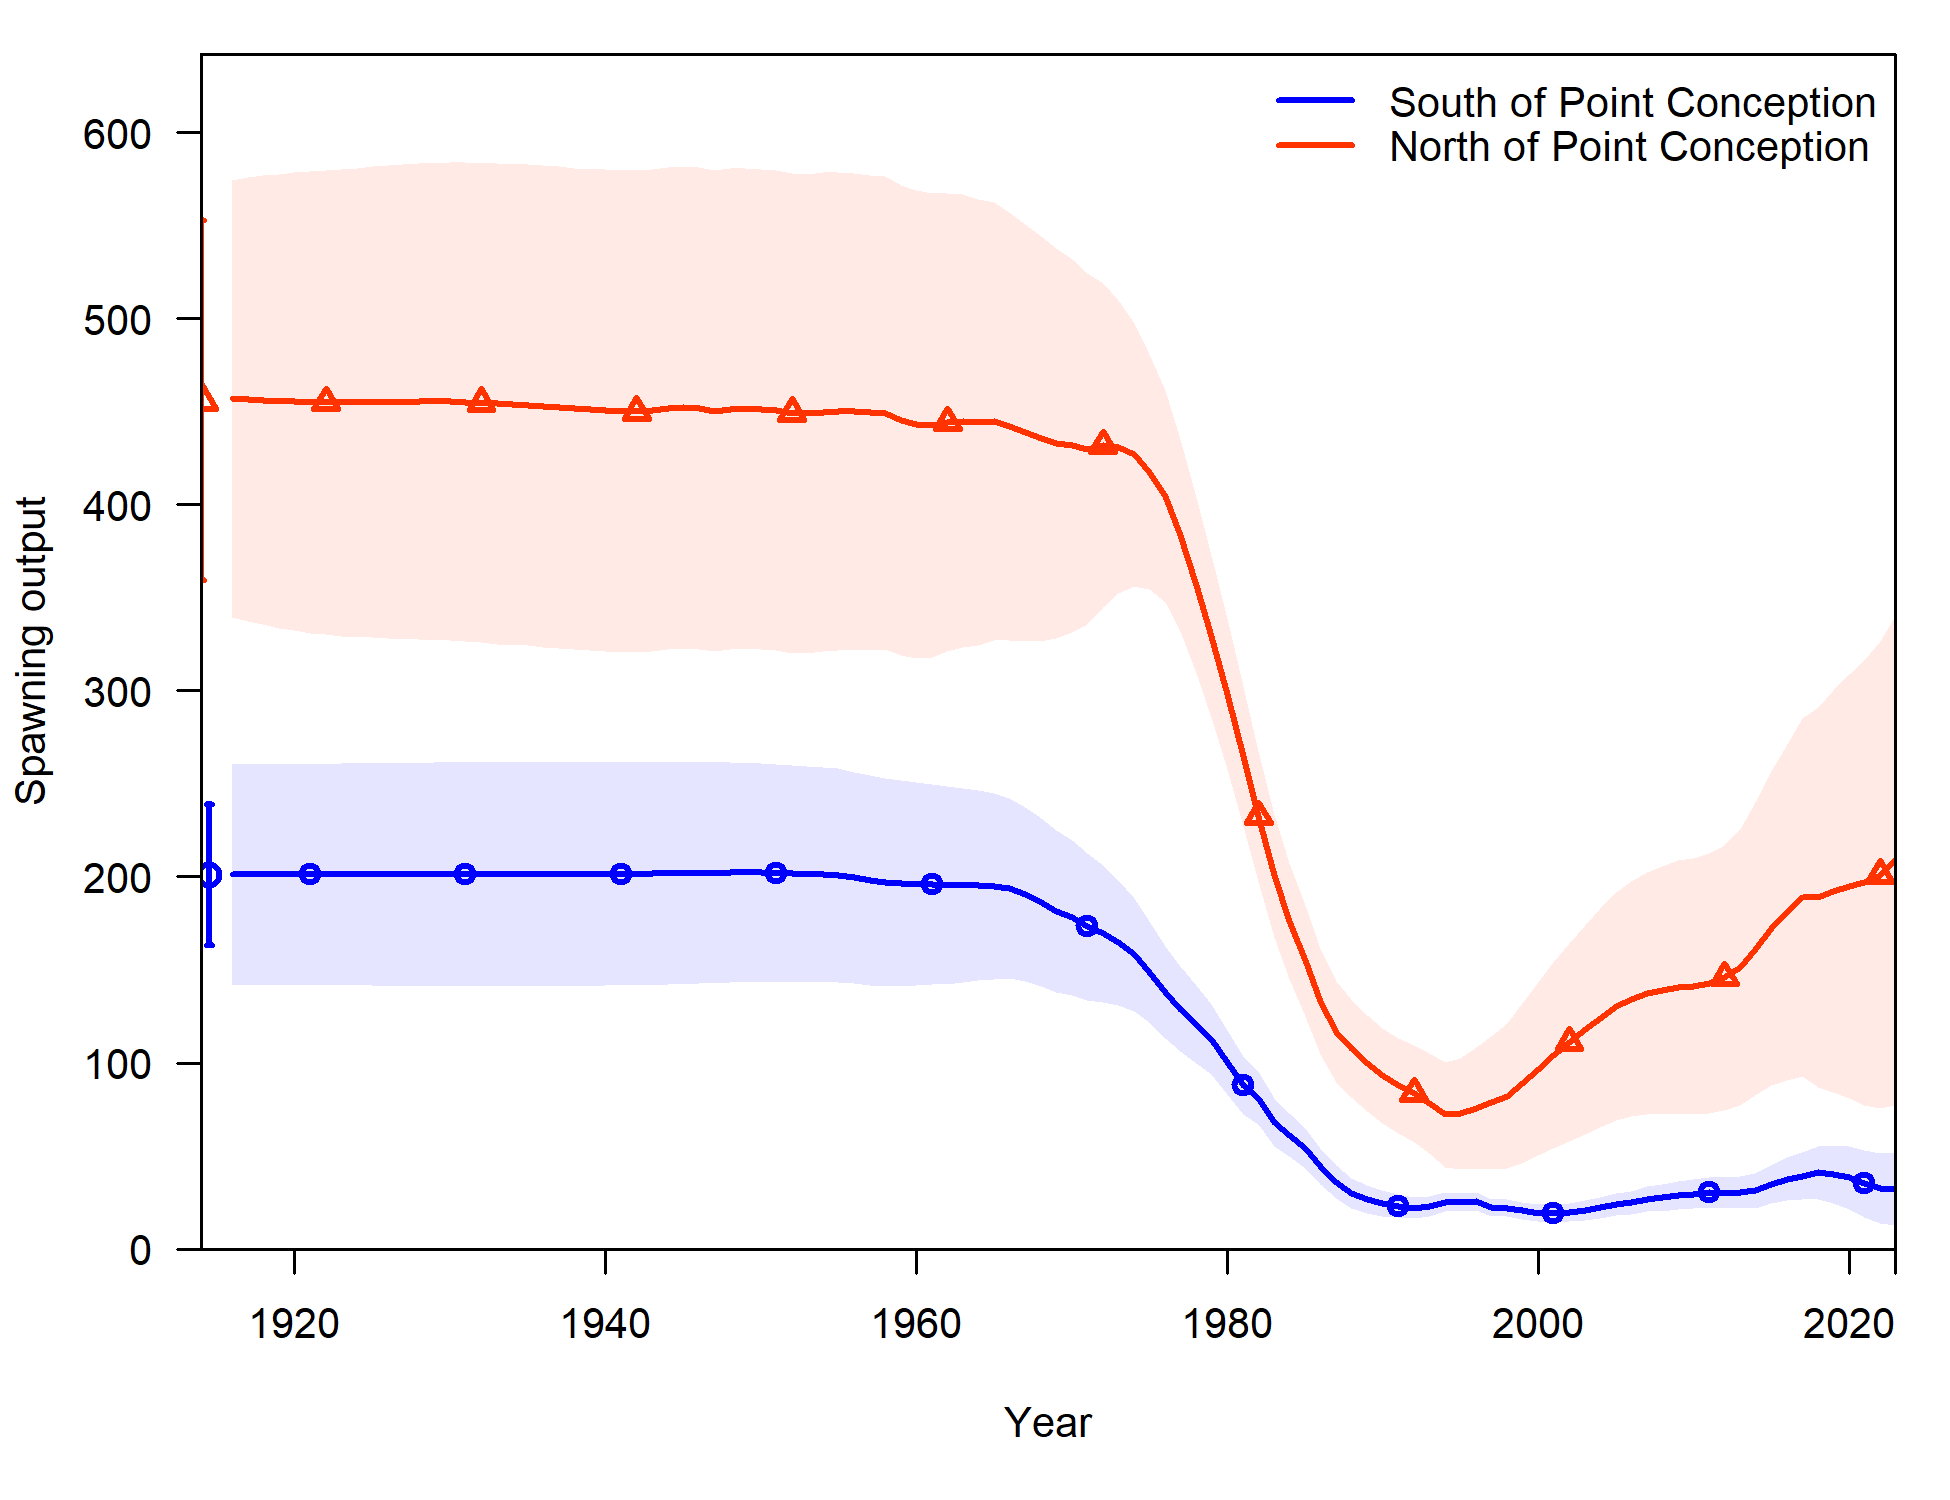
\includegraphics[width=1\textwidth,height=1\textheight]{C:/Users/melissa.monk/Documents/GitHub/copper_rockfish_2023/documents/shared_figures/compare2_spawnbio_uncertainty.png}
\caption{Estimated time series of spawning output (circles and line: median; light broken lines: 95 percent intervals) for the model areas south and north of Point Conception.\label{fig:es-sb}}
\end{figure}

\begin{figure}
\centering
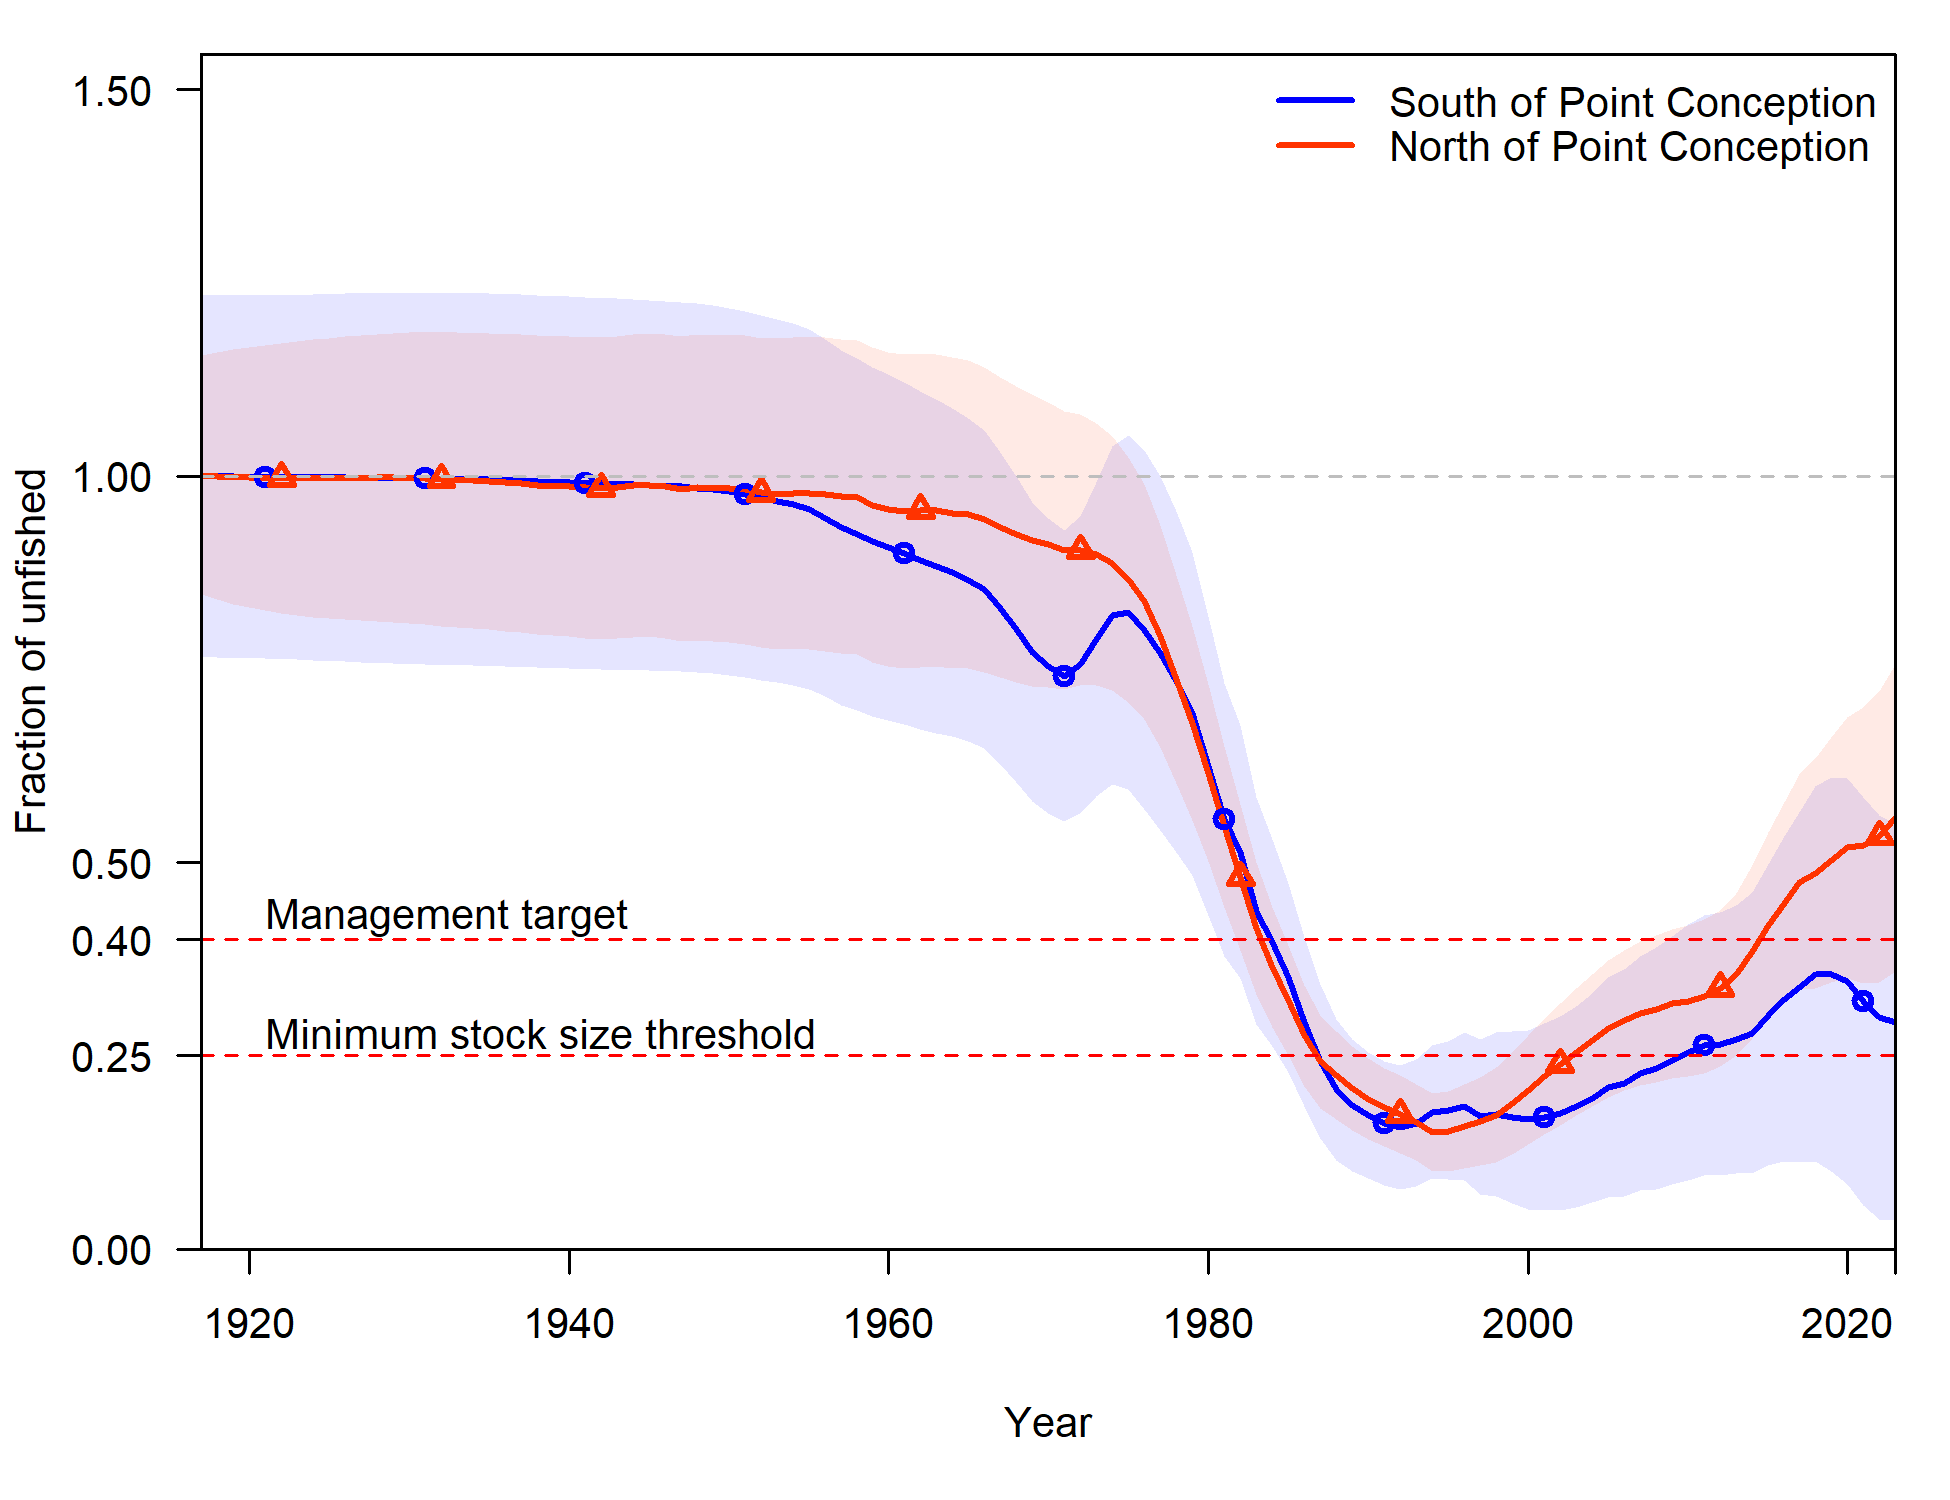
\includegraphics[width=1\textwidth,height=1\textheight]{C:/Users/melissa.monk/Documents/GitHub/copper_rockfish_2023/documents/shared_figures/compare4_Bratio_uncertainty.png}
\caption{Estimated time series of fraction of unfished spawning output (circles and line: median; light broken lines: 95 percent intervals) for the model areas south and north of Point Conception.\label{fig:es-depl}}
\end{figure}

\clearpage

\hypertarget{recruitment}{%
\subsection*{Recruitment}\label{recruitment}}
\addcontentsline{toc}{subsection}{Recruitment}

Replace text with trends and current levels relative to virgin or historic levels and description of uncertainty. Include Table for last 10 years. Include Figure with long-term estimates.

\begingroup\fontsize{10}{12}\selectfont
\begingroup\fontsize{10}{12}\selectfont

\begin{longtable}[t]{r>{\centering\arraybackslash}p{1.57cm}>{\centering\arraybackslash}p{1.57cm}>{\centering\arraybackslash}p{1.57cm}>{\centering\arraybackslash}p{1.57cm}>{\centering\arraybackslash}p{1.57cm}>{\centering\arraybackslash}p{1.57cm}}
\caption{\label{tab:south-recrES}Estimated recent trend in recruitment and recruitment deviations and the 95 percent intervals for the sub-area model south of Point Conception.}\\
\toprule
Year & Recruitment & Lower Interval & Upper Interval & Recruitment Deviations & Lower Interval & Upper Interval\\
\midrule
\endfirsthead
\caption[]{Estimated recent trend in recruitment and recruitment deviations and the 95 percent intervals for the sub-area model south of Point Conception. \textit{(continued)}}\\
\toprule
Year & Recruitment & Lower Interval & Upper Interval & Recruitment Deviations & Lower Interval & Upper Interval\\
\midrule
\endhead

\endfoot
\bottomrule
\endlastfoot
2013 & 613.62 & 381.00 & 988.26 & 1.18 & 0.94 & 1.41\\
2014 & 168.22 & 86.76 & 326.18 & -0.13 & -0.64 & 0.39\\
2015 & 81.26 & 39.81 & 165.88 & -0.88 & -1.45 & -0.30\\
2016 & 114.55 & 59.49 & 220.57 & -0.55 & -1.00 & -0.09\\
2017 & 91.14 & 44.28 & 187.61 & -0.79 & -1.33 & -0.25\\
2018 & 91.39 & 42.11 & 198.33 & -0.80 & -1.40 & -0.19\\
2019 & 119.56 & 51.10 & 279.76 & -0.53 & -1.24 & 0.18\\
2020 & 119.75 & 43.77 & 327.64 & -0.60 & -1.54 & 0.34\\
2021 & 231.44 & 144.36 & 371.04 & 0.00 & 0.00 & 0.00\\
2022 & 227.42 & 138.88 & 372.42 & 0.00 & 0.00 & 0.00\\
2023 & 226.18 & 137.68 & 371.57 & 0.00 & 0.00 & 0.00\\*
\end{longtable}
\endgroup{}
\endgroup{}


\begingroup\fontsize{10}{12}\selectfont
\begingroup\fontsize{10}{12}\selectfont

\begin{longtable}[t]{r>{\centering\arraybackslash}p{1.57cm}>{\centering\arraybackslash}p{1.57cm}>{\centering\arraybackslash}p{1.57cm}>{\centering\arraybackslash}p{1.57cm}>{\centering\arraybackslash}p{1.57cm}>{\centering\arraybackslash}p{1.57cm}}
\caption{\label{tab:north-recrES}Estimated recent trend in recruitment and recruitment deviations and the 95 percent intervals for the sub-area model north of Point Conception.}\\
\toprule
Year & Recruitment & Lower Interval & Upper Interval & Recruitment Deviations & Lower Interval & Upper Interval\\
\midrule
\endfirsthead
\caption[]{Estimated recent trend in recruitment and recruitment deviations and the 95 percent intervals for the sub-area model north of Point Conception. \textit{(continued)}}\\
\toprule
Year & Recruitment & Lower Interval & Upper Interval & Recruitment Deviations & Lower Interval & Upper Interval\\
\midrule
\endhead

\endfoot
\bottomrule
\endlastfoot
2013 & 556.60 & 282.67 & 1095.99 & 0.23 & -0.38 & 0.84\\
2014 & 466.50 & 233.22 & 933.12 & 0.04 & -0.59 & 0.67\\
2015 & 590.78 & 316.19 & 1103.84 & 0.26 & -0.27 & 0.79\\
2016 & 285.96 & 134.46 & 608.15 & -0.47 & -1.18 & 0.24\\
2017 & 869.76 & 474.53 & 1594.18 & 0.63 & 0.13 & 1.12\\
2018 & 618.32 & 318.82 & 1199.18 & 0.25 & -0.34 & 0.84\\
2019 & 345.34 & 159.74 & 746.57 & -0.37 & -1.11 & 0.37\\
2020 & 502.19 & 394.01 & 640.08 & 0.00 & 0.00 & 0.00\\
2021 & 503.74 & 394.44 & 643.32 & 0.00 & 0.00 & 0.00\\
2022 & 505.86 & 395.70 & 646.68 & 0.00 & 0.00 & 0.00\\
2023 & 509.39 & 398.85 & 650.56 & 0.00 & 0.00 & 0.00\\*
\end{longtable}
\endgroup{}
\endgroup{}


\begin{figure}
\centering
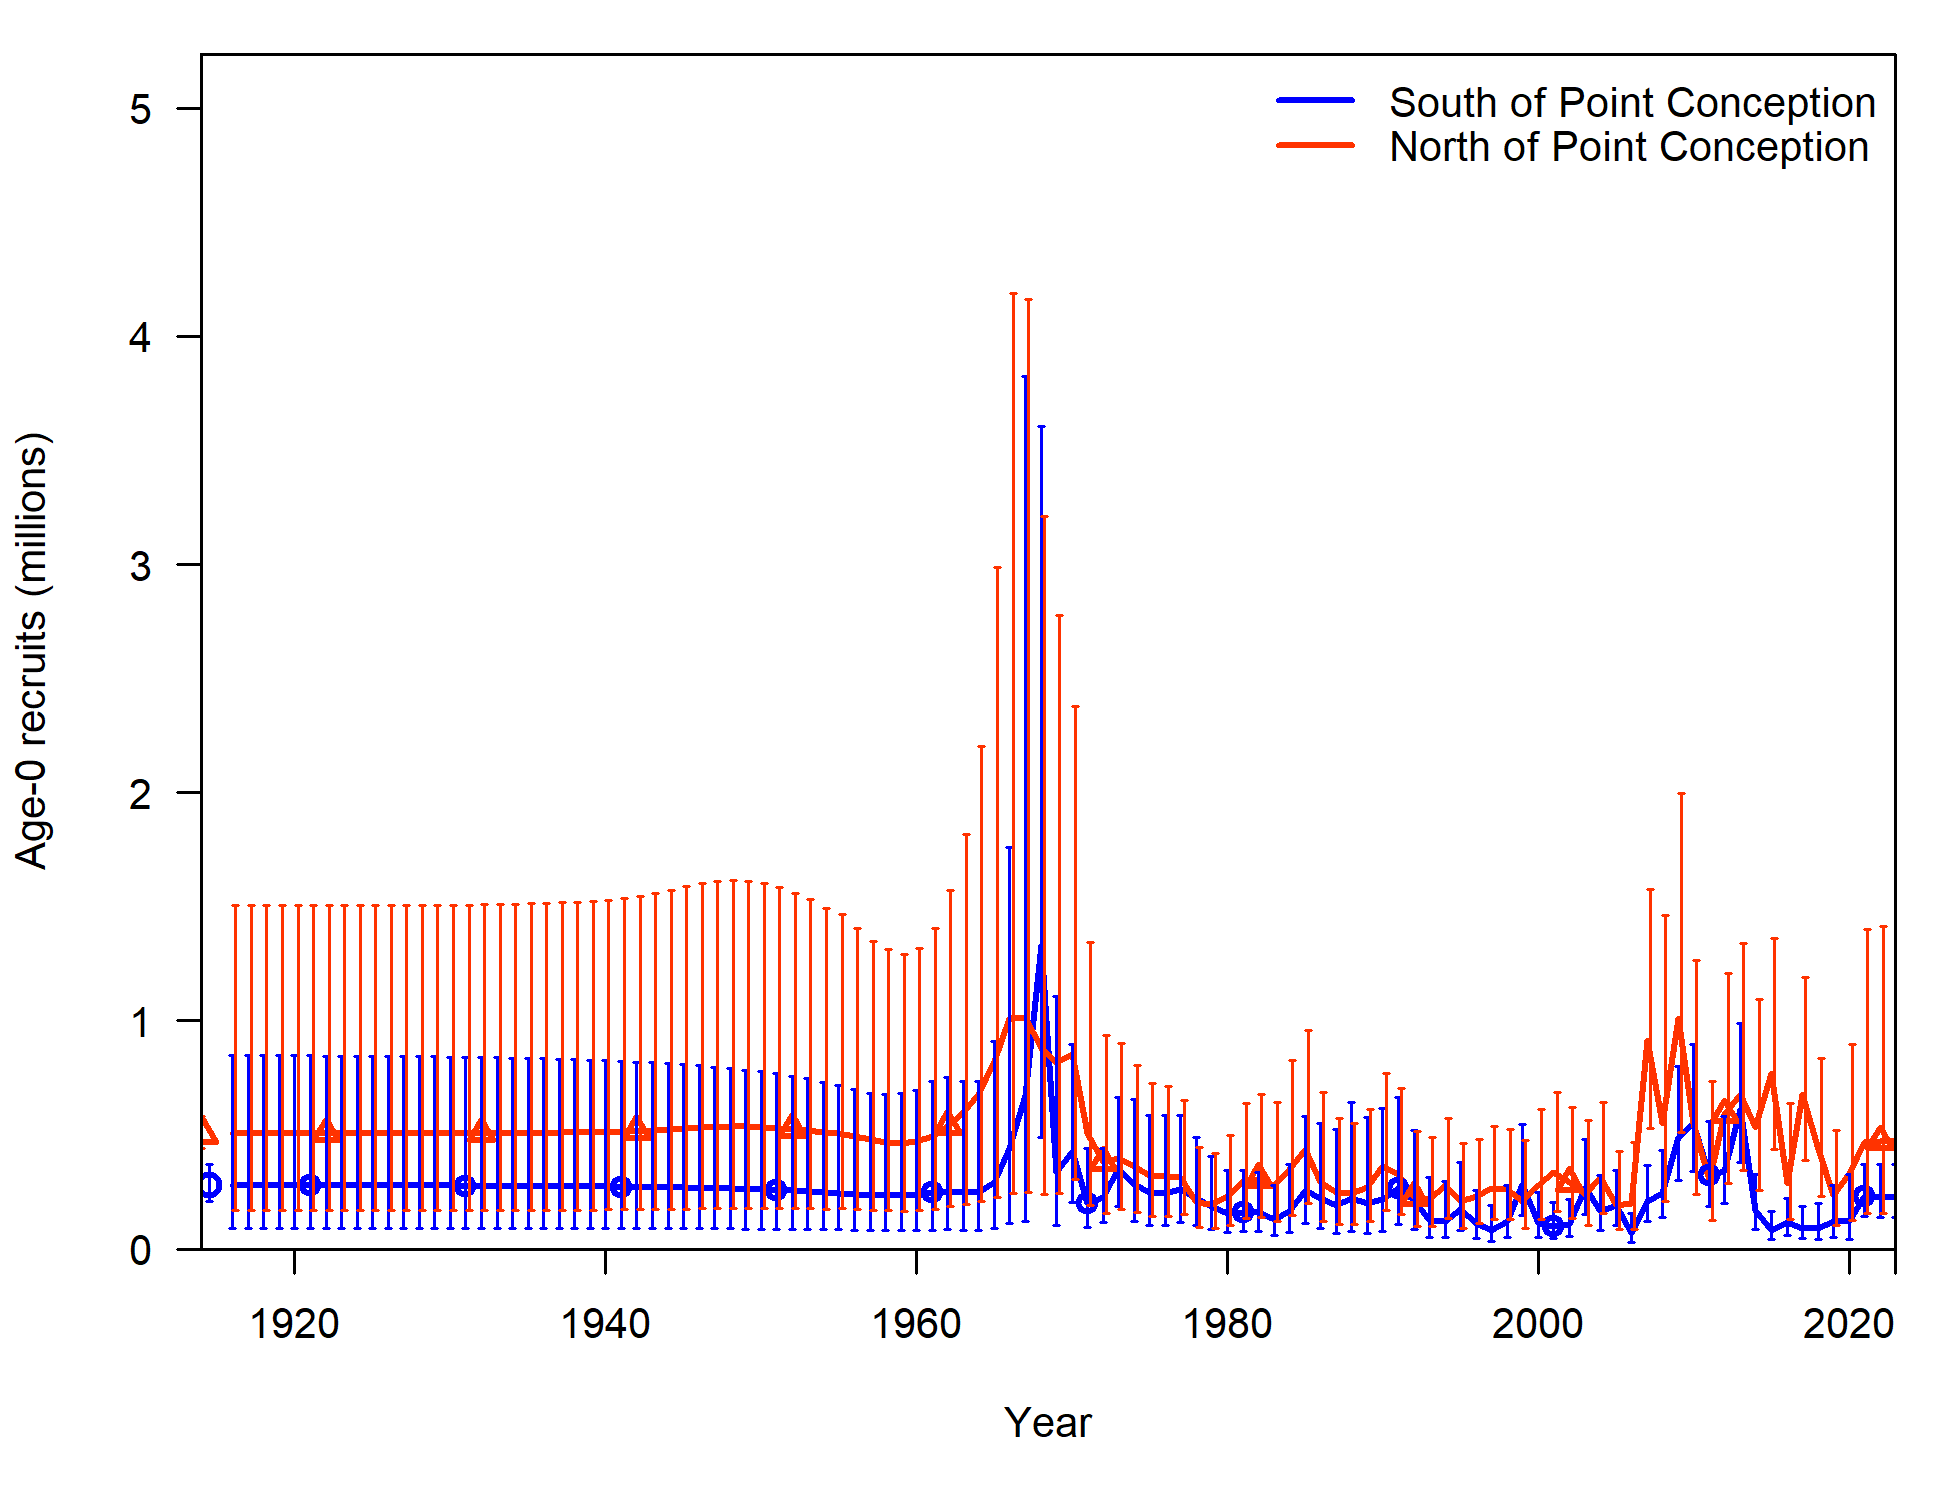
\includegraphics[width=1\textwidth,height=1\textheight]{C:/Users/melissa.monk/Documents/GitHub/copper_rockfish_2023/documents/shared_figures/compare10_recruits_uncertainty.png}
\caption{Estimated time series of age-0 recruits (1000s) for the model areas south and north of Point Conception with 95 percent intervals.\label{fig:es-recruits}}
\end{figure}

\begin{figure}
\centering
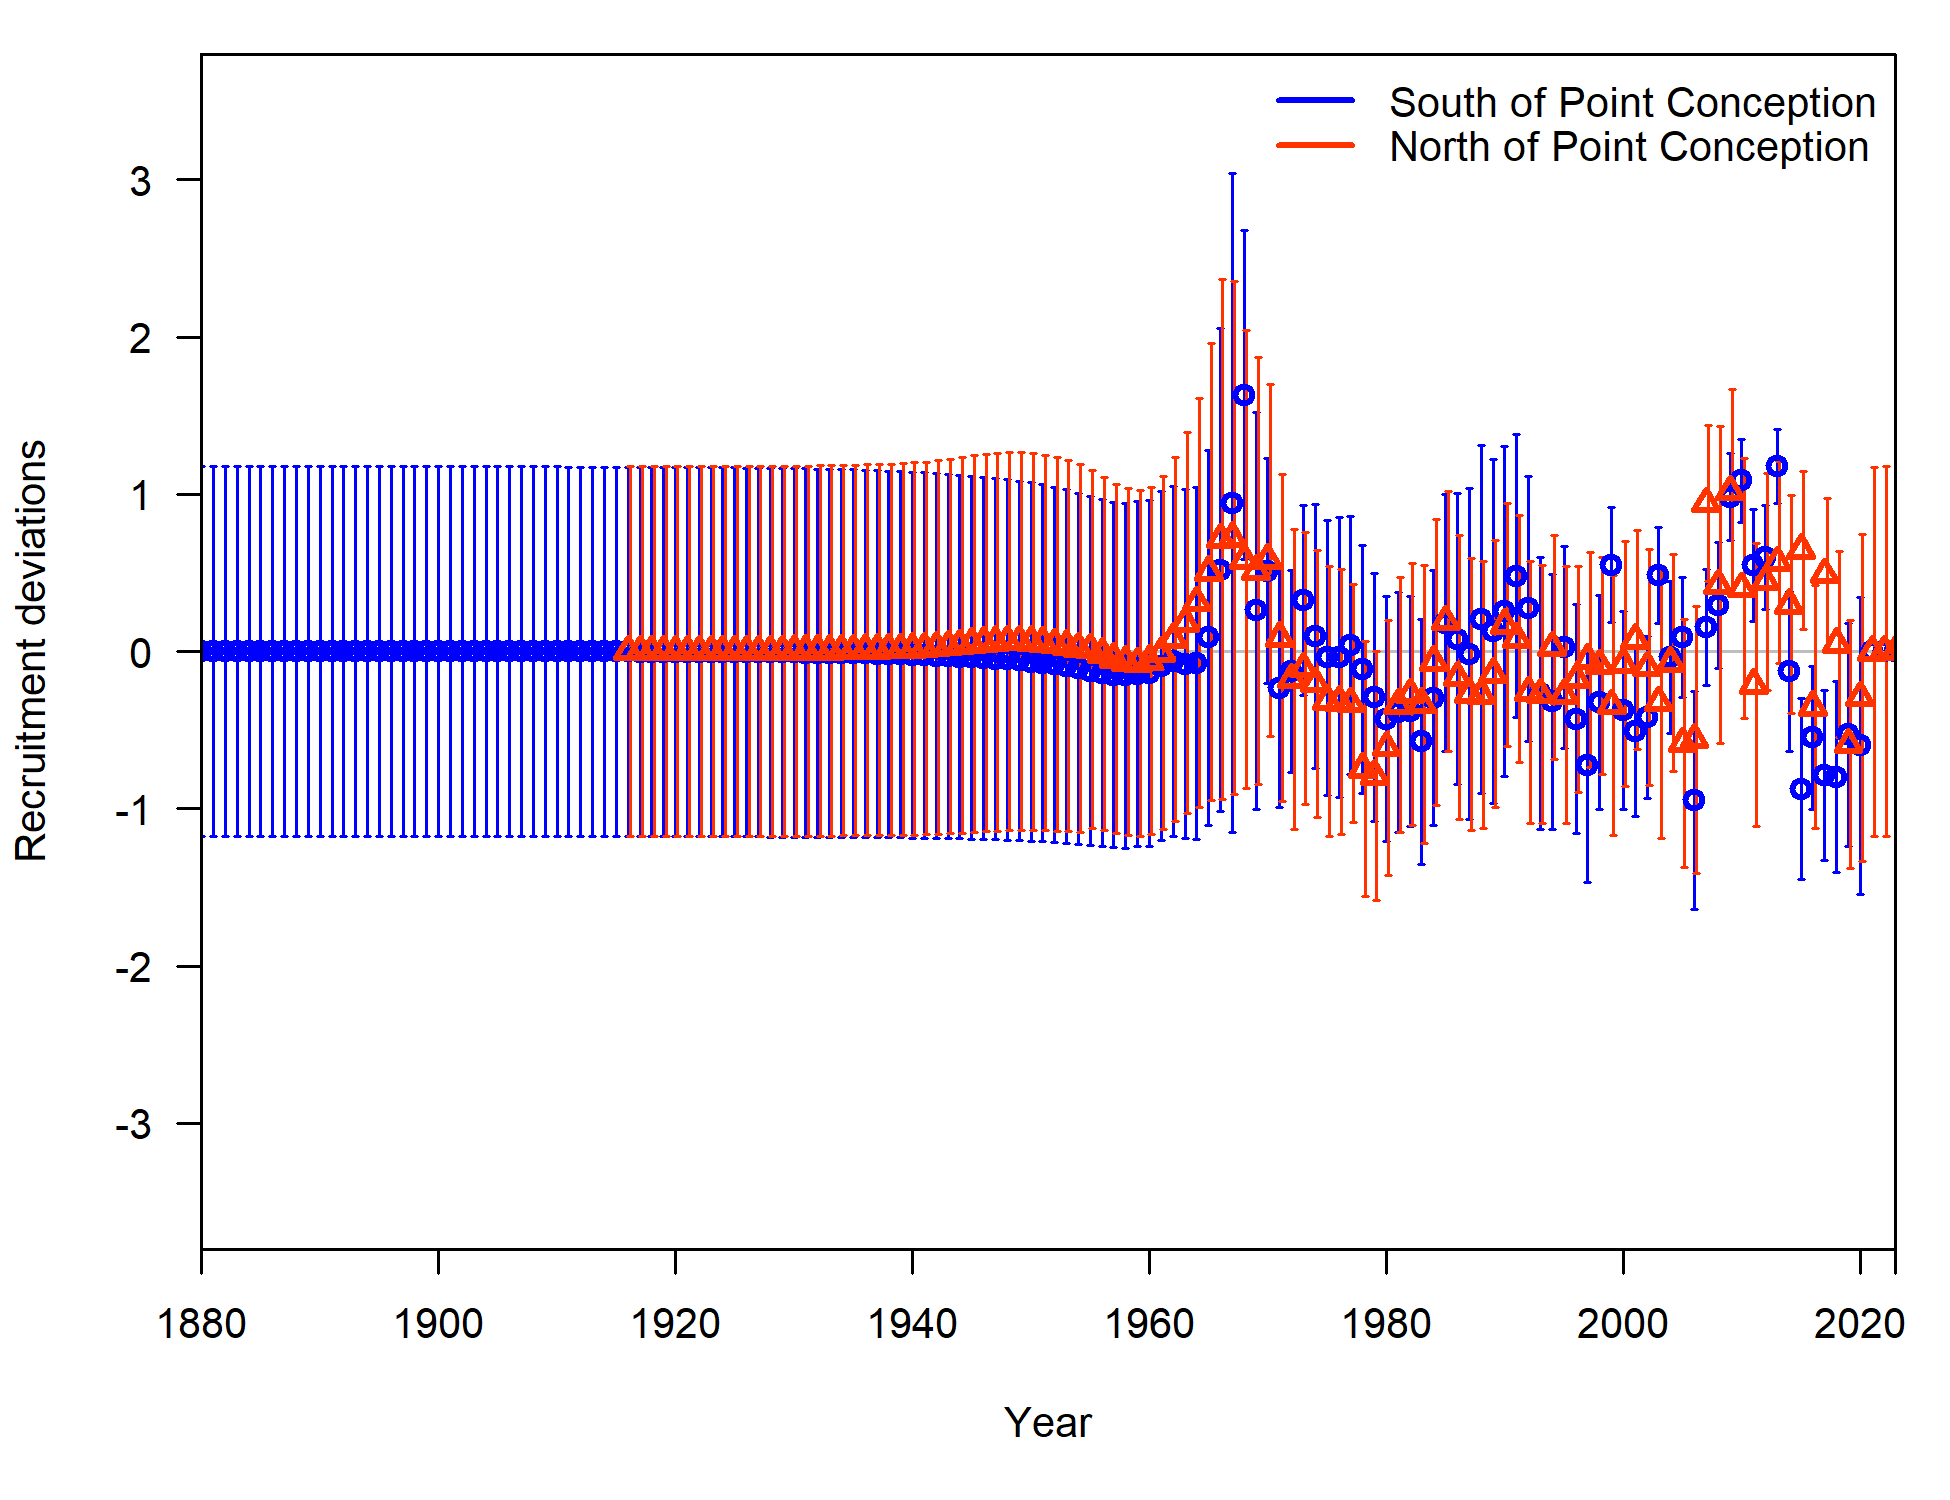
\includegraphics[width=1\textwidth,height=1\textheight]{C:/Users/melissa.monk/Documents/GitHub/copper_rockfish_2023/documents/shared_figures/compare12_recdevs_uncertainty.png}
\caption{Estimated time series of recruitment deviations for the model areas south and north of Point Conception.\label{fig:es-rec-devs}}
\end{figure}

\clearpage

\hypertarget{exploitation-status}{%
\subsection*{Exploitation status}\label{exploitation-status}}
\addcontentsline{toc}{subsection}{Exploitation status}

Replace text with total catch divided by exploitable biomass or SPR harvest rate. Include Table for last 10 years. Include Figure with trend in f relative to target vs.~trend in biomass relative to the target.

\begingroup\fontsize{10}{12}\selectfont
\begingroup\fontsize{10}{12}\selectfont

\begin{longtable}[t]{r>{\centering\arraybackslash}p{1.57cm}>{\centering\arraybackslash}p{1.57cm}>{\centering\arraybackslash}p{1.57cm}>{\centering\arraybackslash}p{1.57cm}>{\centering\arraybackslash}p{1.57cm}>{\centering\arraybackslash}p{1.57cm}}
\caption{\label{tab:south-exploitES}Estimated recent trend in the 1-SPR where SPR is the spawning potential ratio the exploitation rate, and the 95 percent intervals for the sub-area model south of Point Conception.}\\
\toprule
Year & 1-SPR & Lower Interval & Upper Interval & Exploitation Rate & Lower Interval & Upper Interval\\
\midrule
\endfirsthead
\caption[]{Estimated recent trend in the 1-SPR where SPR is the spawning potential ratio the exploitation rate, and the 95 percent intervals for the sub-area model south of Point Conception. \textit{(continued)}}\\
\toprule
Year & 1-SPR & Lower Interval & Upper Interval & Exploitation Rate & Lower Interval & Upper Interval\\
\midrule
\endhead

\endfoot
\bottomrule
\endlastfoot
2013 & 0.71 & 0.52 & 0.90 & 0.11 & 0.05 & 0.17\\
2014 & 0.59 & 0.39 & 0.79 & 0.08 & 0.04 & 0.13\\
2015 & 0.66 & 0.46 & 0.86 & 0.10 & 0.05 & 0.16\\
2016 & 0.71 & 0.51 & 0.90 & 0.12 & 0.05 & 0.18\\
2017 & 0.67 & 0.46 & 0.88 & 0.10 & 0.04 & 0.16\\
2018 & 0.75 & 0.55 & 0.95 & 0.12 & 0.05 & 0.20\\
2019 & 0.72 & 0.50 & 0.94 & 0.11 & 0.03 & 0.18\\
2020 & 0.80 & 0.59 & 1.01 & 0.12 & 0.03 & 0.21\\
2021 & 0.72 & 0.47 & 0.98 & 0.09 & 0.02 & 0.17\\
2022 & 0.40 & 0.15 & 0.64 & 0.03 & 0.01 & 0.06\\*
\end{longtable}
\endgroup{}
\endgroup{}


\begingroup\fontsize{10}{12}\selectfont
\begingroup\fontsize{10}{12}\selectfont

\begin{longtable}[t]{r>{\centering\arraybackslash}p{1.57cm}>{\centering\arraybackslash}p{1.57cm}>{\centering\arraybackslash}p{1.57cm}>{\centering\arraybackslash}p{1.57cm}>{\centering\arraybackslash}p{1.57cm}>{\centering\arraybackslash}p{1.57cm}}
\caption{\label{tab:north-exploitES}Estimated recent trend in the 1-SPR where SPR is the spawning potential ratio the exploitation rate, and the 95 percent intervals for the sub-area model north of Point Conception.}\\
\toprule
Year & 1-SPR & Lower Interval & Upper Interval & Exploitation Rate & Lower Interval & Upper Interval\\
\midrule
\endfirsthead
\caption[]{Estimated recent trend in the 1-SPR where SPR is the spawning potential ratio the exploitation rate, and the 95 percent intervals for the sub-area model north of Point Conception. \textit{(continued)}}\\
\toprule
Year & 1-SPR & Lower Interval & Upper Interval & Exploitation Rate & Lower Interval & Upper Interval\\
\midrule
\endhead

\endfoot
\bottomrule
\endlastfoot
2013 & 0.16 & 0.10 & 0.22 & 0.01 & 0.01 & 0.02\\
2014 & 0.20 & 0.13 & 0.27 & 0.02 & 0.01 & 0.02\\
2015 & 0.31 & 0.21 & 0.41 & 0.03 & 0.02 & 0.04\\
2016 & 0.31 & 0.20 & 0.41 & 0.03 & 0.02 & 0.04\\
2017 & 0.50 & 0.37 & 0.63 & 0.05 & 0.03 & 0.08\\
2018 & 0.41 & 0.28 & 0.53 & 0.04 & 0.02 & 0.06\\
2019 & 0.40 & 0.27 & 0.53 & 0.04 & 0.02 & 0.06\\
2020 & 0.53 & 0.38 & 0.67 & 0.06 & 0.03 & 0.08\\
2021 & 0.41 & 0.27 & 0.55 & 0.04 & 0.02 & 0.06\\
2022 & 0.21 & 0.12 & 0.30 & 0.02 & 0.01 & 0.03\\*
\end{longtable}
\endgroup{}
\endgroup{}


\begin{figure}
\centering
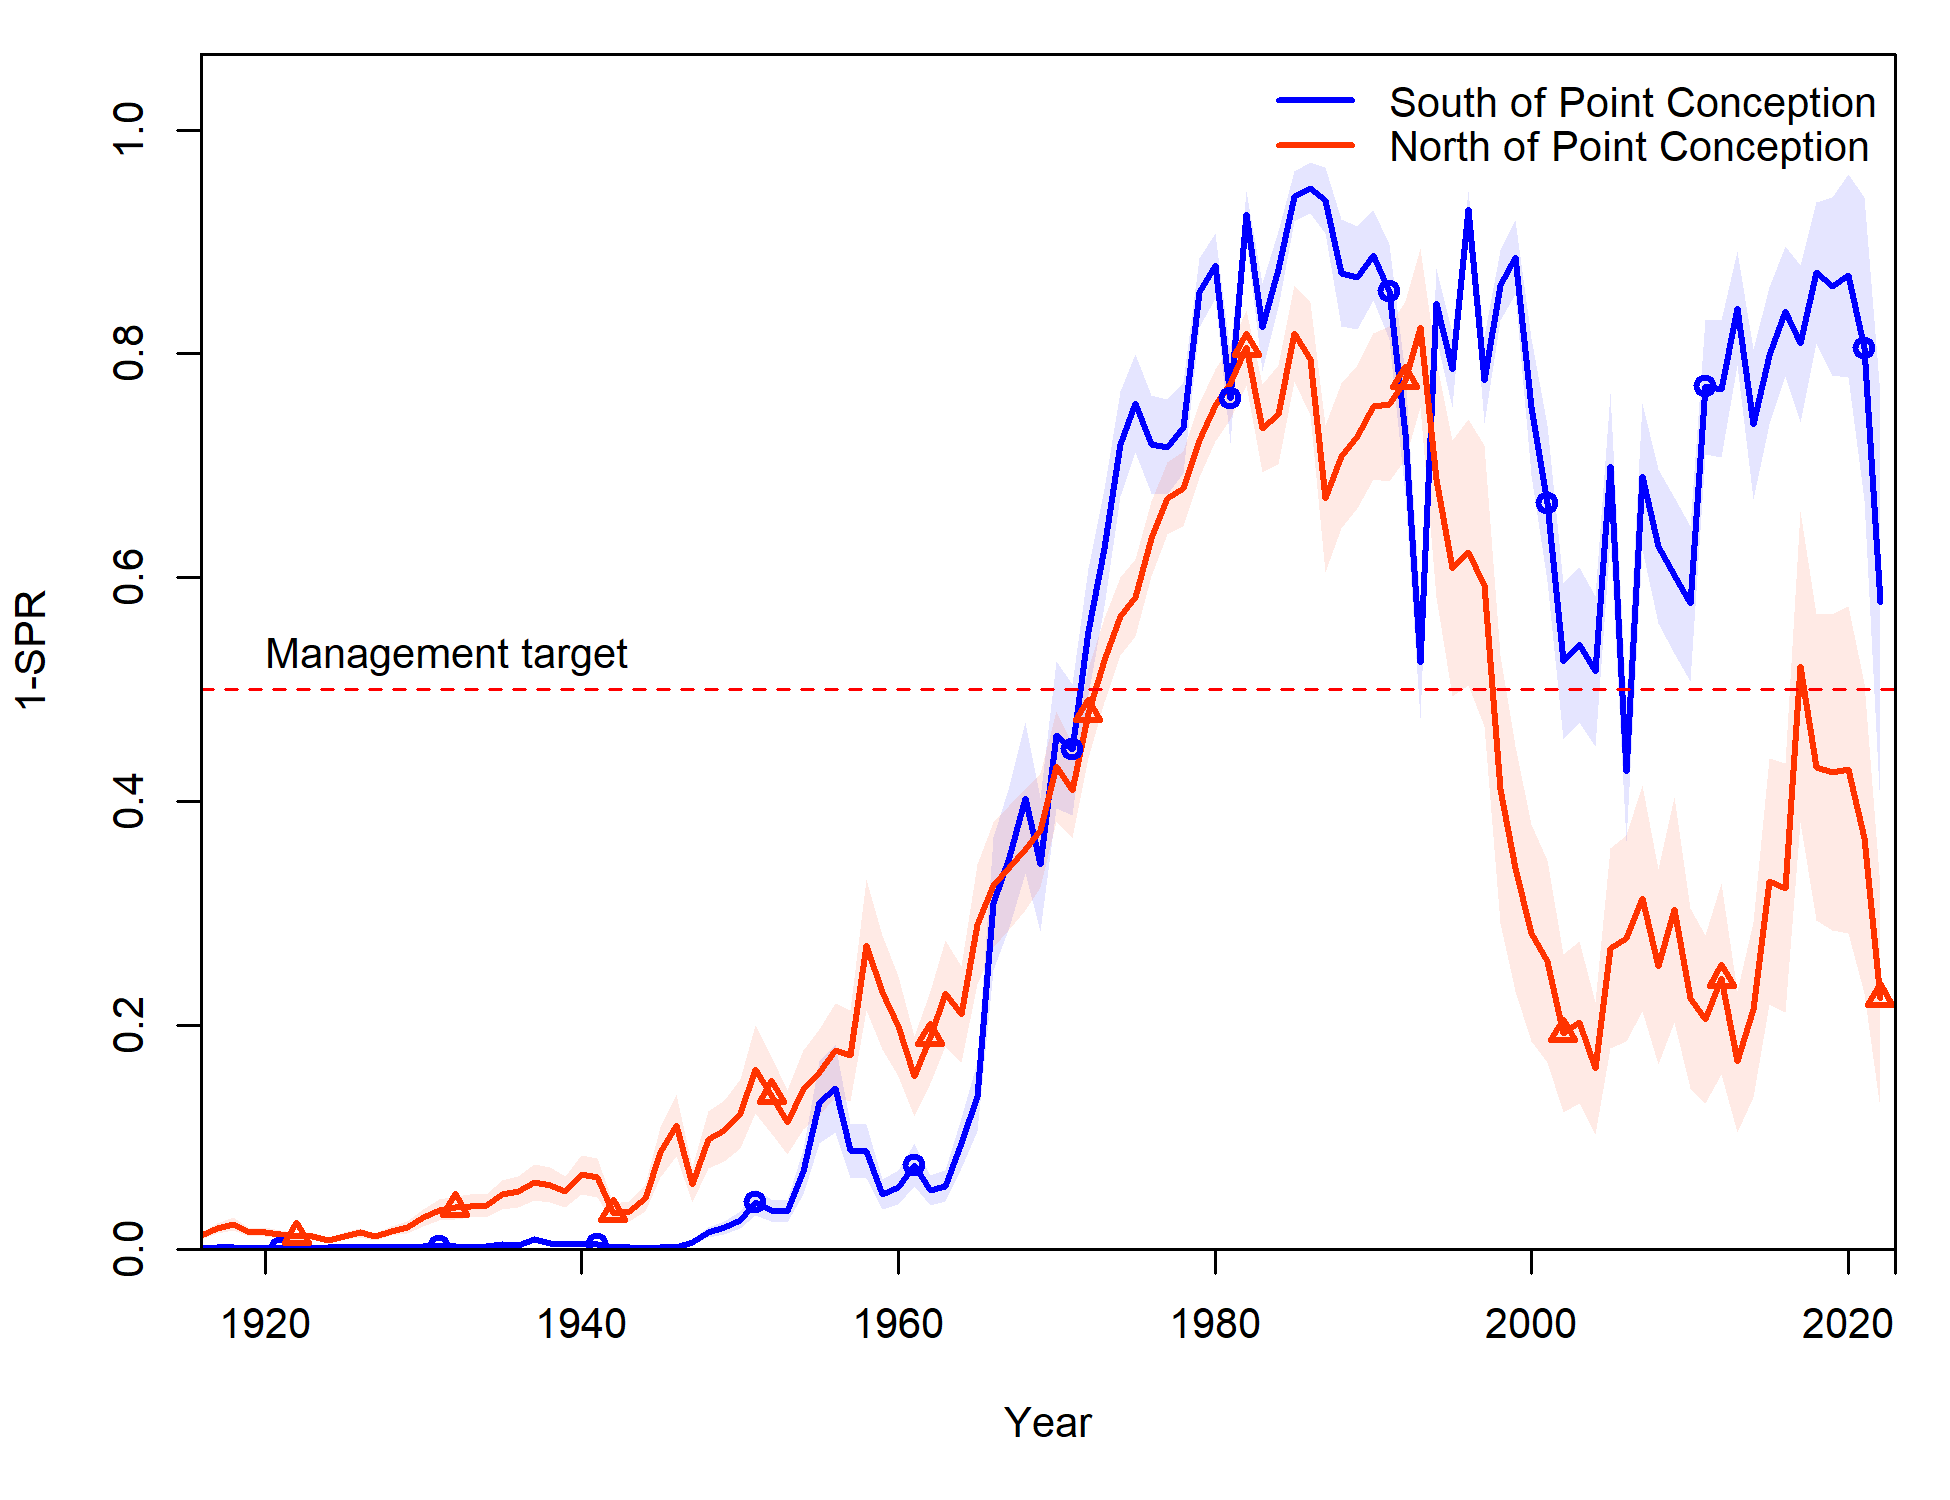
\includegraphics[width=1\textwidth,height=1\textheight]{C:/Users/melissa.monk/Documents/GitHub/copper_rockfish_2023/documents/shared_figures/compare6_SPRratio_uncertainty.png}
\caption{Estimated 1 - relative spawning ratio (SPR) by year for the model areas south and north of Point Conception. The management target is plotted as a red horizontal line and values above this reflect harvest in excess of the proxy harvest rate.\label{fig:es-1-spr}}
\end{figure}

\hypertarget{ecosystem-considerations}{%
\subsection*{Ecosystem considerations}\label{ecosystem-considerations}}
\addcontentsline{toc}{subsection}{Ecosystem considerations}

shared text

\hypertarget{reference-points}\), i.e., the \(B_{MSY}\) proxy and the equilibrium stock size that results from fishing at the default harvest rate, i.e., the \(F_{MSY}\) proxy. Include Table of estimated reference points for ssb, SPR, exploitation rate, and yield based on SSB proxy for MSY, SPR proxy for MSY, and estimated MSY values.

\begingroup\fontsize{10}{12}\selectfont
\begingroup\fontsize{10}{12}\selectfont

\begin{longtable}[t]{r>{\centering\arraybackslash}p{2cm}>{\centering\arraybackslash}p{2cm}>{\centering\arraybackslash}p{2cm}}
\caption{\label{tab:south-referenceES}Summary of reference points and management quantities, including estimates of the 95 percent intervals for the sub-area model south of Point Conception.}\\
\toprule
 & Estimate & Lower Interval & Upper Interval\\
\midrule
\endfirsthead
\caption[]{Summary of reference points and management quantities, including estimates of the 95 percent intervals for the sub-area model south of Point Conception. \textit{(continued)}}\\
\toprule
 & Estimate & Lower Interval & Upper Interval\\
\midrule
\endhead

\endfoot
\bottomrule
\endlastfoot
Unfished Spawning Output & 201.06 & 163.43 & 238.70\\
Unfished Age 3+ Biomass (mt) & 1999.51 & 1624.90 & 2374.12\\
Unfished Recruitment (R0) & 241.18 & 196.04 & 286.32\\
Spawning Output (2023) & 32.06 & 12.70 & 51.42\\
Fraction Unfished (2023) & 0.16 & 0.06 & 0.25\\
Reference Points Based SB40\% &  &  & \\
Proxy Spawning Output SB40\% & 80.43 & 65.37 & 95.48\\
SPR Resulting in SB40\% & 0.46 & 0.46 & 0.46\\
Exploitation Rate Resulting in SB40\% & 0.06 & 0.05 & 0.06\\
Yield with SPR Based On SB40\% (mt) & 49.99 & 40.74 & 59.25\\
Reference Points Based on SPR Proxy for MSY &  &  & \\
Proxy Spawning Output (SPR50) & 89.71 & 72.92 & 106.50\\
SPR50 & 0.50 & - & -\\
Exploitation Rate Corresponding to SPR50 & 0.05 & 0.05 & 0.05\\
Yield with SPR50 at SB SPR (mt) & 47.78 & 38.93 & 56.62\\
Reference Points Based on Estimated MSY Values &  &  & \\
Spawning Output at MSY (SB MSY) & 55.51 & 45.15 & 65.87\\
SPR MSY & 0.35 & 0.34 & 0.35\\
Exploitation Rate Corresponding to SPR MSY & 0.08 & 0.08 & 0.08\\
MSY (mt) & 52.94 & 43.14 & 62.74\\*
\end{longtable}
\endgroup{}
\endgroup{}


\begingroup\fontsize{10}{12}\selectfont
\begingroup\fontsize{10}{12}\selectfont

\begin{longtable}[t]{r>{\centering\arraybackslash}p{2cm}>{\centering\arraybackslash}p{2cm}>{\centering\arraybackslash}p{2cm}}
\caption{\label{tab:north-referenceES}Summary of reference points and management quantities, including estimates of the 95 percent intervals for the sub-area model north of Point Conception.}\\
\toprule
 & Estimate & Lower Interval & Upper Interval\\
\midrule
\endfirsthead
\caption[]{Summary of reference points and management quantities, including estimates of the 95 percent intervals for the sub-area model north of Point Conception. \textit{(continued)}}\\
\toprule
 & Estimate & Lower Interval & Upper Interval\\
\midrule
\endhead

\endfoot
\bottomrule
\endlastfoot
Unfished Spawning Output & 486.15 & 387.43 & 584.87\\
Unfished Age 3+ Biomass (mt) & 4719.91 & 3777.92 & 5661.90\\
Unfished Recruitment (R0) & 567.77 & 452.48 & 683.06\\
Spawning Output (2023) & 262.10 & 124.28 & 399.92\\
Fraction Unfished (2023) & 0.54 & 0.32 & 0.76\\
Reference Points Based SB40\% &  &  & \\
Proxy Spawning Output SB40\% & 194.46 & 154.97 & 233.95\\
SPR Resulting in SB40\% & 0.46 & 0.46 & 0.46\\
Exploitation Rate Resulting in SB40\% & 0.06 & 0.06 & 0.06\\
Yield with SPR Based On SB40\% (mt) & 129.86 & 104.05 & 155.67\\
Reference Points Based on SPR Proxy for MSY &  &  & \\
Proxy Spawning Output (SPR50) & 216.90 & 172.85 & 260.94\\
SPR50 & 0.50 &  & \\
Exploitation Rate Corresponding to SPR50 & 0.05 & 0.05 & 0.05\\
Yield with SPR50 at SB SPR (mt) & 124.05 & 99.39 & 148.71\\
Reference Points Based on Estimated MSY Values &  &  & \\
Spawning Output at MSY (SB MSY) & 134.17 & 106.84 & 161.51\\
SPR MSY & 0.35 & 0.34 & 0.35\\
Exploitation Rate Corresponding to SPR MSY & 0.09 & 0.08 & 0.09\\
MSY (mt) & 137.59 & 110.25 & 164.92\\*
\end{longtable}
\endgroup{}
\endgroup{}


\begin{figure}
\centering
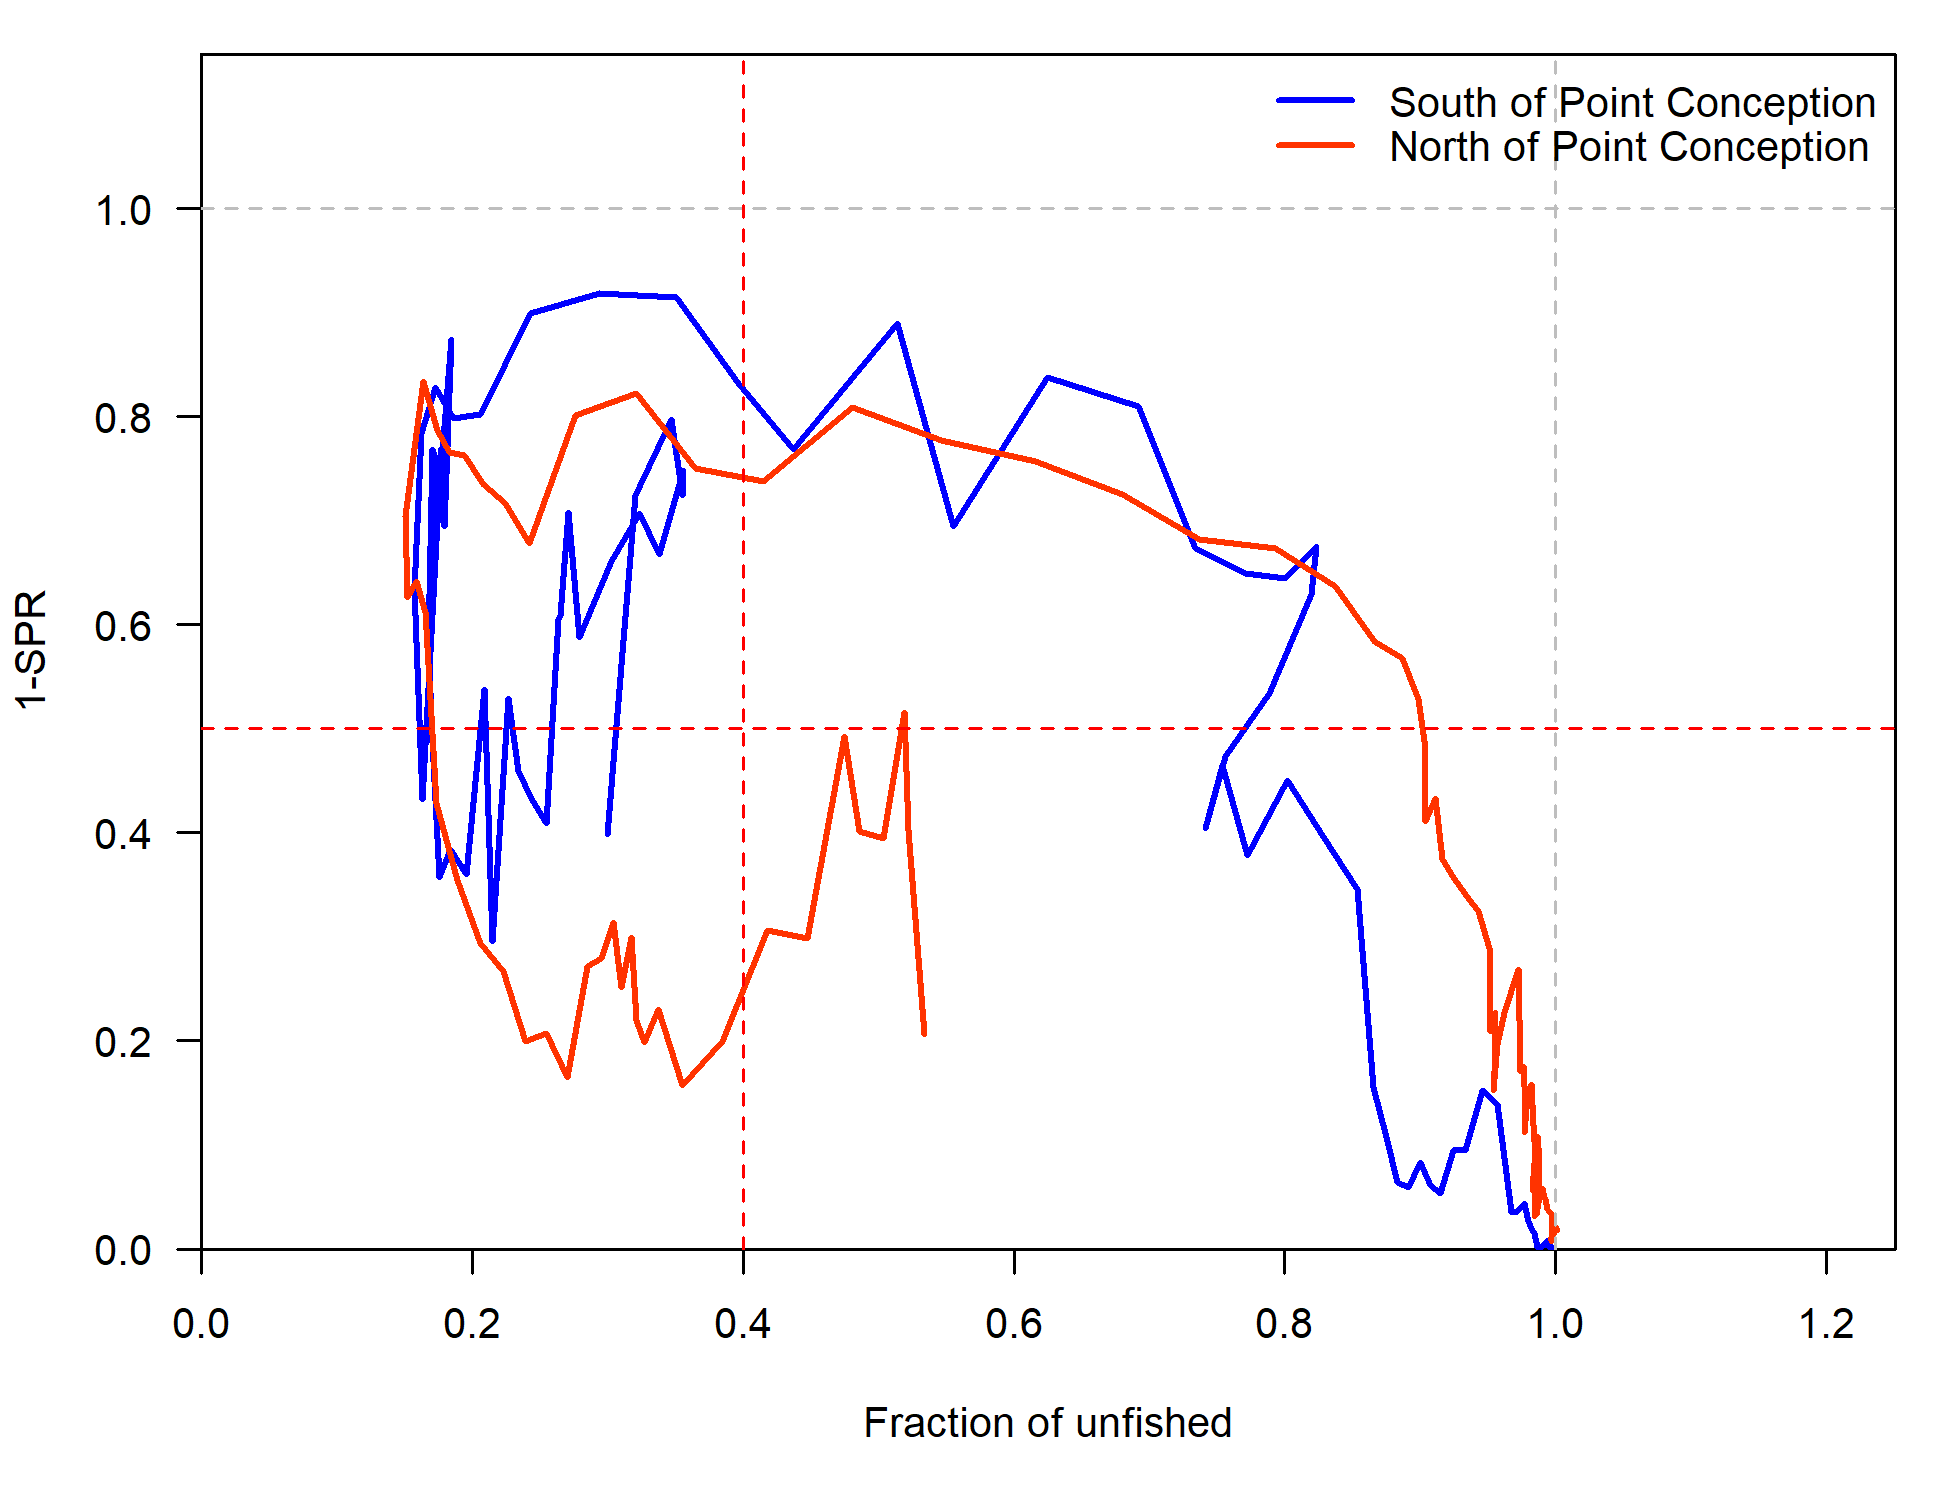
\includegraphics[width=1\textwidth,height=1\textheight]{C:/Users/melissa.monk/Documents/GitHub/copper_rockfish_2023/documents/shared_figures/compare15_phase_plot.png}
\caption{Phase plot of estimated 1-SPR versus fraction unfished for the model areas south and north of Point Conception.\label{fig:es-phase}}
\end{figure}

\begin{figure}
\centering
\includegraphics[width=1\textwidth,height=1\textheight]{S:/copper_rockfish_2023/models/sca/5.5_est_m/plots/yield2_yield_curve_with_refpoints.png}
\caption{Equilibrium yield curve for the base case model for model south of Point Conception. Values are based on the 2022 fishery selectivities and with steepness fixed at 0.72.\label{fig:south-es-yield}}
\end{figure}

\begin{figure}
\centering
\includegraphics[width=1\textwidth,height=1\textheight]{S:/copper_rockfish_2023/models/nca/8.5_update_deb_index/plots/yield2_yield_curve_with_refpoints.png}
\caption{Equilibrium yield curve for the base case model for model north of Point Conception. Values are based on the 2022 fishery selectivities and with steepness fixed at 0.72.\label{fig:north-es-yield}}
\end{figure}

\hypertarget{management-performance}{%
\subsection*{Management performance}\label{management-performance}}
\addcontentsline{toc}{subsection}{Management performance}

Include Table of most recent 10 years of catches in comparison with OFL, ABC, HG, and OY/ACL values, overfishing levels, actual catch and discard. Include OFL (encountered), OFL (retained), and OFL (dead) if different due to discard and discard mortality.

\begingroup\fontsize{10}{12}\selectfont
\begingroup\fontsize{10}{12}\selectfont

\begin{longtable}[t]{c>{\centering\arraybackslash}p{2cm}>{\centering\arraybackslash}p{2cm}>{\centering\arraybackslash}p{2cm}}
\caption{\label{tab:es-ca-management}The portion of the Overfishing Limit (OFL) and Annual Catch Limit (ACL) and estimated catch in California waters.}\\
\toprule
Year & OFL (mt) & ACL (mt) & Catch (mt)\\
\midrule
\endfirsthead
\caption[]{\label{tab:es-ca-management}The portion of the Overfishing Limit (OFL) and Annual Catch Limit (ACL) and estimated catch in California waters. \textit{(continued)}}\\
\toprule
Year & OFL (mt) & ACL (mt) & Catch (mt)\\
\midrule
\endhead

\endfoot
\bottomrule
\endlastfoot
2012 & 163.15 & 136.17 & 85.95\\
2013 & 148.00 & 123.42 & 105.18\\
2014 & 148.00 & 123.42 & 98.65\\
2015 & 303.75 & 277.32 & 147.64\\
2016 & 286.88 & 261.95 & 165.27\\
2017 & 313.70 & 286.38 & 225.48\\
2018 & 319.60 & 291.85 & 203.69\\
2019 & 325.08 & 296.83 & 182.59\\
2020 & 330.35 & 301.60 & 242.73\\
2021 & 249.85 & 206.43 & 164.20\\
2022 & 249.48 & 204.02 & 66.67\\*
\end{longtable}
\endgroup{}
\endgroup{}

\hypertarget{unresolved-problems-and-major-uncertainties}{%
\subsection*{Unresolved problems and major uncertainties}\label{unresolved-problems-and-major-uncertainties}}
\addcontentsline{toc}{subsection}{Unresolved problems and major uncertainties}

shared text

\hypertarget{decision-table-and-projections}{%
\subsection*{Decision table and projections}\label{decision-table-and-projections}}
\addcontentsline{toc}{subsection}{Decision table and projections}

Replace text with projected yields (OFL, ABC, and ACL), spawning biomass, and stock depletion levels for each year. OFL calculations should be based on the assumption that future catches equal ABCs and not OFLs.

\begingroup\fontsize{10}{12}\selectfont

\begin{landscape}\begingroup\fontsize{10}{12}\selectfont

\begin{longtable}[t]{c>{\centering\arraybackslash}p{1.38cm}>{\centering\arraybackslash}p{1.38cm}>{\centering\arraybackslash}p{1.38cm}>{\centering\arraybackslash}p{1.38cm}>{\centering\arraybackslash}p{1.38cm}>{\centering\arraybackslash}p{1.38cm}>{\centering\arraybackslash}p{1.38cm}}
\caption{\label{tab:es-ca-proj}The estimated spawning output in number of million eggs across California and fraction unfished by year.}\\
\toprule
Year & Adopted OFL (mt) & Adopted ABC (mt) & Assumed Catch (mt) & OFL (mt) & ABC (mt) & Spawning Biomass & Fraction Unfished\\
\midrule
\endfirsthead
\caption[]{\label{tab:es-ca-proj}The estimated spawning output in number of million eggs across California and fraction unfished by year. \textit{(continued)}}\\
\toprule
Year & Adopted OFL (mt) & Adopted ABC (mt) & Assumed Catch (mt) & OFL (mt) & ABC (mt) & Spawning Biomass & Fraction Unfished\\
\midrule
\endhead

\endfoot
\bottomrule
\endlastfoot
2023 & 116.4 & 91.53 & 91.5 & - & - & 331.05 & 0.481\\
2024 & 121.32 & 94.69 & 94.7 & - & - & 331.91 & 0.482\\
2025 & - & - & - & 182.58 & 169.79 & 331.76 & 0.482\\
2026 & - & - & - & 182.54 & 169.45 & 330.85 & 0.481\\
2027 & - & - & - & 182.16 & 169.11 & 329.74 & 0.479\\
2028 & - & - & - & 181.54 & 168.81 & 328.80 & 0.478\\
2029 & - & - & - & 180.82 & 168.58 & 328.09 & 0.477\\
2030 & - & - & - & 180.13 & 168.42 & 327.58 & 0.476\\
2031 & - & - & - & 179.53 & 168.35 & 327.20 & 0.475\\
2032 & - & - & - & 179.02 & 168.33 & 326.90 & 0.475\\
2033 & - & - & - & 178.61 & 168.37 & 326.66 & 0.474\\
2034 & - & - & - & 178.28 & 168.44 & 326.45 & 0.474\\*
\end{longtable}
\endgroup{}
\end{landscape}
\endgroup{}

\hypertarget{scientific-uncertainty}{%
\subsection*{Scientific uncertainty}\label{scientific-uncertainty}}
\addcontentsline{toc}{subsection}{Scientific uncertainty}

The model estimated uncertainty around the 2023 spawning output was \(\sigma\) = 0.22 and the uncertainty around the OFL was \(\sigma\) = 0.22. This is likely an underestimate of overall uncertainty because of the necessity to fix several population dynamic parameters (e.g., steepness, recruitment variance, female natural mortality) and no explicit incorporation of model structural uncertainty (although see the decision table for alternative states of nature).

\hypertarget{research-and-data-needs}{%
\subsection*{Research and data needs}\label{research-and-data-needs}}
\addcontentsline{toc}{subsection}{Research and data needs}

shared text

\pagebreak
\setlength{\parskip}{5mm plus1mm minus1mm}
\pagenumbering{arabic}
\setcounter{page}{1}
\renewcommand{\thefigure}{\arabic{figure}}
\renewcommand{\thetable}{\arabic{table}}
\setcounter{table}{0}
\setcounter{figure}{0}

\hypertarget{introduction}{%
\section{Introduction}\label{introduction}}

\hypertarget{basic-information-and-life-history}{%
\subsection{Basic Information and Life History}\label{basic-information-and-life-history}}

This assessment report describes the sub-area population of copper rockfish (\emph{Sebastes caurinus}) off the California coast south of Point Conception in U.S. waters, using data through 2022. The sub-area population north of Point Conception in California waters was also evaluated and is described in a separate assessment report. The copper rockfish status for the California stock of is determined by the combined estimates of spawning output from both sub-areas and is detailed in the \protect\hyperlink{management}{management} section. This assessment does not account for populations located in Mexico waters or other areas off the U.S. coast and assumes that these southern and northern populations do not contribute to the population being assessed here.

Copper rockfish have historically been a part of both commercial and recreational fisheries throughout its range. Copper rockfish are a demersal, relatively nearshore species within the subgenus \emph{Pteropodus.} Copper rockfish range from xxx to xx at depth of xxx (M. S. Love, Yoklavich, and Thorsteinson 2002). The core range is comparatively large, from northern Baja Mexico to the Gulf of Alaska, with copper rockfish also found in Puget Sound. Copper rockfish are commonly found in waters less than 100 meters in depth inhabiting nearshore kelp forests and complex low-relief rocky habitat (M. Love 1996). Adult copper rockfish have high site fidelity and do not make long-range movements. An acoustic telemetry study displaced copper rockfish 4km from their capture location to an artificial reef and within 10 days, half of the copper rockfish returned to the original capture location (Reynolds, Powers, and Bishop 2010).

long the posterior two-thirds of the lateral line. The copper rockfish has high variation in coloration throughout its range, taking on coloration from dark brown, olive, orange-red and pink, with patches of yellow and pink (D. J. Miller and Lea 1972). In general the copper rockfish towards the northern part of the range are often darker in color than fish encountered in southern California. The distinct change in coloration resulted in copper rockfish described as two separate species, copper rockfish (\emph{S. caurinus}) and whitebelly rockfish (\emph{S. vexillaris}).

The \emph{Sebastes} genus are viviparous with internal fertilization, many exhibit dimorphic growth with females larger at size-at-age than males, and a number of species have reproductive strategies that vary with latitude. There are very few fecundity samples from copper rockfish available from available from California, although copper rockfish are assumed to produce a single brood annually. In southern California, peak parturition occurs xxxx central California peak parturition occurs in February and March.

The pelagic larvae are encountered in the CalCOFI surveys, but neither larval nor young-of-the-year (YOY) can be identified copper rockfish visually (Thompson et al. 2017). The size at birth ranges from 5-6 mm and the larvae remain pelagic until approximately 22-23 mm standard length at which time they recruit to the kelp forest canopy (T. W. Anderson 1983).

Juvenile Copper rockfish are indistinguishable from kelp (\emph{S. atrovirens}), black-and-yellow (\emph{S. chrysomelas}), and gopher rockfish (\emph{S. carnatus}), all of which recruit to the kelp forest canopy in the spring months. Copper rockfish is the first of the species group to recruit to the kelp forest from April to May and can be distinguished from the other species once it reaches a size around 50 mm standard length (T. W. Anderson 1983). Baetscher genetically identified YOY rockfish from surveys in Carmel and Monterey Bays in California and provided the authors with the length and genotyped species idenifications from her study (Baetscher et al. 2019). The average length of copper rockfish in July was 3-4 cm total length \ref{fig:copper-smurf-length}. Anderson observed benthic copper rockfish nocturnally active over sandy bottom outside the kelp forest (T. W. Anderson 1983).

Copper rockfish are a relatively long-lived rockfish, estimated to live at least 50 years (M. Love 1996). Copper rockfish was determined to have the highest vulnerability (V = 2.27) of any West Coast groundfish stock evaluated in a productivity susceptibility analysis (Cope et al. 2011). This analysis calculated species-specific vulnerability scores based on two dimensions: productivity characterized by the life history and susceptibility that characterized how the stock could be impacted by fisheries and other activities.

As adults, there is little evidence of movement, with Hanan and CCFRP citations

Copper rockfish are opportunistic carnivores and commonly consume crustaceans, mollusks, and fish whole (Lea, McAllister, and VenTresca 1999; Bizzarro, Yoklavich, and Wakefield 2017). -Prince (1972) observed a shift in a diet dominated by arthropods in age 0 and 1 fish, and a shift to a more diverse diet including molluscs and fish as they aged. the study also noted that juvenile copper rockfish were predated on by harbor seals and lingcod.

There is currently no evidence of significant stock structure from genetic studies of copper rockfish across the west coast. -Buonaccorsi et al. (2002) looked at genetic variation across six micosatellite DNA loci from samples ranging from British Columbia to southern California. Significant population subdivision was detected between th Puget Sound and coastal samples and support the model of isolation-by-distance for copper rockfish. Sivasundar and Palumbi (2010) conducted a genetic study to determine the potential for biogeographic boundaries to prohibit gene flow for 15 \emph{Sebastes} species. The study's sample sizes of copper rockfish with samples form Oregon, Monterey Bay and Santa Barbara. Sivasundar and Palumbi (2010) used mtDNA and could differentiate samples from Santa Barbara from those collected in Oregon and Monterey Bay, but the Monterey Bay and Oregon samples could not be distinguished. Micosatellite data did not reveal any genetic differentiation among the sampels from the three locations for copper rockfish and suggests low genetic differentiation coastwide.

The most recent genetic analysis of copper rockfish to date was conducted by Johansson et al. (2008). The study included 749 samples from along the west coast ranging from Neah Bay, Washington to San Diego, California with the majority of sampling locations clustered north of Cape Mendocino in northern California. The study included 185 samples collected within California. Eleven microsatellite DNA loci were analyzed. The study found significant evidence to support isolation by distance at the coast wide scale. Weak, but significant, genetic structure was identified from samples collected along the Oregon coast suggesting that habitat barriers may limit larval dispersal.

\hypertarget{ecosystem-considerations-1}{%
\subsection{Ecosystem Considerations}\label{ecosystem-considerations-1}}

This stock assessment does not explicitly incorporate trophic interactions, habitat factors (other than as they inform relative abundance indices) or environmental factors into the assessment model, but a brief description of likely or potential ecosystem considerations are provided below.

As with most other rockfish and groundfish in the California Current, recruitment, or cohort (year-class) strength appears to be highly variable for the copper rockfish complex, with only a modest apparent relationship to estimated levels of spawning output. Oceanographic and ecosystem factors are widely recognized to be key drivers of recruitment variability for most species of groundfish, as well as most elements of California Current food webs. Empirical estimates of recruitment from pelagic juvenile rockfish surveys have been used to inform incoming year class strength for some of these stocks, however copper rockfish are infrequently encountered in these surveys. Between 1998 and 2013 the California Cooperative Oceanic Fisheries Investigation (CalCOFI) survey observed had 34 positive observations copper rockfish out of nearly 300,000 total juvenile \emph{Sebastes} encountered in juvenile surveys.

\hypertarget{historical-and-current-fishery-information}{%
\subsection{Historical and Current Fishery Information}\label{historical-and-current-fishery-information}}

Off the coast of California south of Point Conception copper rockfish is caught in both commercial and recreational fisheries. Recreational removals have been the largest source of fishing mortality of copper rockfish across all years (Table \ref{tab:allcatches} and Figure \ref{fig:catch}). The recreational fishery is comprised of individual recreational fishers (Private/Rental, PR) and charter recreational private vessels (CPFV) which take groups of individuals out for day fishing trips. Across both types of recreational fishing the majority of effort occurs around rocky reefs that can be accessed via a day-trips.

The recreational fishery in the early part of the 20th century was focused on nearshore waters near ports, with expanded activity further from port and into deeper depths over time (R. R. Miller et al. 2014). Prior to the groundfish fishery being declared a federal disaster in 2000, and the subsequent rebuilding period, there were no time or area closures for groundfish. Access to deeper depths during this period spread effort over a larger area and filled bag limits with a greater diversity of species from both the shelf and nearshore. This resulted in lower catch of nearshore rockfish relative to the period after 2000 when 20 to 60 fm depth restrictions ranging from 20 fm in the Northern Management Area to 60 fm in the Southern Management Area were put in place in various management area delineations along the state. This shifting effort onto the nearshore, concomitantly increased catch rates for nearshore rockfish including copper rockfish in the remaining open depths, though season lengths were greatly curtailed.

Following all previously overfished groundfish species, other than yelloweye rockfish, being declared rebuilt by 2019, deeper depth restrictions were offered in the Southern Management area allowing resumed access to shelf rockfish in less than 75 fm and are currently 100 fm as of 2021. The increased access to deeper depths south of Point Conception with the rebuilding of cowcod is expected to reduce the effort in nearshore waters where copper rockfish is most prevalent. To the north of Point Conception where yelloweye rockfish are prevalent, depth constraints persist and effort remains focused on the nearshore in 30 to 50 fm depending on the management area. As yelloweye rockfish continues to rebuild, incremental increases in access to deeper depths are expected, which will likely further reduce the effort in nearshore waters where copper rockfish is most prevalent.

Prior to development of the live fish market in the 1980s, there was very little commercial catch of copper rockfish, with dead copper rockfish fetching a low ex-vessel price per pound. Copper rockfish were targeted along with other rockfish to some degree in the nearshore or caught as incidental catch by vessels targeting other more valuable stocks such as lingcod. Most fish were caught using hook and line gear, though some were caught using traps, gill nets and, rarely, trawl gear. Trawling was prohibited within three miles of shore in 1953 and gill netting within three miles of shore was prohibited in 1994, preventing access to a high proportion of the species habitat with these gear types. Copper rockfish were caught along with other rockfish to some degree in the nearshore or caught as bycatch by vessels targeting other more valuable stocks such as lingcod.

In the late 1980s and early 1990s a market for fish landed live arose out of Los Angeles and the Bay area, driven by demand from Asian restaurants and markets. The growth of the live fish market was driven by consumers willing to pay a higher price for live fish, ideally plate-sized (12 - 14 inches or 30.5 - 35.6 cm). Live fish landed for the restaurant market are lumped into two categories, small (1 - 3 lbs.) or large (3 - 6 lbs.), with small, plate-sized, fish fetching higher prices at market ranging between \$5 -7 per fish (Bill James, personal communication). Copper rockfish is one of the many rockfish species that is included in the commercial live fish fishery. The proportion of copper rockfish being landed live vs.~dead since 2000 by California commercial fleets ranges between 50 to greater than 70 percent in the southern and northern areas, respectively.

With the development and expansion of the nearshore live fish fishery during the 1980s and 1990s, new entrants in this open access fishery were drawn by premium ex-vessel price per pound for live fish, resulting in over-capitalization of the fishery. Since 2002, the California Department of Fish and Wildlife (CDFW) has managed 19 nearshore species in accordance with Nearshore Fisheries Management Plan (Wilson-Vandenberg, Larinto, and Key 2014). In 2003, the CDFW implemented a Nearshore Restricted Access Permit system, including the requirement of a Deeper Nearshore Fishery Species Permit to retain copper rockfish, with the overall goal of reducing the number of participants to a more sustainable level, with permit issuance based on historical landings history by the retrospective qualifying date. The result was a reduction in permits issued from 1,127 in 1999 to 505 in 2003, greatly reducing catch levels. In addition, reduced trip limits, season closures in March and April and depth restrictions were implemented to address bycatch of overfished species and associated constraints from their low catch limits.

Copper rockfish residing between Point Conception and the California/Oregon border are assessed here as a single, separate stock (Figure \ref{fig:ca-map}). This designation was made based on oceanographic, geographic, and fishery conditions. The copper rockfish population in California waters was split at Point Conception due to water circulation patterns that create a natural barrier between nearshore rockfish populations to the north and south. The northern border for this assessment was defined as the California/Oregon border due to substantial differences in historical and current exploitation levels. Additionally, the fairly sedentary nature of adult copper rockfish, likely limits flow of fish between northern California and areas to the north.

\hypertarget{summary-of-management-history-and-performance}{%
\subsection{Summary of Management History and Performance}\label{summary-of-management-history-and-performance}}

Replace text.

\hypertarget{foreign-fisheries}{%
\subsection{Foreign Fisheries}\label{foreign-fisheries}}

Replace text.

\hypertarget{data}{%
\section{Data}\label{data}}

Data comprise the foundational components of stock assessment models. The decision to include or exclude particular data sources in an assessment model depends on many factors. These factors often include, but are not limited to, the way in which data were collected (e.g., measurement method and consistency); the spatial and temporal coverage of the data; the quantity of data available per desired sampling unit; the representativeness of the data to inform the modeled processes of importance; timing of when the data were provided; limitations imposed by the Terms of Reference; and the presence of an avenue for the inclusion of the data in the assessment model. Attributes associated with a data source can change through time, as can the applicability of the data source when different modeling approaches are explored (e.g., stock structure or time-varying processes). Therefore, the specific data sources included or excluded from this assessment should not necessarily constrain the selection of data sources applicable to future stock assessments for copper rockfish. Even if a data source is not directly used in the stock assessment they can provide valuable insights into biology, fishery behavior, or localized dynamics.

Data from a wide range of programs were available for possible inclusion in the current assessment model. Descriptions of each data source included in the model (Figure \ref{fig:data-plot}) and sources that were explored but not included in the base model are provided below. Data that were excluded from the base model were explicitly explored during the development of this stock assessment or have not changed since their past exploration in a previous copper rockfish stock assessment. In some cases, the inclusion of excluded data sources were explored through sensitivity analyses (see Section \ref{assessment-model}).

\hypertarget{fishery-dependent-data}{%
\subsection{Fishery-Dependent Data}\label{fishery-dependent-data}}

\hypertarget{commercial-fishery}{%
\subsubsection{Commercial Fishery}\label{commercial-fishery}}

\hypertarget{landings-and-discards}{%
\paragraph{Landings and Discards}\label{landings-and-discards}}

\hfill\break

Commercial landings prior to 1969 were extracted from the Southwest Fisheries Science Center (SWFSC) landings reconstruction database for estimates from the California Catch Reconstruction (Ralston et al. 2010). Landings in this database are divided into trawl, non-trawl, and unknown gear categories. Regions 7 and 8 as defined by Ralston et al. (2010) were assigned to south of Point Conception in California. Regions 2, 4, and 5 are associated with areas north of Point Conception. Region 6 in Ralston et al. (2010) included Santa Barbara County (mainly south of Point Conception), plus some major ports north of Point Conception. To allocate landings from Region 6 to the areas north and south of Point Conception, we followed an approach used by Dick et al. (2007) for the assessment of cowcod. Specifically, port-specific landings of total rockfish from the CDFW Fish Bulletin series were used to determine the annual fraction of landings in Region 6 that was north and south of Point Conception (Table \ref{tab:com-ratio}). Rockfish landings at that time were not reported at the species level. Although the use of total rockfish landings to partition landings in Region 6 is not ideal, we see this as the best available option in the absence of port-specific species composition data. Landings from unknown locations (Region 0) were allocated proportional to the landings from known regions.

In September 2005, the California Cooperative Groundfish Survey (CCGS) incorporated newly acquired commercial landings statistics from 1969-1980 into the CALCOM database (Pearson, Erwin, and Key 2008). The data consisted of landing receipts (``fish tickets''), including mixed species categories for rockfish. In order to assign rockfish landings to individual species, the earliest available species composition samples were applied to the fish ticket data by port, gear, and quarter. These `ratio estimator' landings are coded (internally) as market category 977 in the CALCOM database, and are used in this and past assessments as the best available landings for the time period 1969-1980 for all port complexes. See Appendix A of Dick et al. (2007) for further details. Commercial fishery landings from 1981-2022 were extracted from the Pacific Fisheries Information Network (PacFIN) database (extracted February 6, 2023). Landings were separated north and south of Point Conception based on port of landing. Commercial landings for copper rockfish were split into two fleets based on the fish landed condition, live or dead, and aggregated across gear types (Table \ref{tab:allcatches} and Figure \ref{fig:catch}). The selection of this fleet structure was based on potential differences in selectivity by the fishery based on fish landed condition where the live fish fishery may be targeting fish of particular sizes (i.e., plate sized). The first year where fish were observed to be landed live for copper rockfish in the area south of Point Conception was 1994.

Discarding was not estimated within the model. The commercial catches, landings plus discards, were estimated external to the model based on data from the West Coast Groundfish Observer Program (WCGOP) data provided in the Groundfish Expanded Mortality Multiyear (GEMM) product. The GEMM provides expanded estimates of landings, discard, and catches based on observed trips by sector split north and south of 40\(^\circ\) 10' N. lat. for the commercial fishery. Estimated landings and discards south of 40\(^\circ\) 10' N. lat. from select sectors (LE Fixed Gear DTL - Hook and Line, Nearshore, CS - Hook and Line, OA Fixed Gear - Hook and Line, OA Fixed Gear - Pot, and LE Fixed Gear DTL - Pot) were used to calculate a discard rate (total discard divided by the sum of landings and discards by year) for 2002-2021. The annual discard rates were applied to the total landings by year to calculate catches for both areas south and north of Point Conception. The median discard rate south of 40\(^\circ\) 10' N. lat. from the select sectors between 2002-2021 in the GEMM was 3 percent. This discard rate was applied to landings between 1916-2001 and 2022 to determine catch by year. The assumptions around the discard rate by year had limited impact to the assumed total catches given the limited scale of removals by the commercial fishery for copper rockfish. Across all years, 1916-2022, the landings were increased by 2-3 percent by area (11 mt south of Point Conception and 26 mt north of Point Conception) to calculate the total catches.

\hypertarget{composition-data}{%
\paragraph{Composition Data}\label{composition-data}}

\hfill\break

Biological data were extracted from the PacFIN Biological Data System on March 20, 2023. Length data for the commercial fleet were extracted from the PacFIN Biological Data System (BDS) with samples for north↨ of Point Conception beginning in 1978 (Tables \ref{tab:dead-com-len} and \ref{tab:live-com-len}). The commercial data was split by landed condition, live or dead, with the first data for the live fish fishery beginning in 1994. The number of length samples by fleet were highly variable with the largest number of sample by year being recorded in the 1990s for the dead fish fishery. In recent years, the number of length samples by year are limited for both fleets with the live fish with annual sample sizes less than 100 per year. The number of samples prior to the 1990s and in the 2000s for the dead fish fishery were sparse and variable across sizes. During model explorations any year with less than 20 sampled fish were considered too sparse to accurately reflect the fleet selectivity for that year (see \protect\hyperlink{excluded-data}{Appendix A} for implied fits to these lengths).

The majority of lengths observed by the commercial fleet landed dead copper rockfish ranged between approximately 25 - 50 cm (Figure \ref{fig:com-dead-len-data}, detailed length compositions by year can be found in the Appendix, Section \ref{length-data}). Notably, in the early years of data prior to 1990 observed few smaller fish compared to later years. The mean length observed by year ranged between approximately 30 - 45 cm (Figure \ref{fig:mean-com-dead-len-data}). The mean observed length since 2010 slowly increase through 2018 with a drop in the mean observed age in the most recent years data.

The observed distribution of sizes sampled from the commercial live fish fleet were generally variable prior to 2011 with the length distributions since indicating a smaller range of sizes being landed after 2011 (Figure \ref{fig:com-live-len-data}). The observed mean length of fish landed live also clearly shows a drop in average sizes being landing starting in 2011 (Figure \ref{fig:mean-com-live-len-data}).

The input sample sizes for all commercial data were calculated based on a combination of trips and fish sampled:

\begin{centering}

Input effN = $N_{\text{trips}} + 0.138 * N_{\text{fish}}$ if $N_{\text{fish}}/N_{\text{trips}}$ is $<$ 44

Input effN = $7.06 * N_{\text{trips}}$ if $N_{\text{fish}}/N_{\text{trips}}$ is $\geq$ 44

\end{centering}

\hypertarget{recreational-fishery}{%
\subsubsection{Recreational Fishery}\label{recreational-fishery}}

\hypertarget{landings-and-discards-1}{%
\paragraph{Landings and Discards}\label{landings-and-discards-1}}

\hfill\break

The recreational fishery is the main source of exploitation of copper rockfish across California. The recreational catches of copper rockfish south of Point Conception in California waters peaked in the late 1970s and early 1980s. Catches declined in the 1990s and early 2000s (Table \ref{tab:allcatches} and Figure \ref{fig:catch}). The removals remained relatively low until 2015. Catches begun to increase in 2015, likely due to changes in harvest specifications (\textbf{cope\_data-moderate\_2013?}). The catches decreased in 2020 due to COVID-19 impacts and remained relatively low in 2021 and 2022 due to reductions in the sub-bag limits in California for copper rockfish. The recreational fishery was split into two fleets based on fishing type (termed `modes'), a commercial passenger fishing vessel (CPFV, party/charter mode) fleet and a combined private or rental boats (PR mode) and shoreside (man-made and beach/bank modes) fleet. The catches associated with the shoreside mode for copper rockfish are limited and did not justify a separate fishing fleet within the model.

Recreational landing estimates from 1928 to 1980 were obtained from the historical reconstruction (Ralston et al. 2010). The historical landings reconstruction split removals north and south of Point Conception and by recreational modes. CPFV landings of all rockfish were based on logbook data (which do not report rockfish to the species level), scaled by compliance estimates, while total recreational landings from PR vessels were based on a combination of the relative catch rates observed in the CPFV fleet and a linear ramp between catch estimates in the early 1960s and those in the early 1980s (as described in Ralston et al. (2010)). The species composition of rockfish landings was estimated using a combination of the 1980s Marine Recreational Fisheries Statistics Survey (MRFSS) data as well as limited CPFV mode species composition data from onboard observer programs in the late 1970s (south of Point Conception) and dockside recreational creel surveys in the late 1950s and early 1960s (north of Point Conception).

Recreational removals from 1981-1989 and 1993-2003 were obtained from MRFSS downloaded from the Recreational Fisheries Information Network (RecFIN). Historically, copper rockfish were occasionally referred to as whitebelly rockfish in select California areas. MRFSS catches were pulled for both species names and for all ocean areas. MRFSS includes estimates of removals for 1980. However, due to inconsistencies in the estimates of this year in MRFSS, likely due to it being the first year of the survey with low sample sizes, the value for recreational landings from the historical reconstruction were used (2010).

Some known issues with the MRFSS estimates include 1) a change in the spatial definition of California subregions after 1989, 2) missing or imprecise estimates of catch in weight for some strata that reported catch in numbers, and 3) a hiatus in sampling from 1990-1992 (all modes) and also 1993-1995 in the party/charter mode north of Point Conception. The STAT attempted to address each of these issues, as described below. CRFS estimates from 2004 were also included in the MRFSS analysis, as they were not available on the current RecFIN website but are included with the MRFSS catch estimate tables

The MRFSS definition of ``Southern California'' included San Luis Obispo County between 1981-1989, requiring the catches from this county to be split out and removed from the recreational catch south of Point Conception. The MRFSS catches between southern and northern California were adjusted in a similar fashion as previous assessments split at Point Conception. Albin et al. (1993) used MRFSS data to estimate catch at a finer spatial scale from the California/Oregon border to the southern edge of San Luis Obispo (SLO) County. Over the period 1981-1986, numbers of copper rockfish landed in SLO County were found to be approximately one third (0.317) of the numbers of copper rockfish landed in all California counties north of SLO County (Albin, Karpov, and Van Buskirk 1993). Therefore, to approximate catches north and south of Point Conception from 1980-1989, the STAT reduced the `southern' subregion annual catch (which included SLO County) from 1980-1989 by 0.317 during the same period, and added this amount to the northern subregion catch. On average, this `moves' the estimated SLO County catch from the southern region to the northern region from 1980-1989, creating a spatially consistent time series of landings over the entire time series.

The STAT chose to use catch in terms of weight (WGT\_AB1 column) within MRFSS. The catch weights were converted from kilograms to metric tons and any records with missing catch weights were examined. The number of records with missing catch weights for copper rockfish in MRFSS were limited (only 18 out of 713). The missing catch weights were imputed based on the number of fish (TOT\_CAT column) and the calculated average fish weight by year and area north and south of Point Conception.

MRFSS sampling was halted from 1990-1992 due to funding issues. The survey resumed in 1993 in all modes, except for the PC boat mode which resumed in 1996 for counties north of Santa Barbara County. To produce catch estimates for the missing subregion, mode, and year combinations linear interpolations were used to fill in the missing data.

Two additional revisions were applied to select years and modes in the MRFSS data based on conversations with California Department of Fish and Wildlife (CDFW). The catches for the PR mode north of Point Conception in MRFSS for 1981 were 50 to 90 percent greater than the catches in 1980 and 1982, respectively. The high catches in this year were assumed to be a result of issues in the catch expansions due to limited sampling. The catches for the PR fleet were revised downward to be equal to the average removals in surrounding years (1979, 1980, 1982, and 1983). The catches in MRFSS south of Point Conception in 1987 were identified as abnormally low by CDFW (John Budrick, pers. communication, 13 to 27 percent of catches in 1986 and 1988) which was due to no catch information for waves 1-3 (January - June) for either mode. Absence of data in 1987 for these waves was not observed across other rockfish species in southern California indicating that the absence of catch data was likely not due to closures in the fishery. The catches for this year and mode were set equal to the average catch by mode 2 years before and after 1987.

Recreational landings from 2004-2022 were obtained from California Recreational Fisheries Survey (CRFS) available on RecFIN for for all ocean areas. This survey improves upon the MRFSS sampling design, employing higher sampling rates and producing estimates with finer spatial and temporal resolution. CRFS also employs onboard CPFV observers, providing spatially referenced, drift-level estimates of catch and discard for a subset of anglers on observed groundfish trips. Any CRFS records of fish caught in Mexican waters were removed and catch estimates were split north and south of Point Conception for each fleet. Due to database issues, catches for 2004 are currently not available on RecFIN. The catches for this year were set equal to data pulled in 2021 for the previous assessment of copper rockfish.

Adjustments to the recreational catches for 2020-2022 were provided directly by CDFW to deal with sampling issues due to COVID-19. During 2020 dockside sampling by observers was halted April through June leading to missing catch data within the CRFS database for this period. CDFW provided proxy catch values for these months directly by CRFS district (personal communication, Melanie Parker). The total proxy catches south of Point Conception (districts 1 and 2) for these months were 18.9 mt and 15.0 mt north of Point Conception in California (districts 3 - 6). These catches were split by mode (CPFV and PR) equally for both areas, noting that effort by mode during this period varied across district based on varying COVID-19 restrictions. When sampling resumed a large number of rockfish catches were not identified to species, recorded as rockfish genus, for the remainder of 2020 and 2021 due to social distancing for health and safety. The second adjustment to catches was to allocated unidentified rockfish catches. CDFW provided proxy catch values that allocated a subset of the rockfish genus removals by recreational mode north and south of Point Conception for these years. Finally, the completed catch estimates for 2022 were not available within CRFS on RecFIN by the data deadline for this assessment and estimates were provided directly to the STAT from CDFW.

MRFSS and CRFS both provide estimates of total mortality which combine observed landings plus estimates of discarded fish using depth-dependent mortality rates. While the recreational removals from the historical reconstruction from 1928-1980 account for only landed fish. There is limited information on historical discarding in the recreational fishery. A report by Miller and Gotshall (1965) looked at the number of retained and discard fish in the recreational fishery in California for a select year which showed essentially no discarding of copper rockfish. Based on that no additional discards were applied to the historical data between 1926-190.

\hypertarget{fishery-dependent-indices-of-abundance}{%
\paragraph{Fishery Dependent Indices of Abundance}\label{fishery-dependent-indices-of-abundance}}

\hfill\break

A number of indices of abundance were explored for the recreational fleet. Discarded catch is available from onboard observer surveys, but was not included in indices. Indices developed for the assessment include:

\begin{itemize}
\tightlist
\item
  MRFSS era dockside survey of the CPFV/PC fleet (1980-1999),
\item
  Deb-Wilson Vandenberg survey of the CPFV/PC fleet (1988-1998),
\item
  CDFW CPFV/PC onboard observer index (1999-2019), and
\item
  CRFS PR1 sites dockside survey (2004-2019).
\end{itemize}

Due to limited sampling during 2020 due to the COVID-19 pandemic and inseason action taken by CDFW for 2022 reducing sub-bag limits for copper rockfish across California, both recreational fishery indices of abundance excluded data collected after 2019.

Figure \ref{fig:mrfss-index-main} Appendix Section \ref{mrfss-cpfv-index}

Figure \ref{fig:crfs-index-main} Appendix Section \ref{onboard-cpfv-index}

Figure \ref{fig:dwv-index-main} Appendix Section \ref{dwv-cpfv-index}

Figure \ref{fig:crfs-pr-index-main} Appendix Section \ref{crfs-pr-index}

\hypertarget{composition-data-1}{%
\paragraph{Composition Data}\label{composition-data-1}}

Length compositions were available from the following sources:

\begin{itemize}
\item
  Recreational party/charter mode (CPFV/PC)

  \begin{itemize}
  \tightlist
  \item
    Miller and Goshall dockside survey (1959-1961, 1966)
  \item
    Don Pearson onboard PC survey (1978-1984)
  \item
    MRFSS CPFV/PC dockside survey (1980-1989, 1993-2003)
  \item
    CRFS CPFV/PC onboard dockside survey (2004-2022)
  \item
    Deb Wilson-Vandenberg onboard CPFV survey (1988-1998)
  \end{itemize}
\item
  Recreational private/rental mode (PR)

  \begin{itemize}
  \tightlist
  \item
    Miller and Gotshall dockside PR survey (1959)
  \item
    MRFSS dockside PR survey (1980-1989, 1993-2003)
  \item
    CRFS dockside PR survey (2004-2022)
  \end{itemize}
\end{itemize}

The number of available fish and unique trips by year and fleet are in Tables \ref{tab:rec-len-samps}. MRFSS historical biological data were downloaded from RecFIN website in December 2022. CRFS biological data were also downloaded from RecFIN on February 18, 2023. The Miller and Goshall, Don Person, Deb-Wilson Vandenberg recreational survey data were downloaded from the SWFSC databases in February 2023.

Between 1987 - 1989 and 1993-1998 there were recreational length data for the CPFV fleet from both MRFSS and Deb Wilson-Vandenberg data sets. During data exploration it was determined that the lengths in MRFSS from 1997 and 1998 were also included in the Deb Wilson-Vandenberg indicating that these data sources were duplicative for these years but also potentially other years where they overlapped. In order to avoid double using of data, the length data from MRFSS which had far fewered length samples for the overlapping years with Deb Wilson-Vandenberg for the CPFV fleet were removed from the data used within the model (see \protect\hyperlink{excluded-data}{Appendix A} for implied fits to these lengths).

The majority of length samples for both recreational fleets, CPFV and PR, were unsexed. A wide range of sampled lengths from the recreational CPFV fleet were observed across all years with lengths generally ranging between 25 - 45 cm except for the late 1970s and early 1980s where a higher proportion of larger fish were sampled (Figure \ref{fig:rec-cpfv-len-data}). The mean length of lengths observed in the recreational CPFV fleet since approximately 1990s is relatively stable varying between 35 - 40 cm in length with high variability within the data in the early years (Figure \ref{fig:mean-rec-cpfv-len-data}). The range of lengths sampled from the recreational PR fleet are similar to those from the CPFV fleet with lengths in recent years ranging between 25 - 45 cm with slightly larger proportion of larger fish observed in the 1980s (Figures \ref{fig:rec-pr-len-data} and \ref{fig:mean-rec-pr-len-data}).

Age composition data were available for select years from both the recreational CPFV and PR fleets. Historical age data collected from the CPFV fishery were available from this fleet from 1978, 1981, and 1984. The majority of these fish were sexed (only 4 total unsexed ages from 1978 and 1984) with an average age ranging from 10 to 14 across these years (Figures \ref{fig:rec-cpfv-caal-data} and \ref{fig:mean-rec-cpfv-age-data}). The historical age data from this fleet were input as marginal ages. There were a total of 250 age samples from the final model year, 2022, collected by a cooperative sampling program with the fleet coordinated by the SWFSC (Figures \ref{fig:rec-cpfv-caal-data} and ADD MARGINAL FIGURE). These data were collected by three CPFV vessels that operate north of Point Conception following random sampling protocols. The cooperative ages were compared to all the CPFV lengths collected by the CRFS sampling program to ensure that the sampling was representative of the fishery (Figure \ref{fig:coop-len-comparison} North). These ages were incorporated as either marginal or conditional age-at-length data depending upon how fish length were measured: carcass or whole fish. The carcass lengthed fish were included as marginals in order to avoid any potential measurement bias in the use of these ages. Finally, a total of 139 ages were collected from the PR fleet in 2022 (Figure \ref{fig:rec-pr-caal-data}). These data were used in the model as conditional age-at-length data as well.

The approach to determine the number of unique trips by data source varied. Some data sources had unique trip numbers within the data (Don Pearson, Deb Wilson Vandenberg). Other data sources that lacked clear trip identifier applied a similar methodology as developed by Brian Soper that combines multiple fields of information to attempt to estimate trips sampled. The number of trips for MRFSS data was estimated using the year, wave, ID code, sampling site (INSITE), area, and mode. A similar methodology was done for CRFS and Miller and Gotshall data that used data, county, water area, interview site, and mode.

\hypertarget{fishery-independent-data}{%
\subsection{Fishery-Independent Data}\label{fishery-independent-data}}

\hfill\break

Tow fishery-independent data sources with indices of abundance were included in the base model. These surveys sampled rocky habitat across the area north of Point Conception (Figure \ref{fig:survey-locations}) sampled both areas opens to fishing (termed reference areas) and Marine Protected Areas (MPAs, Figure \ref{fig:ref-mpa}).

\hypertarget{california-cooperative-fisheries-research-program-survey}{%
\subsubsection{California Cooperative Fisheries Research Program Survey}\label{california-cooperative-fisheries-research-program-survey}}

\hypertarget{index-of-abundance}{%
\paragraph{Index of Abundance}\label{index-of-abundance}}

\hfill\break

Since 2007, the \gls{s-ccfrp} has monitored several areas in California to evaluate the performance of \glspl{mpa} and understand nearshore fish populations (R. M. Starr et al. 2015; Wendt and Starr 2009). In 2017, the survey expanded beyond the four \Gls{mpa}s in central California (Año Nuevo, Point Lobos, Point Buchon, and Piedras Blancas) to include the entire California coast. Fish are collected by volunteer anglers aboard \glspl{cpfv} guided by one of the following academic institutions based on proximity to fishing location: Humboldt State University; Bodega Marine Laboratories; Moss Landing Marine Laboratories; Cal Poly San Luis Obispo; University of California, Santa Barbara; and Scripps Institution of Oceanography. Since 2007, the \gls{s-ccfrp} has monitored several areas in California to evaluate the performance of \glspl{mpa} and understand nearshore fish populations (R. M. Starr et al. 2015; Wendt and Starr 2009). In 2017, the survey expanded beyond the four \Gls{mpa}s in central California (Año Nuevo, Point Lobos, Point Buchon, and Piedras Blancas) to include the entire California coast. Fish are collected by volunteer anglers aboard \glspl{cpfv} guided by one of the following academic institutions based on proximity to fishing location: Humboldt State University; Bodega Marine Laboratories; Moss Landing Marine Laboratories; Cal Poly San Luis Obispo; University of California, Santa Barbara; and Scripps Institution of Oceanography.

Surveys consist of fishing with hook-and-line gear for 30-45 minutes within randomly chosen 500 by 500 m grid cells within and outside \glspl{mpa}. Prior to 2017, all fish were measured for length and release or descended to depth; since then, some were sampled for otoliths and fin clips.

Appendix Section \ref{ccfrp-index}

\hypertarget{composition-data-2}{%
\paragraph{Composition Data}\label{composition-data-2}}

~

Length measurements were available for 2007-2022 from the CCFRP survey north of Point Conception and age data were collected between 2017-2022 (Table \ref{tab:ccfrp-samps}). The length data by designation, MPA and Reference, were weighted based on the estimated rocky habitat within each designation northPoint Conception (80 percent of areas open to fishing). The lengths observed by the survey ranged between 25-50 cm across the sample years with the mean lengths observed ranging between 33-40 cm (Figures \ref{fig:ccfrp-len-data} and \ref{fig:ccfrp-mean-len-data}). The survey collected age data from a subset of fish sampled between 2017-2022 (Figure \ref{fig:ccfrp-age-data}). The read ages from these sampled fish ranged between 2-33 years of age.

\hypertarget{california-department-of-fish-and-wildlife-remotely-operated-vehicle-survey}{%
\subsubsection{California Department of Fish and Wildlife Remotely Operated Vehicle Survey}\label{california-department-of-fish-and-wildlife-remotely-operated-vehicle-survey}}

\hypertarget{index-of-abundance-1}{%
\paragraph{Index of Abundance}\label{index-of-abundance-1}}

\hfill\break

The California Department of Fish and Wildlife (CDFW) in collaboration with Marine Applied Research and Exploration (MARE) have been conducting remotely operated vehicle (ROV) surveys along the California coast in Marine Protected Areas (MPAs) and reference sites adjacent to them since 2004 for the purposes of long-term monitoring of changes in size, density (fish/square meter) and length of fish and invertebrate species along the California coast. Surveys of the entire coast have now been undertaken twice, each taking three years to complete, 2014-2016 and again in 2019-2021. The survey conducted multiple 500 meter transects across rocky reef survey sites. Sample sites were selected by first randomly selecting the deepest transect at a given site, then selecting transects on a constant interval into shallower depths. Transects were designed to be oriented parallel to general depth contours, though they were carried out using a fixed bearing that crossed depths in some cases.

The data were explored using a super year approach where the central years, 2015 and 2020, were designated as the super year and the data were split north and south of Point Conception. The effort of the survey were split roughly equally between sites that were within MPAs or areas open to fishing (referred to as ``Reference'') with sampling across most sites (termed ``MPA group'') within each super year. The number of transects and the number of copper rockfish by site and super year are shown in Table \ref{tab:rov-obs} with the number of observations across all years by location shown in Figure \ref{fig:rov-obs-loc}. The trend in the calculated catch-per-unit-effort based on the data alone was highly variable across sampling locations and by MPA or Reference area (Figure \ref{fig:rov-raw-cpue}).

CDFW provided an initial analysis of the CDFW ROV survey data which helped form the considered modeling approaches for these data. The final selected model was assumed a negative binomial error structure with covariates for super year, site designation (MPA or Reference), and super year site designation interaction. The estimated index of abundance based on the proportion of hard substrate either in MPA (20 percent) or Reference (80 percent) areas in California north of Point Conception. The weighted index of abundance increases between the two super years 2015 and 2020 (Figure \ref{fig:rov-index-main}). Details regarding the index of abundance, sample sizes, and model selection can be found in the Appendix Section \ref{cdfw-rov-index}.

\hypertarget{composition-data-3}{%
\paragraph{Composition Data}\label{composition-data-3}}

\hfill\break

CDFW provided annual fish length measurement made from images taken with stereo-cameras in 2014, 2015, 2016, 2019, 2020, and 2021 (Figure \ref{fig:rov-len}). Explorations around how to use the length data within the base model were conducted (super period, combined externally into two years, by year). These explorations indicated similar fit to these data across the alternative approaches and entering them by year was selected in order to understand the fit to these data relative to the model expectations by year. The length data were weighted by MPA/Reference area and were grouped by entered by the collection year (Figures \ref{fig:rov-len-data} and \ref{fig:mean-rov-len-data}). The input sample size was set equal to the weighted number of unique transects north of Point Conception.

\hypertarget{growth-data}{%
\subsubsection{Growth Data}\label{growth-data}}

A significant amount of additional length-at-age not associated with fishery fleets or surveys incorporated in the model were available for copper rockfish. These independent age data collection efforts from four programs north of Point Conception since 2001: 227 otoliths collected by the NWFSC WCGBT survey, 430 otoliths collected by a research survey conducted by Don Pearson, 45 otoliths from CDFW special collections, and 77 otoliths collected by Jeff Abrams research program, and (Table \ref{tab:growth-age-samps}). The ages collected by these four sources were included in the model as a ``growth'' fleet that was not associated with removals or an index of abundance. These collection had a wide distribution of length and ages observed (Figures \ref{fig:growth-len-dist} and \ref{fig:growth-age-dist}).

\hypertarget{additional-considered-data-sources}{%
\subsection{Additional Considered Data Sources}\label{additional-considered-data-sources}}

\hypertarget{northwest-fisheries-science-center-west-coast-groundfish-bottom-trawl-survey}{%
\subsubsection{Northwest Fisheries Science Center West Coast Groundfish Bottom Trawl Survey}\label{northwest-fisheries-science-center-west-coast-groundfish-bottom-trawl-survey}}

The \Gls{s-wcgbt} is based on a random-grid design; covering the coastal waters from a depth of 55-1,280 m (Bradburn, Keller, and Horness 2011). This design generally uses four industry-chartered vessels per year assigned to a roughly equal number of randomly selected grid cells and divided into two `passes' of the coast. Two vessels fish from north to south during each pass between late May to early October. This design therefore incorporates both vessel-to-vessel differences in catchability, as well as variance associated with selecting a relatively small number (approximately 700) of possible cells from a very large set of possible cells spread from the Mexican to the Canadian borders.

\hypertarget{biological-data}{%
\subsection{Biological Data}\label{biological-data}}

\hypertarget{natural-mortality}{%
\subsubsection{Natural Mortality}\label{natural-mortality}}

Natural mortality was not directly measured, so life-history based empirical relationships were used. The Natural Mortality Tool (NMT), a Shiny-based graphical user interface allowing for the application of a variety of natural mortality estimators based on measures such as longevity, size, age and growth, and maturity, was used to obtain estimates of natural mortality. The NMT currently provides 19 options, including the Hamel (2022) method, which is a corrected form of the Then et al. (2015) functional regression model and is a commonly applied method for West Coast groundfish. The NMT also allows for the construction of a natural mortality prior weighted across methods by the user.

The Hamel (2022) method for developing a prior on natural mortality for West Coast groundfish stock assessments combines meta-analytic approaches relating the \(M\) rate to other life-history parameters such as longevity, size, growth rate, and reproductive effort to provide a prior for \(M\). The Hamel (2022) method re-evaluated the data used by Then et al. (2015) by fitting the one-parameter \(A_{\text{max}}\) model under a log-log transformation (such that the slope is forced to be -1 in the transformed space (Hamel 2015), the point estimate and median of the prior for \(M\) is:

\begin{centering}

$M=\frac{5.4}{A_{\text{max}}}$

\end{centering}

\vspace{0.5cm}

where \(A_{\text{max}}\) is the maximum age. The prior is defined as a lognormal distribution with mean \(ln(5.4/A_{\text{max}})\) and standard error = 0.31. Using a maximum age of 50, the point estimate and median of the prior is 0.108 yr\textsuperscript{-1}. The maximum age was selected based on available age data from all West Coast data sources and literature values. The oldest aged copper rockfish observed in California waters was 52 years of age sampled in 2020 in northern California with 15 additional fish aged to be 40 years and older across all data sources.

The maximum age in the model was set at 50 years. This selection was consistent with the literature examining the longevity of copper rockfish within California (\textbf{love\_milton\_probably\_1996?}) and was supported by the observed ages that had multiple observations of fish between 40 and 52 years of age.

\hypertarget{maturation-and-fecundity}{%
\subsubsection{Maturation and Fecundity}\label{maturation-and-fecundity}}

Maturity-at-length was based on maturity reads conducted by Melissa Head at the NWFSC examining a total of 112 samples (18 north of Point Conception and 94 south of Point Conception) collected across California by the NWFSC Hook and Line survey and the NWFSC WCGBT surveys collected in September and October. Given the limited sample size north of Point Conception, all samples were pooled across California to inform maturity north of Point Conception, while only samples south of Point Conception were used to inform maturity in this region.

The maturity-at-length curve is based on an estimate of functional maturity rather than biological maturity. Biological maturity can include multiple behaviors that functional will exclude (e.g., abortive maturation and skip spawning). Biological maturity indicates that some energy reserves were used to create vitellogenin, but it does not mean that eggs will continue to develop and successfully spawn. This includes juvenile abortive maturation. Female rockfish commonly go through the first stages of spawning the year before they reach actual spawning capability. This is most likely a factor related to their complicated reproductive process of releasing live young. A subset of oocytes will develop early yolk, and then get aborted during the spawning season. Biological maturity also does not account for the proportion of oocytes in atresia (cellular breakdown and reabsorption), which means that fish that were skipping spawning for the season could be listed as biologically mature and functionally immature (Melissa Head, personal communication, NWFSC, NOAA).

The 50 percent size-at-maturity was estimated at 34 cm with a slope of -0.41 (Figure \ref{fig:maturity}). This area-specific maturity-at-length estimate is relatively similar but with fish maturing at a slightly larger size compared to the biological maturity curve assumed for copper rockfish south of Point Conception. Additionally, these values are both slightly smaller compared to estimates by Hannah (2014) for fish observed in Oregon waters (34.8 cm) which estimated the 50 percent size-at-maturity of and slope of -0.60.

The fecundity-at-length was based on research from Dick et al. (\textbf{dick\_meta-analysis\_2017?}). The fecundity relationship for copper rockfish was estimated equal to 3.362e-07\(L\)\textsuperscript{3.68} in millions of eggs where \(L\) is length in cm. Fecundity-at-length is shown in Figure \ref{fig:fecundity}.

\hypertarget{sex-ratio}{%
\subsubsection{Sex Ratio}\label{sex-ratio}}

There were limited sex-specific observations by length or age of young fish across biological data sources. The NWFSC WCGBT survey had the highest frequency of small fish observed. However, many of the small fish observed by the survey were too small for sex determination (Figure \ref{fig:frac-sex-len}). In the absence of evidence of a differential sex ratio at birth the sex ratio of young fish was assumed to be 1:1.

\hypertarget{length-weight-relationship}{%
\subsubsection{Length-Weight Relationship}\label{length-weight-relationship}}

The length-weight relationship for copper rockfish was estimated outside the model using all coastwide biological data available from fishery-independent data from the NWFSC WCGBT and the NWFSC Hook and Line surveys. The estimated length-weight relationship for female fish was W = 9.6e-06\(L\)\textsuperscript{3.19} and males 1.11e-05\(L\)\textsuperscript{3.15} where \(L\) is length in cm and W is weight in kilograms (Figure \ref{fig:weight-length}).

\hypertarget{length-at-age}{%
\subsubsection{Growth (Length-at-Age)}\label{length-at-age}}

Length-at-age was estimated for male and female copper rockfish informed by age data from the fisheries, the CCFRP survey, and independent age data collected effort from three programs \texttt{area} since 2002: 207 otoliths collected by the NWFSC WCGBT survey, 426 otoliths collected by a research survey conducted by Don Pearson, 74 from a research survey conducted by Abrams, 45 from CDFW special collections, and 210 otoliths collected by a cooperative research survey by the SWFSC and CPFV funded by the Sportfishing Association of California (Table \ref{tab:growth-age-samps}). The ages collected by these three sources were included in the model as a ``growth'' fleet that was not associated with removals or an index of abundance.

Sex-specific growth parameters \texttt{area} were initially estimated external to the model at the following values:

\begin{centering}

Females $L_{\infty}$ = 48.5 cm; $L_1$ = 9.1 cm; $k$ = 0.174 per year

Males $L_{\infty}$ = 46.8 cm; $L_1$ = 5.3 cm; $k$ = 0.207 per year

\end{centering}

\vspace{0.50cm}

These values were used as starting parameter values within the base model prior to estimating each parameter for male and female copper rockfish.

\hypertarget{ageing-precision-and-bias}{%
\subsubsection{Ageing Precision and Bias}\label{ageing-precision-and-bias}}

Uncertainty surrounding the age-reading error process for copper rockfish was incorporated by estimating ageing error by age. Age composition data used in the model were from break-and-burn otolith reads. Aged copper rockfish used in the assessment were aged by the Cooperative Ageing Project (CAP) in Newport, Oregon. Within-lab ageing error was estimated for CAP based on one primary age reader and a second reader producing double reads from 875 otoliths provided by the CAP lab (Figure \ref{fig:age-error-dist}).

An ageing error estimate was made based on these double reads using a computational tool specifically developed for estimating ageing error (Punt et al. 2008) and using release 1.1.0 of the R package \href{https://github.com/nwfsc-assess/nwfscAgeingError}{nwfscAgeingError} (\textbf{thorson\_nwfscageingerror:\_2012?}) for input and output diagnostics. A linear standard error was estimated by age where there is more variability in the age of older fish (Figures \ref{fig:age-error} and \ref{fig:age-error-matrix}). Sensitivities to alternative ageing error estimates (curvilinear relationship with age) were conducted during model development and the model was relatively insensitive to alternative ageing error assumptions.

\hypertarget{environmental-and-ecosystem-data}{%
\subsection{Environmental and Ecosystem Data}\label{environmental-and-ecosystem-data}}

\hypertarget{assessment-model}{%
\section{Assessment Model}\label{assessment-model}}

\hypertarget{summary-of-previous-assessments-and-reviews}{%
\subsection{Summary of Previous Assessments and Reviews}\label{summary-of-previous-assessments-and-reviews}}

\hypertarget{history-of-modeling-approaches}{%
\subsubsection{History of Modeling Approaches}\label{history-of-modeling-approaches}}

Copper rockfish was first assessed in 2013 (\textbf{cope\_data-moderate\_2013?}) using extended depletion-based stock reduction analysis (XDB-SRA), a data-moderate approach, which incorporated catch and index data with priors on select parameters (natural mortality, stock status in a specified year, productivity, and the relative status of maximum productivity). Copper rockfish was assessed as two separated stocks, split north and south of Point Conception. The 2013 assessment estimated the stock south of Point Conception at 75 percent of unfished spawning output and the stock north of Point Conception at 48 percent of unfished spawning output.

Copper rockfish was last assessed in 2021 using a length-based data moderate assessment approach that included catch, fishery independent index data, and length composition data (Wetzel et al. 2021; \textbf{wetzel\_status\_2021-1?}). The 2021 assessment estimated \(R_0\) and select selectivity parameters with fixed growth and deterministic annual recruitment. The 2021 assessments comprised four regional assessment models for copper rockfish with two model-areas within California split north and south of Point Conception. The estimated stock status in 2021 for the portion of the population south of Point Concept was 18 percent of unfished spawning output, while the California portion of the population north of Point Conception was 39 percent of unfished spawning output.

\hypertarget{most-recent-star-panel-and-ssc-recommendations}{%
\subsubsection{Most Recent STAR Panel and SSC Recommendations}\label{most-recent-star-panel-and-ssc-recommendations}}

This is the first benchmark assessment for Copper rockfish off the coast of California. The previous assessment of this species was a data-moderate assessment conducted in 2021 that were reviewed by the Scientific and Statistical Committee. The following items were identified at that time for future assessments of copper rockfish to consider:

\textbf{Issue}: The model for Northern California estimated a pattern of high recruitment during the 1960s and lower recruitment during the 1970s, which is not consistent with trends in the recruitment for other rockfishes during that time.

\textbf{Response}: The estimated recruitment deviations for the model area north of Point Conception in California for this assessment also estimates a similar pattern despite the additional of additional historical recreational length and ages.

\textbf{Issue}: Concerns were raised regarding the declining trend in the recent time period of the Southern California model, which is inconsistent with population trends from other southern California stocks for which data are available (e.g., bocaccio, cowcod), most of which have seen signs of strong recruitment over the past decade.

\textbf{Response}: The previous data-moderate assessment that incorporated catch, length, and survey indices was unable to estimate annual recruitment deviations in the south of Point Conception model due to lack of information in the data to inform these estimates. This assessment included additional data sources including available age data that supported the estimation of annual recruitment. The south of Point Conception model estimated high recruitment since 2010 similar to trends observed for other rockfish species that have been recently assessed (bocaccio, vermilion/sunset rockfish). Estimates of recruitment were not compared to the most recent cowcod assessment since this model did not estimate annual recruitment deviations.

\textbf{Issue}: Age-length estimates (and hence the growth curve) for northern California may not be representative because they rely on data from Oregon and Washington where water temperatures are different and growth may differ as a result.

\textbf{Response}: Available age data from a range of sources were included within each sub-area model to support area-specific growth for copper rockfish. The majority of the age data that were available to support estimation of growth within the model in the area north of Point Conception (e.g., otoliths collected by the CPFV fleet within a cooperative sampling program coordinated by the SWFSC) were not available for consideration in 2021.

\textbf{Issue}: The fit to the {[}NWFSC{]} hook-and-line survey in the Southern California assessment was poor. This likely reflects differences in the composition from the fishery disproportionately reflecting areas open to fishing closer to port as compared to the more spatially balanced sampling of the survey, more equally representing habitat offshore and in the Cowcod Conservation Areas (CCAs) and in the Rockfish Conservation Areas (RCAs).

\textbf{Response}: It is important to note that the 2021 assessment of copper rockfish south of Point Conception did not estimate annual recruitment deviations which likely limited the ability to fit the variable trends in the index of abundance from the NWFSC Hook and Line survey. However, the NWFSC Hook and Line survey data did appear to see the largest proportion of larger sizes compared to the other surveys and was the only survey with asymptotic selectivity. This is likely due to the sampling locations that would require overnight trips to access from many mainland ports.

\textbf{Issue}: California Department of Fish and Wildlife (CDFW) quantified the percent of habitat in Marine Protected Areas (MPAs), CCAs and RCAs, along with charts for further consideration to make clear the amount of habitat that is not represented in recent years. Data from the recreational fishery only represents areas open to fishing, potentially making the stock appear more depleted than it is as a whole. Two-area models, estimates of biomass from recently reviewed CDFW remotely operated vehicle (ROV) surveys, and inclusion of the California Collaborative Fisheries Research Program that sample in MPAs can be incorporated in future assessments to help reflect differences in composition and fishing mortality in open and closed areas. Additional data to represent the composition in closed areas would be beneficial.

\textbf{Response}: Data from the CDFW ROV survey were not available for consideration in 2021. Additionally, estimates of the percent of habitat within and outside of MPAs and CCAs were provided by CDFW the data of the SSC review in 2021 which precluded their consideration for how to process other available data or model sensitivities for copper rockfish in 2021. This assessment was able to include survey data from two sources that do sampling inside and outside of MPAs in California: the CDFW ROV and the CCFRP survey. In order to properly weight composition data and abundance data collected within and outside MPAs estimates of rocky habitat were developed for the area south of Point Conception from partial seafloor mapping data (see Appendix Section \ref{cdfw-rov-index} for detailed information). The area north of Point Conception has complete seafloor mapping data which has been used to inform data weighting as was done in the 2021 assessment of vermilion/sunset rockfish.

\hypertarget{response-to-groundfish-subcommittee-requests}{%
\subsubsection{Response to Groundfish Subcommittee Requests}\label{response-to-groundfish-subcommittee-requests}}

To be completed post-STAR panel.

\hypertarget{model-structure-and-assumptions}{%
\subsection{Model Structure and Assumptions}\label{model-structure-and-assumptions}}

\hypertarget{model-changes-from-the-last-assessment}{%
\subsubsection{Model Changes from the Last Assessment}\label{model-changes-from-the-last-assessment}}

\hypertarget{modeling-platform-and-structure}{%
\subsubsection{Modeling Platform and Structure}\label{modeling-platform-and-structure}}

The assessment was conducted used Stock Synthesis version 3.30.21 developed by Dr.~Richard Methot at the NOAA, NWFSC (Methot and Wetzel 2013). This most recent version was used because it included improvements and corrections to older model versions. The previous assessment of copper rockfish also used Stock Synthesis but an earlier version, 3.30.16; model bridging was performed between both versions of Stock Synthesis and discussed below. The R package \href{https://github.com/r4ss/r4ss}{r4ss}, version 1.38.0, along with R version 4.0.1 were used to investigate and plot model fits.

\hypertarget{model-selection-and-evaluation}{%
\subsubsection{Model Selection and Evaluation}\label{model-selection-and-evaluation}}

The base assessment model for copper rockfish was developed to balance parsimony and realism, and the goal was to estimate a spawning output trajectory for the population of copper rockfish off the west coast of the U.S. The model contains many assumptions to achieve parsimony and uses many different sources of data to estimate reality. A series of investigative model runs were done to achieve the final base model.

\hypertarget{bridging-analysis}{%
\subsubsection{Bridging Analysis}\label{bridging-analysis}}

The exploration of models began by bridging from the 2021 data-moderate assessment to Stock Synthesis version 3.30.21, which produced the same estimates for spawning biomass and depletion across the time series (Figures \ref{fig:bridge-ssb} and \ref{fig:bridge-depl}). Additional bridging analysis was conducted examining the impact on a revised model structure and updating and adding new data into the model. First, the 2021 fishery fleet structure was modified from the 2021 structure where the new assessment separated commercial data into two fleets based on fish landed condition, dead or live, and the recreational data into two fleets, CPFV and PR. The 2021 recreational and commercial data were reprocessed into the new model structure through 2021 and new selectivity parameters were added to the 2021 for the newly split data. The new data available in for this assessment were then added to the model retaining the same model structure where feasible in the following order:

\begin{enumerate}
\def\labelenumi{\arabic{enumi}.}
\tightlist
\item
  Update externally estimated biology parameters for length-at-age, weight-at-age, and maturity.
\item
  Add new catch data for all fishery fleets.
\item
  Add all updated commercial and recreational length and age data.
\item
  Add the new fishery-dependent indices of abundance.
\item
  Add the CDFW ROV survey index of abundance and length data.
\item
  Add the CCFRP index of abundance, length, and age data.
\item
  Add selectivity blocks for the commercial and recreational fishing fleets.
\item
  Adjust the estimation of annual recruitment deviations.
\item
  Add conditional-age-at-length data for the growth fleet and estimate growth parameters for both sexes.
\end{enumerate}

The data bridging are shown in Figures \ref{fig:data-bridge-ssb-1}-\ref{fig:data-bridge-depl-2}. Revising the model structure, updating biology, and removals resulted in small changes to the estimated spawning output and stock status (Figures \ref{fig:data-bridge-ssb-1} and \ref{fig:data-bridge-depl-1}). Updating and adding the fishery lengths, ages, and indices resulted in a less depleted final population at the end of the time-series. Adding and updating survey data, adding selectivity blocks, and estimating annual recruitment deviations and growth resulted in only minimal revisions in the population estimates (Figures \ref{fig:data-bridge-ssb-2} and \ref{fig:data-bridge-depl-2}). Adjusting the annual recruitment deviations (years estimates and bias adjustment) resulted in a small decline in end spawning biomass and stock status. The final bridging step that added the condition-age-at-length data for the growth fleet and allowing the estimation of growth resulte in an increase in spawning output and stock status at the end of the time-series.

To arrive at a final base model additional revisions to the model structure, selectivity blocks, revised selectivity parameterization were done in order to determine the best fit to the data.

\hypertarget{key-assumptions-and-structural-choices}{%
\subsubsection{Key Assumptions and Structural Choices}\label{key-assumptions-and-structural-choices}}

The specifications of the assessment are listed in Table \ref{tab:model-structure}. The model is a two-sex, age-structured model starting in 1916 with an accumulated age group at 50 years. Growth and natural mortality were assumed time invariant with constant growth estimated and natural mortality fixed at the median of the prior for both sexes. The lengths in the population were tracked by 1 cm intervals and the length data were binned into 2 cm intervals. Stock Synthesis estimates growth in the age and size plus group. To avoid issues with additional estimated growth in the plus groups, the selection of the maximum age and length bins were selected to ensure that the numbers of fish in the plus group would be low.

Add additional info on selectivity, recruitment

\hypertarget{priors}{%
\subsubsection{Priors}\label{priors}}

Priors were used to determine fixed parameter values for natural mortality and steepness in the base model. The prior distribution for natural mortality was based on the Hamel (2022) meta-analytic approach with an assumed maximum age of 50 years. The prior assumed a log normal distribution for natural mortality. The log normal prior has a median of 0.108 yr\textsuperscript{-1} and a standard error of 0.31.

The prior for steepness assumed a beta distribution with mean of 0.72 and standard error of 0.15. The prior parameters are based on the Thorson-Dorn rockfish prior (commonly used in past West Coast rockfish assessments) conducted by James Thorson (personal communication, NWFSC, NOAA), which was reviewed and endorsed by the Scientific and Statistical Committee (SSC) in 2017. However, this approach was subsequently rejected for future analysis in 2019 when the new meta-analysis resulted in a mean value of approximately 0.95. In the absence of a new method for generating a prior for steepness the default approach reverts to the previously endorsed method, the 2017 value.

\hypertarget{data-weighting}{%
\subsubsection{Data Weighting}\label{data-weighting}}

\hypertarget{model-parameters}{%
\subsubsection{Model Parameters}\label{model-parameters}}

Describe estimated vs.~fixed parameters, priors

\hypertarget{base-model-results}{%
\subsection{Base Model Results}\label{base-model-results}}

\hypertarget{parameter-estimates}{%
\subsubsection{Parameter Estimates}\label{parameter-estimates}}

\hypertarget{fits-to-the-data}{%
\subsubsection{Fits to the Data}\label{fits-to-the-data}}

\hypertarget{population-trajectory}{%
\subsubsection{Population Trajectory}\label{population-trajectory}}

\hypertarget{reference-points-1}{%
\subsubsection{Reference Points}\label{reference-points-1}}

\hypertarget{model-diagnostics}{%
\subsection{Model Diagnostics}\label{model-diagnostics}}

Describe all diagnostics

\hypertarget{convergence}{%
\subsubsection{Convergence}\label{convergence}}

\hypertarget{sensitivity-analyses}{%
\subsubsection{Sensitivity Analyses}\label{sensitivity-analyses}}

\hypertarget{retrospective-analysis}{%
\subsubsection{Retrospective Analysis}\label{retrospective-analysis}}

\hypertarget{likelihood-profiles}{%
\subsubsection{Likelihood Profiles}\label{likelihood-profiles}}

\hypertarget{unresolved-problems-and-major-uncertainties-1}{%
\subsubsection{Unresolved Problems and Major Uncertainties}\label{unresolved-problems-and-major-uncertainties-1}}

\hypertarget{management}{%
\section{Management}\label{management}}

\hypertarget{reference-points-2}{%
\subsection{Reference Points}\label{reference-points-2}}

\hypertarget{unresolved-problems-and-major-uncertainties-2}{%
\subsection{Unresolved Problems and Major Uncertainties}\label{unresolved-problems-and-major-uncertainties-2}}

\hypertarget{harvest-projections-and-decision-tables}{%
\subsection{Harvest Projections and Decision Tables}\label{harvest-projections-and-decision-tables}}

\hypertarget{evaluation-of-scientific-uncertainty}{%
\subsection{Evaluation of Scientific Uncertainty}\label{evaluation-of-scientific-uncertainty}}

\hypertarget{research-and-data-needs-1}{%
\subsection{Research and Data Needs}\label{research-and-data-needs-1}}

\hypertarget{acknowledgments}{%
\section{Acknowledgments}\label{acknowledgments}}

Here are all the mad props!

\clearpage

\hypertarget{references}{%
\section{References}\label{references}}

\hypertarget{refs}{}
\begin{CSLReferences}{1}{0}
\leavevmode\vadjust pre{\hypertarget{ref-albin_effort_1993}{}}%
Albin, Douglas P, Konstantin A Karpov, and Wade H. Van Buskirk. 1993. {``Effort and Catch Estimates for {Northern} and {Central} {California} Marine Recreational Fisheries, 1981-1986.''} Administrative Report No. 93-3. State of California The Resources Agency Department of Fish; Game.

\leavevmode\vadjust pre{\hypertarget{ref-anderson_sdmtmb_2022}{}}%
Anderson, Sean C., Eric J. Ward, Philina A. English, and Lewis A. K. Barnett. 2022. {``{sdmTMB}: An {R} Package for Fast, Flexible, and User-Friendly Generalized Linear Mixed Effects Models with Spatial and Spatiotemporal Random Fields.''} Preprint. Ecology. \url{https://doi.org/10.1101/2022.03.24.485545}.

\leavevmode\vadjust pre{\hypertarget{ref-anderson_identification_1983}{}}%
Anderson, Todd Wilson. 1983. {``Identification and Development of Nearshore Juvenile Rockfishes (Genus Genus{\textbackslash{}}emph\{{Sebastes}\}) in Central {California} Kelp Forests.''} PhD thesis, California State University, Fresno.

\leavevmode\vadjust pre{\hypertarget{ref-baetscher_dispersal_2019}{}}%
Baetscher, Diana S., Eric C. Anderson, Elizabeth A. Gilbert Horvath, Daniel P. Malone, Emily T. Saarman, Mark H. Carr, and John Carlos Garza. 2019. {``Dispersal of a Nearshore Marine Fish Connects Marine Reserves and Adjacent Fished Areas Along an Open Coast.''} \emph{Molecular Ecology} 28: 1611--23. \url{https://doi.org/10.1111/mec.15044}.

\leavevmode\vadjust pre{\hypertarget{ref-bizzarro_diet_2017}{}}%
Bizzarro, Joseph J., Mary M. Yoklavich, and W. Waldo Wakefield. 2017. {``Diet Composition and Foraging Ecology of {U}.{S}. {Pacific} {Coast} Groundfishes with Applications for Fisheries Management.''} \emph{Environmental Biology of Fishes} 100 (4): 375--93. \url{https://doi.org/10.1007/s10641-016-0529-2}.

\leavevmode\vadjust pre{\hypertarget{ref-bradburn_2003_2011}{}}%
Bradburn, M. J., A. A Keller, and B. H. Horness. 2011. {``The 2003 to 2008 {US} {West} {Coast} Bottom Trawl Surveys of Groundfish Resources Off {Washington}, {Oregon}, and {California}: Estimates of Distribution, Abundance, Length, and Age Composition.''} US Department of Commerce, National Oceanic; Atmospheric Administration, National Marine Fisheries Service.

\leavevmode\vadjust pre{\hypertarget{ref-buonaccorsi_population_2002}{}}%
Buonaccorsi, Vincent P, Carol A Kimbrell, Eric A Lynn, and Russell D Vetter. 2002. {``Population Structure of Copper Rockfish (\emph{{Sebastes} Caurinus}) Reflects Postglacial Colonization and Contemporary Patterns of Larval Dispersal.''} \emph{Canadian Journal of Fisheries and Aquatic Sciences} 59 (8): 1374--84. \url{https://doi.org/10.1139/f02-101}.

\leavevmode\vadjust pre{\hypertarget{ref-cope_approach_2011}{}}%
Cope, Jason M., John DeVore, E. J. Dick, Kelly Ames, John Budrick, Daniel L. Erickson, Joanna Grebel, et al. 2011. {``An {Approach} to {Defining} {Stock} {Complexes} for {U}.{S}. {West} {Coast} {Groundfishes} {Using} {Vulnerabilities} and {Ecological} {Distributions}.''} \emph{North American Journal of Fisheries Management} 31 (4): 589--604. \url{https://doi.org/10.1080/02755947.2011.591264}.

\leavevmode\vadjust pre{\hypertarget{ref-dick_status_2007}{}}%
Dick, E. J., Stephen Ralston, and Don E. Pearson. 2007. {``Status of Cowcod, \emph{{Sebastes} Levis}, in the {Southern} {California} {Bight}.''} Pacific Fishery Management Council, 7700 Ambassador Place NE, Suite 200, Portland, OR 97220.

\leavevmode\vadjust pre{\hypertarget{ref-hamel_method_2015}{}}%
Hamel, Owen S. 2015. {``A Method for Calculating a Meta-Analytical Prior for the Natural Mortality Rate Using Multiple Life History Correlates.''} \emph{ICES Journal of Marine Science} 72 (1): 62--69. \url{https://doi.org/doi:10.1093/icesjms/fsu131}.

\leavevmode\vadjust pre{\hypertarget{ref-hamel_development_2022}{}}%
Hamel, Owen S., and Jason M. Cope. 2022. {``Development and Considerations for Application of a Longevity-Based Prior for the Natural Mortality Rate.''} \emph{Fisheries Research} 256 (December): 106477. \url{https://doi.org/10.1016/j.fishres.2022.106477}.

\leavevmode\vadjust pre{\hypertarget{ref-hannah_length_2014}{}}%
Hannah, Robert W. 2014. {``Length and Age at Maturity of Female Copper Rockfish (\emph{{Sebastes} Caurinus}) from {Oregon} Waters Based on Histological Evaluation of Ovaries.''} Information \{Reports\} 2014-04. Oregon Department of Fish; Wildlife.

\leavevmode\vadjust pre{\hypertarget{ref-johansson_influence_2008}{}}%
Johansson, M. L., M. A. Banks, K. D. Glunt, H. M. Hassel-Finnegan, and V. P. Buonaccorsi. 2008. {``Influence of Habitat Discontinuity, Geographical Distance, and Oceanography on Fine-Scale Population Genetic Structure of Copper Rockfish ( \emph{{Sebastes} Caurinus} ).''} \emph{Molecular Ecology} 17 (13): 3051--61. \url{https://doi.org/10.1111/j.1365-294X.2008.03814.x}.

\leavevmode\vadjust pre{\hypertarget{ref-lea_biological_1999}{}}%
Lea, Robert N, Robert D McAllister, and David A VenTresca. 1999. {``Biological Sspects of Nearshore Rockfishes of the Genus Sebastes from {Central} {California} with Notes on Ecologically Related Sport Fishes.''} Fish Bulletin 177. State of California The Resources Agency Department of Fish; Game.

\leavevmode\vadjust pre{\hypertarget{ref-love_probably_1996}{}}%
Love, Milton. 1996. \emph{Probably More Than You Want to Know about the Fishes of the {Pacific} {Coast}}. Santa Barbara, California: Really Big Press.

\leavevmode\vadjust pre{\hypertarget{ref-love_rockfishes_2002}{}}%
Love, Milton S., Mary M. Yoklavich, and L. Thorsteinson. 2002. \emph{Rockfishes of the {Northeast} {Pacific}}. Berkeley, CA: University of California Press.

\leavevmode\vadjust pre{\hypertarget{ref-methot_stock_2013}{}}%
Methot, R. D., and C. R. Wetzel. 2013. {``Stock Synthesis: A Biological and Statistical Framework for Fish Stock Assessment and Fishery Management.''} \emph{Fisheries Research} 142 (May): 86--99. \url{https://doi.org/10.1016/j.fishres.2012.10.012}.

\leavevmode\vadjust pre{\hypertarget{ref-miller_ocean_1965}{}}%
Miller, Daniel J, and Daniel Gotshall. 1965. {``Ocean {Sportfish} {Catch} and {Effort} {From} {Oregon} to {Point} {Arguello}, {California} {July} 1, 1957--{June} 30, 196.''} Fish Bulletin 130. California Department of Fish; Game.

\leavevmode\vadjust pre{\hypertarget{ref-miller_guide_1972}{}}%
Miller, Daniel J, and Robert N Lea. 1972. {``Guide to Coastal {Marine} {Fishes} of {California}.''} Fish Bulletin 157. State of California Department of Fish; Game Bureau of Marine Fisheries.

\leavevmode\vadjust pre{\hypertarget{ref-miller_spatially_2014}{}}%
Miller, Rebecca R., John C. Field, Jarrod A. Santora, Isaac D. Schroeder, David D. Huff, Meisha Key, Don E. Pearson, and Alec D. MacCall. 2014. {``A {Spatially} {Distinct} {History} of the {Development} of {California} {Groundfish} {Fisheries}.''} Edited by David Hyrenbach. \emph{PLoS ONE} 9 (6): e99758. \url{https://doi.org/10.1371/journal.pone.0099758}.

\leavevmode\vadjust pre{\hypertarget{ref-pearson_reliability_2008}{}}%
Pearson, D., B. Erwin, and M. Key. 2008. {``Reliability of {California}'s Groundfish Landing Estimates from 1969-2006.''} \{NOAA\} \{Technical\} \{Memorandum\} NOAA-TM-NMFS-SWFSC-431. US Department of Commerce, National Oceanic; Atmospheric Administration, National Marine Fisheries Service.

\leavevmode\vadjust pre{\hypertarget{ref-prince_food_1972}{}}%
Prince, Eric D. 1972. {``The Food and Behavior of the Copper Rockfish, {Sebastes} Caurinus {Richardson}, Associated with an Artificial Reef in {South} {Humboldt} {Bay}, {California}.''} \{PhD\} \{Thesis\}, California State University.

\leavevmode\vadjust pre{\hypertarget{ref-punt_quantifying_2008}{}}%
Punt, A. E., D. C. Smith, K. KrusicGolub, and S. Robertson. 2008. {``Quantifying Age-Reading Error for Use in Fisheries Stock Assessments, with Application to Species in {Australia}'s Southern and Eastern Scalefish and Shark Fishery.''} \emph{Canadian Journal of Fisheries and Aquatic Sciences} 65 (9): 1991--2005. \url{https://doi.org/10.1139/F08-111}.

\leavevmode\vadjust pre{\hypertarget{ref-ralston_documentation_2010}{}}%
Ralston, Stephen, Don E. Pearson, John C. Field, and Meisha Key. 2010. {``Documentation of the {California} Catch Reconstruction Project.''} US Department of Commerce, National Oceanic; Atmospheric Adminstration, National Marine.

\leavevmode\vadjust pre{\hypertarget{ref-reynolds_application_2010}{}}%
Reynolds, Brad F., Sean P. Powers, and Mary Anne Bishop. 2010. {``Application of {Acoustic} {Telemetry} to {Assess} {Residency} and {Movements} of {Rockfish} and {Lingcod} at {Created} and {Natural} {Habitats} in {Prince} {William} {Sound}.''} Edited by Daniel J. Rankin. \emph{PLoS ONE} 5 (8): e12130. \url{https://doi.org/10.1371/journal.pone.0012130}.

\leavevmode\vadjust pre{\hypertarget{ref-sivasundar_life_2010}{}}%
Sivasundar, Arjun, and Stephen R. Palumbi. 2010. {``Life History, Ecology and the Biogeography of Strong Genetic Breaks Among 15 Species of {Pacific} Rockfish, {Sebastes}.''} \emph{Marine Biology} 157 (7): 1433--52. \url{https://doi.org/10.1007/s00227-010-1419-3}.

\leavevmode\vadjust pre{\hypertarget{ref-starr_variation_2015}{}}%
Starr, R. M., D. E. Wendt, C. L. Barnes, C. I. Marks, D. Malone, G. Waltz, K. T. Schmidt, et al. 2015. {``Variation in Responses of Fishes Across Multiple Reserves Within a Network of Marine Protected Areas in Temperate Waters.''} \emph{PLoS One2} 10 (3): p.e0118502.

\leavevmode\vadjust pre{\hypertarget{ref-starr_variation_2015a}{}}%
Starr, Richard M., Dean E. Wendt, Cheryl L. Barnes, Corina I. Marks, Dan Malone, Grant Waltz, Katherine T. Schmidt, Jennifer Chiu, Andrea L. Launer, and Nathan C. Hall. 2015. {``Variation in Responses of Fishes Across Multiple Reserves Within a Network of Marine Protected Areas in Temperate Waters.''} \emph{PLoS ONE} 10 (3): 1--24. \url{https://doi.org/10.5061/dryad.6hk4h.Funding}.

\leavevmode\vadjust pre{\hypertarget{ref-then_evaluating_2015}{}}%
Then, A. Y., J. M. Hoenig, N. G. Hall, and D. A. Hewitt. 2015. {``Evaluating the Predictive Performance of Empirical Estimators of Natural Mortality Rate Using Information on over 200 Fish Species.''} \emph{ICES Journal of Marine Science} 72 (1): 82--92. \url{https://doi.org/10.1093/icesjms/fsu136}.

\leavevmode\vadjust pre{\hypertarget{ref-thompson_larval_2017}{}}%
Thompson, Andrew R., Dustin C. Chen, Lian W. Guo, John R. Hyde, and William Watson. 2017. {``Larval Abundances of Rockfishes That Were Historically Targeted by Fishing Increased over 16 Years in Association with a Large Marine Protected Area.''} \emph{Royal Society Open Science} 4 (9). \url{https://doi.org/10.1098/rsos.170639}.

\leavevmode\vadjust pre{\hypertarget{ref-wendt_collaborative_2009}{}}%
Wendt, Dean E., and Richard M. Starr. 2009. {``Collaborative Research: An Effective Way to Collect Data for Stock Assessments and Evaluate Marine Protected Areas in {California}.''} \emph{Marine and Coastal Fisheries} 1 (1): 315--24. \url{https://doi.org/10.1577/c08-054.1}.

\leavevmode\vadjust pre{\hypertarget{ref-wetzel_status_2021}{}}%
Wetzel, C. R., Brian J. Langseth, Jason M Cope, and John Budrick. 2021. {``The Status of Copper Rockfish (\emph{{Sebastes} Caurinus}) in {U}.{S}. Waters Off the Coast of {California} South of {Point} {Conception} in 2021 Using Catch and Length Data.''} Pacific Fishery Management Council, Portland, Oregon.

\leavevmode\vadjust pre{\hypertarget{ref-wilson-vandenberg_implementing_2014}{}}%
Wilson-Vandenberg, Deb, Traci Larinto, and Meisha Key. 2014. {``Implementing {California}'s {Nearshore} {Fishery} {Management} {Plan} --- Twelve Years Later.''} \emph{California Department of Fish and Game} 100 (2): 32.

\end{CSLReferences}

\clearpage

\hypertarget{tables}{%
\section{Tables}\label{tables}}

\begingroup\fontsize{10}{12}\selectfont
\begingroup\fontsize{10}{12}\selectfont

\begin{longtable}[t]{l>{\raggedright\arraybackslash}p{1.83cm}>{\raggedright\arraybackslash}p{1.83cm}>{\raggedright\arraybackslash}p{1.83cm}>{\raggedright\arraybackslash}p{1.83cm}>{\raggedright\arraybackslash}p{1.83cm}}
\caption{\label{tab:allcatches}Removals (mt) by fleet and the summed total landings (mt).}\\
\toprule
Year & Commercial (Dead) & Commercial (Live) & Rec. CPFV & Rec. PR & Total Landings\\
\midrule
\endfirsthead
\caption[]{\label{tab:allcatches}Removals (mt) by fleet and the summed total landings (mt). \textit{(continued)}}\\
\toprule
Year & Commercial (Dead) & Commercial (Live) & Rec. CPFV & Rec. PR & Total Landings\\
\midrule
\endhead

\endfoot
\bottomrule
\endlastfoot
1916 & 4.0 & 0.0 & 0.0 & 0.0 & 4.0\\
1917 & 6.2 & 0.0 & 0.0 & 0.0 & 6.2\\
1918 & 7.5 & 0.0 & 0.0 & 0.0 & 7.5\\
1919 & 4.9 & 0.0 & 0.0 & 0.0 & 4.9\\
1920 & 5.1 & 0.0 & 0.0 & 0.0 & 5.1\\
1921 & 4.3 & 0.0 & 0.0 & 0.0 & 4.3\\
1922 & 3.7 & 0.0 & 0.0 & 0.0 & 3.7\\
1923 & 3.9 & 0.0 & 0.0 & 0.0 & 3.9\\
1924 & 2.6 & 0.0 & 0.0 & 0.0 & 2.6\\
1925 & 3.8 & 0.0 & 0.0 & 0.0 & 3.8\\
1926 & 4.9 & 0.0 & 0.0 & 0.0 & 4.9\\
1927 & 3.6 & 0.0 & 0.0 & 0.0 & 3.6\\
1928 & 3.6 & 0.0 & 1.0 & 0.6 & 5.2\\
1929 & 3.0 & 0.0 & 1.9 & 1.2 & 6.2\\
1930 & 5.3 & 0.0 & 2.2 & 1.4 & 9.0\\
1931 & 6.3 & 0.0 & 3.0 & 1.9 & 11.1\\
1932 & 5.7 & 0.0 & 3.7 & 2.4 & 11.7\\
1933 & 4.9 & 0.0 & 4.4 & 2.8 & 12.1\\
1934 & 3.6 & 0.0 & 5.2 & 3.3 & 12.0\\
1935 & 5.7 & 0.0 & 5.9 & 3.8 & 15.3\\
1936 & 5.2 & 0.0 & 6.6 & 4.2 & 16.1\\
1937 & 5.9 & 0.0 & 7.9 & 5.0 & 18.8\\
1938 & 5.2 & 0.0 & 7.7 & 5.0 & 17.9\\
1939 & 5.0 & 0.0 & 6.8 & 4.3 & 16.1\\
1940 & 4.8 & 0.0 & 9.7 & 6.2 & 20.8\\
1941 & 5.2 & 0.0 & 9.0 & 5.8 & 20.0\\
1942 & 1.8 & 0.0 & 4.8 & 3.1 & 9.6\\
1943 & 2.9 & 0.0 & 4.6 & 2.9 & 10.4\\
1944 & 8.7 & 0.0 & 3.8 & 2.4 & 14.8\\
1945 & 21.4 & 0.0 & 5.0 & 3.2 & 29.6\\
1946 & 23.9 & 0.0 & 8.6 & 5.5 & 38.0\\
1947 & 7.2 & 0.0 & 6.8 & 4.4 & 18.3\\
1948 & 9.6 & 0.0 & 13.6 & 8.7 & 31.9\\
1949 & 5.2 & 0.0 & 17.6 & 11.3 & 34.1\\
1950 & 4.1 & 0.0 & 21.5 & 13.8 & 39.3\\
1951 & 8.9 & 0.0 & 24.5 & 20.5 & 53.9\\
1952 & 5.9 & 0.0 & 21.3 & 17.8 & 45.1\\
1953 & 2.9 & 0.0 & 18.2 & 15.2 & 36.3\\
1954 & 5.5 & 0.0 & 22.6 & 18.9 & 46.9\\
1955 & 2.9 & 0.0 & 26.9 & 22.5 & 52.4\\
1956 & 4.9 & 0.0 & 30.1 & 25.1 & 60.1\\
1957 & 5.6 & 0.0 & 28.1 & 24.5 & 58.3\\
1958 & 6.5 & 0.0 & 52.4 & 40.3 & 99.2\\
1959 & 7.4 & 0.0 & 39.2 & 33.7 & 80.3\\
1960 & 10.0 & 0.0 & 32.3 & 26.1 & 68.3\\
1961 & 7.3 & 0.0 & 24.1 & 19.7 & 51.1\\
1962 & 5.2 & 0.0 & 27.1 & 31.3 & 63.6\\
1963 & 6.2 & 0.0 & 32.3 & 40.8 & 79.3\\
1964 & 4.2 & 0.0 & 22.5 & 44.0 & 70.7\\
1965 & 4.5 & 0.0 & 37.1 & 63.3 & 104.9\\
1966 & 5.5 & 0.0 & 40.8 & 74.8 & 121.0\\
1967 & 6.2 & 0.0 & 38.3 & 83.8 & 128.4\\
1968 & 3.3 & 0.0 & 37.6 & 95.1 & 136.0\\
1969 & 2.4 & 0.0 & 36.8 & 106.6 & 145.8\\
1970 & 2.5 & 0.0 & 53.7 & 125.0 & 181.2\\
1971 & 4.4 & 0.0 & 39.8 & 125.0 & 169.2\\
1972 & 6.9 & 0.0 & 60.9 & 147.5 & 215.2\\
1973 & 6.7 & 0.0 & 69.3 & 170.4 & 246.3\\
1974 & 15.7 & 0.0 & 70.4 & 184.3 & 270.4\\
1975 & 8.4 & 0.0 & 67.3 & 192.2 & 268.0\\
1976 & 15.9 & 0.0 & 69.5 & 211.1 & 296.5\\
1977 & 13.9 & 0.0 & 78.6 & 213.7 & 306.1\\
1978 & 2.5 & 0.0 & 62.3 & 216.7 & 281.5\\
1979 & 2.8 & 0.0 & 56.4 & 233.6 & 292.8\\
1980 & 39.6 & 0.0 & 55.1 & 210.4 & 305.2\\
1981 & 9.6 & 0.0 & 106.9 & 171.2 & 287.8\\
1982 & 12.9 & 0.0 & 106.7 & 164.4 & 284.0\\
1983 & 69.0 & 0.0 & 64.4 & 76.3 & 209.8\\
1984 & 43.2 & 0.0 & 49.0 & 92.9 & 185.1\\
1985 & 25.4 & 0.0 & 42.6 & 138.4 & 206.5\\
1986 & 10.4 & 0.0 & 47.6 & 106.9 & 165.0\\
1987 & 13.8 & 0.0 & 17.6 & 68.8 & 100.2\\
1988 & 17.9 & 0.0 & 25.5 & 69.2 & 112.7\\
1989 & 33.8 & 0.0 & 42.3 & 46.3 & 122.4\\
1990 & 43.3 & 0.0 & 28.5 & 61.4 & 133.2\\
1991 & 52.4 & 0.0 & 25.7 & 53.7 & 131.8\\
1992 & 71.3 & 0.0 & 24.7 & 46.0 & 142.0\\
1993 & 68.6 & 0.2 & 22.8 & 71.2 & 162.7\\
1994 & 25.4 & 6.0 & 17.1 & 44.9 & 93.5\\
1995 & 34.3 & 8.5 & 11.3 & 21.9 & 76.1\\
1996 & 36.5 & 17.3 & 10.3 & 19.9 & 84.0\\
1997 & 38.6 & 7.1 & 18.5 & 15.8 & 80.0\\
1998 & 23.2 & 5.3 & 5.2 & 11.1 & 44.9\\
1999 & 8.0 & 7.8 & 11.8 & 9.4 & 37.0\\
2000 & 2.9 & 4.8 & 19.8 & 4.2 & 31.6\\
2001 & 4.3 & 7.4 & 12.3 & 4.9 & 28.9\\
2002 & 3.2 & 6.2 & 10.3 & 2.1 & 21.8\\
2003 & 1.0 & 1.6 & 3.8 & 17.4 & 23.8\\
2004 & 1.3 & 2.0 & 6.5 & 9.1 & 18.9\\
2005 & 0.9 & 2.8 & 18.2 & 13.0 & 34.9\\
2006 & 0.8 & 2.2 & 16.8 & 16.5 & 36.2\\
2007 & 1.1 & 4.7 & 17.4 & 18.8 & 42.0\\
2008 & 1.0 & 4.0 & 9.8 & 17.0 & 31.8\\
2009 & 0.8 & 1.7 & 14.7 & 22.0 & 39.2\\
2010 & 0.6 & 1.1 & 14.3 & 11.5 & 27.5\\
2011 & 0.6 & 1.9 & 8.8 & 14.6 & 25.9\\
2012 & 0.9 & 2.3 & 12.2 & 19.5 & 34.9\\
2013 & 0.7 & 2.1 & 8.8 & 14.0 & 25.6\\
2014 & 0.7 & 2.5 & 16.1 & 17.6 & 36.9\\
2015 & 0.8 & 2.7 & 24.2 & 37.8 & 65.5\\
2016 & 0.8 & 2.6 & 28.7 & 34.2 & 66.3\\
2017 & 1.4 & 4.6 & 56.5 & 76.1 & 138.6\\
2018 & 3.0 & 6.4 & 44.0 & 49.0 & 102.4\\
2019 & 2.5 & 6.9 & 39.2 & 53.4 & 101.9\\
2020 & 3.9 & 7.5 & 59.6 & 85.1 & 156.2\\
2021 & 3.1 & 7.5 & 54.9 & 41.4 & 107.0\\
2022 & 1.2 & 1.9 & 11.5 & 32.5 & 47.1\\*
\end{longtable}
\endgroup{}
\endgroup{}

\newpage

\begingroup\fontsize{10}{12}\selectfont
\begingroup\fontsize{10}{12}\selectfont

\begin{longtable}[t]{c>{\centering\arraybackslash}p{2cm}>{\centering\arraybackslash}p{2cm}>{\centering\arraybackslash}p{2cm}}
\caption{\label{tab:ca-management}The portion of the Overfishing Limit (OFL) and Annual Catch Limit (ACL) and estimated catch in California waters.}\\
\toprule
Year & OFL (mt) & ACL (mt) & Catch (mt)\\
\midrule
\endfirsthead
\caption[]{\label{tab:ca-management}The portion of the Overfishing Limit (OFL) and Annual Catch Limit (ACL) and estimated catch in California waters. \textit{(continued)}}\\
\toprule
Year & OFL (mt) & ACL (mt) & Catch (mt)\\
\midrule
\endhead

\endfoot
\bottomrule
\endlastfoot
2012 & 163.15 & 136.17 & 85.95\\
2013 & 148.00 & 123.42 & 105.18\\
2014 & 148.00 & 123.42 & 98.65\\
2015 & 303.75 & 277.32 & 147.64\\
2016 & 286.88 & 261.95 & 165.27\\
2017 & 313.70 & 286.38 & 225.48\\
2018 & 319.60 & 291.85 & 203.69\\
2019 & 325.08 & 296.83 & 182.59\\
2020 & 330.35 & 301.60 & 242.73\\
2021 & 249.85 & 206.43 & 164.20\\
2022 & 249.48 & 204.02 & 66.67\\*
\end{longtable}
\endgroup{}
\endgroup{}

\begingroup\fontsize{10}{12}\selectfont
\begingroup\fontsize{10}{12}\selectfont

\begin{longtable}[t]{r>{\centering\arraybackslash}p{2cm}>{\centering\arraybackslash}p{2cm}}
\caption{\label{tab:com-ratio}Ratio estimates of total rockfish landings north and south of Point Conception. "Ratio years" are the range of years over which ratio estimates were calculated. Sources include the NMFS SWFSC ERD Live Access Server and several volumes of the CDFG Fish Bulletin series.}\\
\toprule
Year & Ratio & Ratio Years\\
\midrule
\endfirsthead
\caption[]{Ratio estimates of total rockfish landings north and south of Point Conception. "Ratio years" are the range of years over which ratio estimates were calculated. Sources include the NMFS SWFSC ERD Live Access Server and several volumes of the CDFG Fish Bulletin series. \textit{(continued)}}\\
\toprule
Year & Ratio & Ratio Years\\
\midrule
\endhead

\endfoot
\bottomrule
\endlastfoot
1916 & 0.33 & 1928-33\\
1917 & 0.33 & 1928-33\\
1918 & 0.33 & 1928-33\\
1919 & 0.33 & 1928-33\\
1920 & 0.33 & 1928-33\\
1921 & 0.33 & 1928-33\\
1922 & 0.33 & 1928-33\\
1923 & 0.33 & 1928-33\\
1924 & 0.33 & 1928-33\\
1925 & 0.33 & 1928-33\\
1926 & 0.33 & 1928-33\\
1927 & 0.33 & 1928-33\\
1928 & 0.33 & 1949-51\\
1929 & 0.33 & 1949-51\\
1930 & 0.33 & 1949-51\\
1931 & 0.33 & 1949-51\\
1932 & 0.33 & 1949-51\\
1933 & 0.33 & 1949-51\\
1934 & 0.33 & 1949-51\\
1935 & 0.33 & 1949-51\\
1936 & 0.33 & 1949-51\\
1937 & 0.33 & 1949-51\\
1938 & 0.33 & 1949-51\\
1939 & 0.33 & 1949-51\\
1940 & 0.33 & 1949-51\\
1941 & 0.33 & 1949-51\\
1942 & 0.33 & 1949-51\\
1943 & 0.33 & 1949-51\\
1944 & 0.33 & 1949-51\\
1945 & 0.33 & 1949-51\\
1946 & 0.33 & 1949-51\\
1947 & 0.33 & 1949-51\\
1948 & 0.33 & 1949-51\\
1949 & 0.30 & data\\
1950 & 0.19 & data\\
1951 & 0.44 & data\\
1952 & 0.46 & 1949-51\\
1953 & 0.31 & 1954-57\\
1954 & 0.14 & data\\
1955 & 0.01 & data\\
1956 & 0.06 & data\\
1957 & 0.10 & data\\
1958 & 0.14 & 1954-57\\
1959 & 0.24 & 1954-57\\
1960 & 0.23 & 1954-57\\
1961 & 0.44 & 1954-57\\
1962 & 0.28 & data\\
1963 & 0.25 & data\\
1964 & 0.19 & data\\
1965 & 0.37 & data\\
1966 & 0.27 & data\\
1967 & 0.38 & data\\
1968 & 0.46 & data\\*
\end{longtable}
\endgroup{}
\endgroup{}


\newpage

\begingroup\fontsize{10}{12}\selectfont
\begingroup\fontsize{10}{12}\selectfont

\begin{longtable}[t]{r>{\centering\arraybackslash}p{2cm}>{\centering\arraybackslash}p{2cm}}
\caption{\label{tab:dead-com-len}Summary of the number of trips and length samples for fish landed dead by commercial fisheries.}\\
\toprule
Year & Trips & Lengths\\
\midrule
\endfirsthead
\caption[]{Summary of the number of trips and length samples for fish landed dead by commercial fisheries. \textit{(continued)}}\\
\toprule
Year & Trips & Lengths\\
\midrule
\endhead

\endfoot
\bottomrule
\endlastfoot
1978 & 1 & 2\\
1979 & 3 & 26\\
1980 & 4 & 34\\
1981 & 2 & 4\\
1982 & 3 & 6\\
1983 & 5 & 13\\
1984 & 2 & 25\\
1985 & 1 & 1\\
1986 & 1 & 2\\
1987 & 2 & 2\\
1988 & 3 & 4\\
1990 & 2 & 2\\
1991 & 6 & 126\\
1992 & 106 & 662\\
1993 & 169 & 808\\
1994 & 85 & 334\\
1995 & 66 & 255\\
1996 & 87 & 348\\
1997 & 28 & 116\\
1998 & 16 & 32\\
1999 & 58 & 336\\
2000 & 6 & 36\\
2001 & 5 & 10\\
2002 & 2 & 8\\
2003 & 3 & 21\\
2004 & 3 & 14\\
2005 & 1 & 13\\
2007 & 1 & 5\\
2008 & 2 & 5\\
2009 & 3 & 7\\
2010 & 1 & 1\\
2011 & 5 & 7\\
2012 & 7 & 11\\
2013 & 3 & 3\\
2014 & 4 & 4\\
2015 & 3 & 4\\
2016 & 11 & 22\\
2017 & 9 & 14\\
2018 & 7 & 26\\
2019 & 8 & 53\\
2020 & 14 & 56\\
2021 & 19 & 59\\
2022 & 17 & 79\\*
\end{longtable}
\endgroup{}
\endgroup{}


\begingroup\fontsize{10}{12}\selectfont
\begingroup\fontsize{10}{12}\selectfont

\begin{longtable}[t]{r>{\centering\arraybackslash}p{2cm}>{\centering\arraybackslash}p{2cm}}
\caption{\label{tab:live-com-len}Summary of the number of trips and length samples for fish landed live by commercial fisheries.}\\
\toprule
Year & Trips & Lengths\\
\midrule
\endfirsthead
\caption[]{Summary of the number of trips and length samples for fish landed live by commercial fisheries. \textit{(continued)}}\\
\toprule
Year & Trips & Lengths\\
\midrule
\endhead

\endfoot
\bottomrule
\endlastfoot
1978 & 1 & 2\\
1979 & 3 & 26\\
1980 & 4 & 34\\
1981 & 2 & 4\\
1982 & 3 & 6\\
1983 & 5 & 13\\
1984 & 2 & 25\\
1985 & 1 & 1\\
1986 & 1 & 2\\
1987 & 2 & 2\\
1988 & 3 & 4\\
1990 & 2 & 2\\
1991 & 6 & 126\\
1992 & 106 & 662\\
1993 & 169 & 808\\
1994 & 85 & 334\\
1995 & 66 & 255\\
1996 & 87 & 348\\
1997 & 28 & 116\\
1998 & 16 & 32\\
1999 & 58 & 336\\
2000 & 6 & 36\\
2001 & 5 & 10\\
2002 & 2 & 8\\
2003 & 3 & 21\\
2004 & 3 & 14\\
2005 & 1 & 13\\
2007 & 1 & 5\\
2008 & 2 & 5\\
2009 & 3 & 7\\
2010 & 1 & 1\\
2011 & 5 & 7\\
2012 & 7 & 11\\
2013 & 3 & 3\\
2014 & 4 & 4\\
2015 & 3 & 4\\
2016 & 11 & 22\\
2017 & 9 & 14\\
2018 & 7 & 26\\
2019 & 8 & 53\\
2020 & 14 & 56\\
2021 & 19 & 59\\
2022 & 17 & 79\\*
\end{longtable}
\endgroup{}
\endgroup{}


\begingroup\fontsize{10}{12}\selectfont
\begingroup\fontsize{10}{12}\selectfont

\begin{longtable}[t]{r>{\centering\arraybackslash}p{1.57cm}>{\centering\arraybackslash}p{1.57cm}>{\centering\arraybackslash}p{1.57cm}>{\centering\arraybackslash}p{1.57cm}>{\centering\arraybackslash}p{1.57cm}>{\centering\arraybackslash}p{1.57cm}}
\caption{\label{tab:rec-len-samps}Summary of the recreational length samples by source for the CPFV and PR fleets.}\\
\toprule
Area & Year & Source & CPFV Trips & CPFV Samples & PR Trips & PR Samples\\
\midrule
\endfirsthead
\caption[]{Summary of the recreational length samples by source for the CPFV and PR fleets. \textit{(continued)}}\\
\toprule
Area & Year & Source & CPFV Trips & CPFV Samples & PR Trips & PR Samples\\
\midrule
\endhead

\endfoot
\bottomrule
\endlastfoot
North & 1959 & MILLER & 1 & 202 & 4 & 337\\
North & 1960 & MILLER & 4 & 715 & - & -\\
North & 1961 & MILLER & 2 & 8 & - & -\\
North & 1966 & MILLER & 2 & 20 & - & -\\
North & 1978 & DON PEARSON & 98 & 343 & - & -\\
North & 1979 & DON PEARSON & 75 & 233 & - & -\\
North & 1980 & DON PEARSON & 115 & 199 & - & -\\
North & 1980 & MRFSS & 53 & 92 & 125 & 286\\
North & 1981 & DON PEARSON & 53 & 92 & - & -\\
North & 1981 & MRFSS & 61 & 172 & 91 & 188\\
North & 1982 & DON PEARSON & 78 & 148 & - & -\\
North & 1982 & MRFSS & 41 & 59 & 118 & 310\\
North & 1983 & DON PEARSON & 55 & 98 & - & -\\
North & 1983 & MRFSS & 50 & 82 & 109 & 209\\
North & 1984 & DON PEARSON & 40 & 102 & - & -\\
North & 1984 & MRFSS & 79 & 193 & 122 & 216\\
North & 1985 & MRFSS & 110 & 175 & 148 & 314\\
North & 1986 & MRFSS & 138 & 248 & 152 & 257\\
North & 1987 & DEB WILSON-VANDENBERG & 15 & 26 & - & -\\
North & 1987 & MRFSS & 23 & 67 & 56 & 134\\
North & 1988 & DEB WILSON-VANDENBERG & 92 & 551 & - & -\\
North & 1988 & MRFSS & 39 & 57 & 41 & 94\\
North & 1989 & DEB WILSON-VANDENBERG & 130 & 824 & - & -\\
North & 1989 & MRFSS & 89 & 187 & 39 & 68\\
North & 1990 & DEB WILSON-VANDENBERG & 44 & 378 & - & -\\
North & 1991 & DEB WILSON-VANDENBERG & 49 & 272 & - & -\\
North & 1992 & DEB WILSON-VANDENBERG & 126 & 735 & - & -\\
North & 1993 & DEB WILSON-VANDENBERG & 136 & 977 & - & -\\
North & 1993 & MRFSS & 27 & 37 & 234 & 428\\
North & 1994 & DEB WILSON-VANDENBERG & 130 & 530 & - & -\\
North & 1994 & MRFSS & 22 & 29 & 140 & 270\\
North & 1995 & DEB WILSON-VANDENBERG & 148 & 725 & - & -\\
North & 1995 & MRFSS & 32 & 59 & 62 & 92\\
North & 1996 & DEB WILSON-VANDENBERG & 120 & 457 & - & -\\
North & 1996 & MRFSS & 134 & 194 & 56 & 76\\
North & 1997 & DEB WILSON-VANDENBERG & 142 & 554 & - & -\\
North & 1997 & MRFSS & 126 & 490 & 31 & 56\\
North & 1998 & DEB WILSON-VANDENBERG & 84 & 252 & - & -\\
North & 1998 & MRFSS & 62 & 99 & 29 & 43\\
North & 1999 & MRFSS & 140 & 191 & 35 & 53\\
North & 2000 & MRFSS & 53 & 85 & 14 & 19\\
North & 2001 & MRFSS & 72 & 94 & 9 & 18\\
North & 2002 & MRFSS & 82 & 107 & 18 & 20\\
North & 2003 & MRFSS & 87 & 107 & 45 & 60\\
North & 2004 & CRFS & 65 & 179 & 130 & 396\\
North & 2005 & CRFS & 61 & 353 & 259 & 880\\
North & 2006 & CRFS & 80 & 416 & 335 & 1354\\
North & 2007 & CRFS & 153 & 679 & 305 & 1284\\
North & 2008 & CRFS & 93 & 412 & 283 & 1125\\
North & 2009 & CRFS & 97 & 490 & 276 & 994\\
North & 2010 & CRFS & 101 & 535 & 240 & 826\\
North & 2011 & CRFS & 130 & 422 & 270 & 912\\
North & 2012 & CRFS & 140 & 563 & 291 & 884\\
North & 2013 & CRFS & 148 & 537 & 326 & 1245\\
North & 2014 & CRFS & 138 & 584 & 359 & 1327\\
North & 2015 & CRFS & 153 & 531 & 469 & 2397\\
North & 2016 & CRFS & 136 & 646 & 438 & 2184\\
North & 2017 & CRFS & 157 & 1088 & 516 & 2904\\
North & 2018 & CRFS & 128 & 808 & 477 & 2226\\
North & 2019 & CRFS & 143 & 723 & 483 & 2099\\
North & 2021 & CRFS & 81 & 249 & 268 & 1014\\
North & 2022 & CRFS & 106 & 279 & 430 & 1278\\*
\end{longtable}
\endgroup{}
\endgroup{}


\begingroup\fontsize{10}{12}\selectfont
\begingroup\fontsize{10}{12}\selectfont

\begin{table}[t]{r>{\centering\arraybackslash}p{2cm}>{\centering\arraybackslash}p{2cm}>{\centering\arraybackslash}p{2cm}}
\caption{\label{tab:ccfrp-samps}The total number of drifts, length, and age samples collected by year from the CCFRP survey north of Point Conception.}\\
\toprule
Year & Drifts & Lengths & Ages\\
\midrule
\endfirsthead
\caption[]{The total number of drifts, length, and age samples collected by year from the CCFRP survey north of Point Conception. \textit{(continued)}}\\
\toprule
Year & Drifts & Lengths & Ages\\
\midrule
\endhead

\endfoot
\bottomrule
\endlastfoot
2007 & 60 & 92 & 0\\
2008 & 70 & 88 & 0\\
2009 & 67 & 92 & 0\\
2010 & 52 & 73 & 0\\
2011 & 60 & 78 & 0\\
2012 & 76 & 108 & 0\\
2013 & 53 & 70 & 0\\
2014 & 109 & 163 & 0\\
2015 & 30 & 43 & 0\\
2016 & 114 & 214 & 0\\
2017 & 117 & 230 & 7\\
2018 & 185 & 335 & 20\\
2019 & 201 & 403 & 27\\
2020 & 182 & 340 & 11\\
2021 & 193 & 355 & 4\\
2022 & 181 & 393 & 45\\
\end{table}
\endgroup{}
\endgroup{}


\begingroup\fontsize{10}{12}\selectfont
\begingroup\fontsize{10}{12}\selectfont

\begin{table}[t]{r>{\centering\arraybackslash}p{2.2cm}>{\centering\arraybackslash}p{2.2cm}>{\centering\arraybackslash}p{2.2cm}>{\centering\arraybackslash}p{2.2cm}}
\caption{\label{tab:rov-obs}Number of transects and number of observations of copper rockfish for each group and survey year.}\\
\toprule
Super Year & Area & Designation & Transects & Observations\\
\midrule
\endfirsthead
\caption[]{Number of transects and number of observations of copper rockfish for each group and survey year. \textit{(continued)}}\\
\toprule
Super Year & Area & Designation & Transects & Observations\\
\midrule
\endhead

\endfoot
\bottomrule
\endlastfoot
2015 & Ano Nuevo & MPA & 4 & 0\\
2020 & Ano Nuevo & MPA & 10 & 7\\
2015 & Big Creek & MPA & 3 & 3\\
2020 & Big Creek & MPA & 4 & 4\\
2015 & Bodega Bay & MPA & 28 & 11\\
2020 & Bodega Bay & MPA & 45 & 84\\
2015 & Montara & MPA & 11 & 4\\
2020 & Montara & MPA & 19 & 8\\
2015 & Piedras Blancas & MPA & 8 & 6\\
2020 & Piedras Blancas & MPA & 8 & 11\\
2015 & Pillar Point & MPA & 4 & 1\\
2020 & Pillar Point & MPA & 8 & 7\\
2015 & Point Arena & MPA & 7 & 7\\
2020 & Point Arena & MPA & 12 & 41\\
2015 & Point Buchon & MPA & 7 & 4\\
2020 & Point Buchon & MPA & 14 & 17\\
2015 & Point Lobos & MPA & 15 & 11\\
2020 & Point Lobos & MPA & 31 & 110\\
2015 & Point St. George & MPA & 21 & 27\\
2020 & Point St. George & MPA & 17 & 17\\
2015 & Point Sur & MPA & 14 & 20\\
2020 & Point Sur & MPA & 22 & 74\\
2015 & Portuguese Ledge & MPA & 6 & 30\\
2020 & Portuguese Ledge & MPA & 11 & 24\\
2015 & Reading Rock & MPA & 14 & 4\\
2020 & Reading Rock & MPA & 17 & 17\\
2015 & SE Farallon Islands & MPA & 12 & 18\\
2020 & SE Farallon Islands & MPA & 22 & 58\\
2015 & Sea Lion Gulch & MPA & 12 & 0\\
2020 & Sea Lion Gulch & MPA & 21 & 16\\
2015 & Ten Mile & MPA & 20 & 30\\
2020 & Ten Mile & MPA & 17 & 51\\
2015 & Ano Nuevo & Reference & 5 & 0\\
2020 & Ano Nuevo & Reference & 9 & 3\\
2015 & Big Creek & Reference & 20 & 54\\
2020 & Big Creek & Reference & 8 & 35\\
2015 & Bodega Bay & Reference & 16 & 3\\
2020 & Bodega Bay & Reference & 32 & 48\\
2015 & Montara/Pillar Point & Reference & 8 & 0\\
2020 & Montara/Pillar Point & Reference & 20 & 3\\
2015 & Point Arena & Reference & 8 & 8\\
2020 & Point Arena & Reference & 12 & 7\\
2015 & Point Buchon & Reference & 8 & 4\\
2020 & Point Buchon & Reference & 12 & 8\\
2015 & Point Lobos & Reference & 8 & 2\\
2020 & Point Lobos & Reference & 22 & 13\\
2015 & Point St. George & Reference & 14 & 3\\
2020 & Point St. George & Reference & 13 & 3\\
2015 & Point Sur & Reference & 8 & 3\\
2020 & Point Sur & Reference & 17 & 8\\
2015 & Portuguese Ledge & Reference & 6 & 9\\
2020 & Portuguese Ledge & Reference & 8 & 11\\
2015 & Reading Rock & Reference & 19 & 21\\
2020 & Reading Rock & Reference & 17 & 26\\
2015 & SE Farallon Islands & Reference & 13 & 1\\
2020 & SE Farallon Islands & Reference & 16 & 8\\
2015 & Sea Lion Gulch & Reference & 9 & 5\\
2020 & Sea Lion Gulch & Reference & 16 & 18\\
2015 & Ten Mile & Reference & 18 & 28\\
2020 & Ten Mile & Reference & 19 & 16\\
\end{table}
\endgroup{}
\endgroup{}


\begingroup\fontsize{10}{12}\selectfont
\begingroup\fontsize{10}{12}\selectfont

\begin{table}[t]{r>{\centering\arraybackslash}p{2cm}>{\centering\arraybackslash}p{2cm}}
\caption{\label{tab:growth-age-samps}Number of ages by year and source used as conditional-age-at-length data to inform estimation of growth.}\\
\toprule
Year & Source & Ages\\
\midrule
\endfirsthead
\caption[]{Number of ages by year and source used as conditional-age-at-length data to inform estimation of growth. \textit{(continued)}}\\
\toprule
Year & Source & Ages\\
\midrule
\endhead

\endfoot
\bottomrule
\endlastfoot
2001 & Pearson Research & 3\\
2002 & Pearson Research & 68\\
2003 & Pearson Research & 260\\
2004 & NWFSC WCGBT & 49\\
2004 & Pearson Research & 82\\
2005 & NWFSC WCGBT & 9\\
2005 & Pearson Research & 13\\
2006 & NWFSC WCGBT & 7\\
2007 & NWFSC WCGBT & 1\\
2008 & NWFSC WCGBT & 25\\
2009 & NWFSC WCGBT & 6\\
2010 & Abrams & 27\\
2010 & NWFSC WCGBT & 10\\
2011 & Abrams & 47\\
2012 & NWFSC WCGBT & 4\\
2013 & NWFSC WCGBT & 8\\
2014 & NWFSC WCGBT & 16\\
2015 & NWFSC WCGBT & 10\\
2016 & NWFSC WCGBT & 2\\
2017 & NWFSC WCGBT & 11\\
2018 & CDFW & 3\\
2018 & NWFSC WCGBT & 12\\
2019 & CDFW & 27\\
2019 & NWFSC WCGBT & 10\\
2021 & CDFW & 15\\
2021 & NWFSC WCGBT & 14\\
2022 & NWFSC WCGBT & 13\\
\end{table}
\endgroup{}
\endgroup{}


\begingroup\fontsize{10}{12}\selectfont
\begingroup\fontsize{10}{12}\selectfont

\begin{longtable}[t]{r>{\centering\arraybackslash}p{2cm}}
\caption{\label{tab:model-structure}Specifications and structure of the base model}\\
\toprule
\textbackslash{}underline\{Model Setup\} & Base Model\\
\midrule
\endfirsthead
\caption[]{Specifications and structure of the base model \textit{(continued)}}\\
\toprule
\textbackslash{}underline\{Model Setup\} & Base Model\\
\midrule
\endhead

\endfoot
\bottomrule
\endlastfoot
Starting year & 1916\\
 \vphantom{3} \vphantom{2} \vphantom{1} & \\
\textbackslash{}underline\{Population characteristics\} & \\
Maximum age & 50\\
Gender & 2\\
Population lengths & 4-58 cm by 1 cm bins\\
Summary biomass (mt) & Age 3+\\
 & \\
\textbackslash{}underline\{Data characteristics\} & \\
Data lengths & 10-54 cm by 2 cm bins\\
Data ages & 0-50 ages\\
Minimum age for growth calculations & 2\\
Maximum age for growth calculations & 20\\
First mature age & 0\\
Starting year of estimated recruitment in main period & 1970\\
 & \\
\textbackslash{}underline\{Fishery characteristics\} & \\
Fishing mortality method & Hybrid F\\
Maximum F & 3.5\\
Catchability & Analytical estimate\\
Commercial Dead Selectivity & Length-Based Double Normal\\
Commercial Live Selectivity & Length-Based Double Normal\\
Recreational CPFV Selectivity & Length-Based Double Normal\\
Recreational PR Selectivity & Length-Based Double Normal\\
CCFRP Selectivity & Length-Based Double Normal\\
CDFW ROV Selectivity & Length-Based Double Normal\\
Growth Selectivity & Age-Based Double Normal\\
 & \\
\textbackslash{}underline\{Fishery time blocks\} & \\
Commercial Live & 1916-2010, 2011-2022\\
Recreational CPFV & 1916-2001, 2002-2016, 2017-2022\\
Recreational PR & 1916-1999, 2000-2022\\*
\end{longtable}
\endgroup{}
\endgroup{}


\begingroup\fontsize{9}{11}\selectfont

\begin{landscape}\begingroup\fontsize{9}{11}\selectfont

\begin{longtable}[t]{>{\raggedright\arraybackslash}p{7cm}lllll>{\raggedright\arraybackslash}p{4cm}}
\caption{\label{tab:params}List of parameters used in the base model, including estimated values and standard deviations (SD), bounds (minimum and maximum), estimation phase (negative values not estimated), status (indicates if parameters are near bounds), and prior type information (mean and SD).}\\
\toprule
Parameter & Value & Phase & Bounds & Status & SD & Prior (Exp.Val, SD)\\
\midrule
\endfirsthead
\caption[]{\label{tab:params}List of parameters used in the base model, including estimated values and standard deviations (SD), bounds (minimum and maximum), estimation phase (negative values not estimated), status (indicates if parameters are near bounds), and prior type information (mean and SD). \textit{(continued)}}\\
\toprule
Parameter & Value & Phase & Bounds & Status & SD & Prior (Exp.Val, SD)\\
\midrule
\endhead

\endfoot
\bottomrule
\endlastfoot
NatM uniform Fem GP 1 & 0.108 & -2 & (0.05, 0.4) & NA & NA & Log Norm (-2.2256, 0.31)\\
L at Amin Fem GP 1 & 14.583 & -2 & (6, 25) & NA & NA & None\\
L at Amax Fem GP 1 & 48.401 & 2 & (35, 54) & OK & 0.4372850 & None\\
VonBert K Fem GP 1 & 0.154 & 2 & (0.03, 0.35) & OK & 0.0085293 & None\\
CV young Fem GP 1 & 0.154 & 2 & (0.01, 0.3) & OK & 0.0219014 & None\\
CV old Fem GP 1 & 0.074 & 2 & (0.01, 0.3) & OK & 0.0066717 & None\\
Wtlen 1 Fem GP 1 & 0.000 & -9 & (0, 0.1) & NA & NA & None\\
Wtlen 2 Fem GP 1 & 3.190 & -9 & (2, 4) & NA & NA & None\\
Mat50\% Fem GP 1 & 34.040 & -9 & (10, 50) & NA & NA & None\\
Mat slope Fem GP 1 & -0.410 & -9 & (-1, 0) & NA & NA & None\\
Eggs scalar Fem GP 1 & 0.000 & -9 & (-3, 3) & NA & NA & None\\
Eggs exp len Fem GP 1 & 3.679 & -9 & (-3, 4) & NA & NA & None\\
NatM uniform Mal GP 1 & 0.108 & -2 & (0.05, 0.4) & NA & NA & Log Norm (-2.2256, 0.31)\\
L at Amin Mal GP 1 & 12.637 & -2 & (6, 25) & NA & NA & None\\
L at Amax Mal GP 1 & 46.640 & 2 & (35, 54) & OK & 0.4246640 & None\\
VonBert K Mal GP 1 & 0.194 & 2 & (0.03, 0.3) & OK & 0.0094345 & None\\
CV young Mal GP 1 & 0.152 & 2 & (0.01, 0.3) & OK & 0.0268574 & None\\
CV old Mal GP 1 & 0.074 & 2 & (0.01, 0.3) & OK & 0.0083439 & None\\
Wtlen 1 Mal GP 1 & 0.000 & -9 & (0, 0.1) & NA & NA & None\\
Wtlen 2 Mal GP 1 & 3.150 & -9 & (2, 4) & NA & NA & None\\
CohortGrowDev & 1.000 & -9 & (0, 1) & NA & NA & None\\
FracFemale GP 1 & 0.500 & -9 & (0.01, 0.99) & NA & NA & None\\
SR LN(R0) & 6.337 & 1 & (2, 20) & OK & 0.0971554 & None\\
SR BH steep & 0.720 & -7 & (0.22, 1) & NA & NA & Normal (0.72, 0.16)\\
SR sigmaR & 0.500 & -99 & (0.15, 0.9) & NA & NA & None\\
SR regime & 0.000 & -99 & (-2, 2) & NA & NA & None\\
SR autocorr & 0.000 & -99 & (0, 0) & NA & NA & None\\
Early InitAge 16 & 0.002 & 5 & (-5, 5) & act & 0.5005360 & dev (NA, NA)\\
Early InitAge 15 & 0.002 & 5 & (-5, 5) & act & 0.5005910 & dev (NA, NA)\\
Early InitAge 14 & 0.003 & 5 & (-5, 5) & act & 0.5006520 & dev (NA, NA)\\
Early InitAge 13 & 0.003 & 5 & (-5, 5) & act & 0.5007180 & dev (NA, NA)\\
Early InitAge 12 & 0.003 & 5 & (-5, 5) & act & 0.5007900 & dev (NA, NA)\\
Early InitAge 11 & 0.004 & 5 & (-5, 5) & act & 0.5008680 & dev (NA, NA)\\
Early InitAge 10 & 0.004 & 5 & (-5, 5) & act & 0.5009510 & dev (NA, NA)\\
Early InitAge 9 & 0.004 & 5 & (-5, 5) & act & 0.5010410 & dev (NA, NA)\\
Early InitAge 8 & 0.005 & 5 & (-5, 5) & act & 0.5011370 & dev (NA, NA)\\
Early InitAge 7 & 0.005 & 5 & (-5, 5) & act & 0.5012390 & dev (NA, NA)\\
Early InitAge 6 & 0.006 & 5 & (-5, 5) & act & 0.5013470 & dev (NA, NA)\\
Early InitAge 5 & 0.006 & 5 & (-5, 5) & act & 0.5014630 & dev (NA, NA)\\
Early InitAge 4 & 0.007 & 5 & (-5, 5) & act & 0.5015880 & dev (NA, NA)\\
Early InitAge 3 & 0.007 & 5 & (-5, 5) & act & 0.5017230 & dev (NA, NA)\\
Early InitAge 2 & 0.008 & 5 & (-5, 5) & act & 0.5018700 & dev (NA, NA)\\
Early InitAge 1 & 0.008 & 5 & (-5, 5) & act & 0.5020300 & dev (NA, NA)\\
Early RecrDev 1916 & 0.009 & 5 & (-5, 5) & act & 0.5022030 & dev (NA, NA)\\
Early RecrDev 1917 & 0.010 & 5 & (-5, 5) & act & 0.5023900 & dev (NA, NA)\\
Early RecrDev 1918 & 0.011 & 5 & (-5, 5) & act & 0.5025920 & dev (NA, NA)\\
Early RecrDev 1919 & 0.012 & 5 & (-5, 5) & act & 0.5028110 & dev (NA, NA)\\
Early RecrDev 1920 & 0.013 & 5 & (-5, 5) & act & 0.5030480 & dev (NA, NA)\\
Early RecrDev 1921 & 0.014 & 5 & (-5, 5) & act & 0.5033040 & dev (NA, NA)\\
Early RecrDev 1922 & 0.015 & 5 & (-5, 5) & act & 0.5035800 & dev (NA, NA)\\
Early RecrDev 1923 & 0.016 & 5 & (-5, 5) & act & 0.5038780 & dev (NA, NA)\\
Early RecrDev 1924 & 0.017 & 5 & (-5, 5) & act & 0.5041990 & dev (NA, NA)\\
Early RecrDev 1925 & 0.019 & 5 & (-5, 5) & act & 0.5045460 & dev (NA, NA)\\
Early RecrDev 1926 & 0.020 & 5 & (-5, 5) & act & 0.5049200 & dev (NA, NA)\\
Early RecrDev 1927 & 0.022 & 5 & (-5, 5) & act & 0.5053240 & dev (NA, NA)\\
Early RecrDev 1928 & 0.024 & 5 & (-5, 5) & act & 0.5057600 & dev (NA, NA)\\
Early RecrDev 1929 & 0.026 & 5 & (-5, 5) & act & 0.5063160 & dev (NA, NA)\\
Early RecrDev 1930 & 0.029 & 5 & (-5, 5) & act & 0.5069250 & dev (NA, NA)\\
Early RecrDev 1931 & 0.031 & 5 & (-5, 5) & act & 0.5075860 & dev (NA, NA)\\
Early RecrDev 1932 & 0.034 & 5 & (-5, 5) & act & 0.5083090 & dev (NA, NA)\\
Early RecrDev 1933 & 0.037 & 5 & (-5, 5) & act & 0.5090900 & dev (NA, NA)\\
Early RecrDev 1934 & 0.041 & 5 & (-5, 5) & act & 0.5099230 & dev (NA, NA)\\
Early RecrDev 1935 & 0.045 & 5 & (-5, 5) & act & 0.5108500 & dev (NA, NA)\\
Early RecrDev 1936 & 0.048 & 5 & (-5, 5) & act & 0.5118420 & dev (NA, NA)\\
Early RecrDev 1937 & 0.053 & 5 & (-5, 5) & act & 0.5129160 & dev (NA, NA)\\
Early RecrDev 1938 & 0.057 & 5 & (-5, 5) & act & 0.5140900 & dev (NA, NA)\\
Early RecrDev 1939 & 0.063 & 5 & (-5, 5) & act & 0.5153920 & dev (NA, NA)\\
Early RecrDev 1940 & 0.068 & 5 & (-5, 5) & act & 0.5168610 & dev (NA, NA)\\
Early RecrDev 1941 & 0.075 & 5 & (-5, 5) & act & 0.5185360 & dev (NA, NA)\\
Early RecrDev 1942 & 0.082 & 5 & (-5, 5) & act & 0.5204460 & dev (NA, NA)\\
Early RecrDev 1943 & 0.091 & 5 & (-5, 5) & act & 0.5226000 & dev (NA, NA)\\
Early RecrDev 1944 & 0.100 & 5 & (-5, 5) & act & 0.5249600 & dev (NA, NA)\\
Early RecrDev 1945 & 0.110 & 5 & (-5, 5) & act & 0.5274600 & dev (NA, NA)\\
Early RecrDev 1946 & 0.120 & 5 & (-5, 5) & act & 0.5299870 & dev (NA, NA)\\
Early RecrDev 1947 & 0.129 & 5 & (-5, 5) & act & 0.5323970 & dev (NA, NA)\\
Early RecrDev 1948 & 0.137 & 5 & (-5, 5) & act & 0.5345380 & dev (NA, NA)\\
Early RecrDev 1949 & 0.144 & 5 & (-5, 5) & act & 0.5361950 & dev (NA, NA)\\
Early RecrDev 1950 & 0.149 & 5 & (-5, 5) & act & 0.5372320 & dev (NA, NA)\\
Early RecrDev 1951 & 0.152 & 5 & (-5, 5) & act & 0.5376180 & dev (NA, NA)\\
Early RecrDev 1952 & 0.154 & 5 & (-5, 5) & act & 0.5374520 & dev (NA, NA)\\
Early RecrDev 1953 & 0.157 & 5 & (-5, 5) & act & 0.5370420 & dev (NA, NA)\\
Early RecrDev 1954 & 0.162 & 5 & (-5, 5) & act & 0.5367140 & dev (NA, NA)\\
Early RecrDev 1955 & 0.168 & 5 & (-5, 5) & act & 0.5367890 & dev (NA, NA)\\
Early RecrDev 1956 & 0.176 & 5 & (-5, 5) & act & 0.5386040 & dev (NA, NA)\\
Early RecrDev 1957 & 0.171 & 5 & (-5, 5) & act & 0.5411260 & dev (NA, NA)\\
Early RecrDev 1958 & 0.168 & 5 & (-5, 5) & act & 0.5411560 & dev (NA, NA)\\
Early RecrDev 1959 & 0.172 & 5 & (-5, 5) & act & 0.5420560 & dev (NA, NA)\\
Early RecrDev 1960 & 0.194 & 5 & (-5, 5) & act & 0.5472150 & dev (NA, NA)\\
Early RecrDev 1961 & 0.240 & 5 & (-5, 5) & act & 0.5588460 & dev (NA, NA)\\
Early RecrDev 1962 & 0.300 & 5 & (-5, 5) & act & 0.5762850 & dev (NA, NA)\\
Early RecrDev 1963 & 0.353 & 5 & (-5, 5) & act & 0.5966210 & dev (NA, NA)\\
Early RecrDev 1964 & 0.432 & 5 & (-5, 5) & act & 0.6276120 & dev (NA, NA)\\
Early RecrDev 1965 & 0.548 & 5 & (-5, 5) & act & 0.6765520 & dev (NA, NA)\\
Early RecrDev 1966 & 0.640 & 5 & (-5, 5) & act & 0.7212960 & dev (NA, NA)\\
Early RecrDev 1967 & 0.639 & 5 & (-5, 5) & act & 0.6970270 & dev (NA, NA)\\
Early RecrDev 1968 & 0.519 & 5 & (-5, 5) & act & 0.6152570 & dev (NA, NA)\\
Early RecrDev 1969 & 0.304 & 5 & (-5, 5) & act & 0.5298390 & dev (NA, NA)\\
Main RecrDev 1970 & 0.105 & 2 & (-5, 5) & act & 0.4602050 & dev (NA, NA)\\
Main RecrDev 1971 & -0.183 & 2 & (-5, 5) & act & 0.4147490 & dev (NA, NA)\\
Main RecrDev 1972 & -0.418 & 2 & (-5, 5) & act & 0.3882020 & dev (NA, NA)\\
Main RecrDev 1973 & -0.372 & 2 & (-5, 5) & act & 0.3602760 & dev (NA, NA)\\
Main RecrDev 1974 & -0.429 & 2 & (-5, 5) & act & 0.3580490 & dev (NA, NA)\\
Main RecrDev 1975 & -0.374 & 2 & (-5, 5) & act & 0.3425140 & dev (NA, NA)\\
Main RecrDev 1976 & -0.471 & 2 & (-5, 5) & act & 0.3354620 & dev (NA, NA)\\
Main RecrDev 1977 & -0.544 & 2 & (-5, 5) & act & 0.3062000 & dev (NA, NA)\\
Main RecrDev 1978 & -0.780 & 2 & (-5, 5) & act & 0.3055380 & dev (NA, NA)\\
Main RecrDev 1979 & -0.988 & 2 & (-5, 5) & act & 0.3091900 & dev (NA, NA)\\
Main RecrDev 1980 & -0.829 & 2 & (-5, 5) & act & 0.3101430 & dev (NA, NA)\\
Main RecrDev 1981 & -0.374 & 2 & (-5, 5) & act & 0.2634890 & dev (NA, NA)\\
Main RecrDev 1982 & -0.712 & 2 & (-5, 5) & act & 0.3140870 & dev (NA, NA)\\
Main RecrDev 1983 & -0.692 & 2 & (-5, 5) & act & 0.3357210 & dev (NA, NA)\\
Main RecrDev 1984 & -0.025 & 2 & (-5, 5) & act & 0.3184590 & dev (NA, NA)\\
Main RecrDev 1985 & 0.173 & 2 & (-5, 5) & act & 0.3104140 & dev (NA, NA)\\
Main RecrDev 1986 & -0.338 & 2 & (-5, 5) & act & 0.3665730 & dev (NA, NA)\\
Main RecrDev 1987 & -0.438 & 2 & (-5, 5) & act & 0.3557730 & dev (NA, NA)\\
Main RecrDev 1988 & -0.348 & 2 & (-5, 5) & act & 0.3544940 & dev (NA, NA)\\
Main RecrDev 1989 & 0.052 & 2 & (-5, 5) & act & 0.3085760 & dev (NA, NA)\\
Main RecrDev 1990 & 0.236 & 2 & (-5, 5) & act & 0.2733810 & dev (NA, NA)\\
Main RecrDev 1991 & -0.095 & 2 & (-5, 5) & act & 0.3218830 & dev (NA, NA)\\
Main RecrDev 1992 & -0.207 & 2 & (-5, 5) & act & 0.3618540 & dev (NA, NA)\\
Main RecrDev 1993 & 0.212 & 2 & (-5, 5) & act & 0.3125740 & dev (NA, NA)\\
Main RecrDev 1994 & 0.020 & 2 & (-5, 5) & act & 0.3411330 & dev (NA, NA)\\
Main RecrDev 1995 & -0.373 & 2 & (-5, 5) & act & 0.3559270 & dev (NA, NA)\\
Main RecrDev 1996 & -0.311 & 2 & (-5, 5) & act & 0.3284980 & dev (NA, NA)\\
Main RecrDev 1997 & -0.170 & 2 & (-5, 5) & act & 0.3196660 & dev (NA, NA)\\
Main RecrDev 1998 & -0.100 & 2 & (-5, 5) & act & 0.3167430 & dev (NA, NA)\\
Main RecrDev 1999 & -0.194 & 2 & (-5, 5) & act & 0.3249550 & dev (NA, NA)\\
Main RecrDev 2000 & -0.448 & 2 & (-5, 5) & act & 0.3280280 & dev (NA, NA)\\
Main RecrDev 2001 & -0.400 & 2 & (-5, 5) & act & 0.2968320 & dev (NA, NA)\\
Main RecrDev 2002 & -0.266 & 2 & (-5, 5) & act & 0.2845070 & dev (NA, NA)\\
Main RecrDev 2003 & -0.414 & 2 & (-5, 5) & act & 0.3031940 & dev (NA, NA)\\
Main RecrDev 2004 & -0.599 & 2 & (-5, 5) & act & 0.3043670 & dev (NA, NA)\\
Main RecrDev 2005 & -0.761 & 2 & (-5, 5) & act & 0.3253250 & dev (NA, NA)\\
Main RecrDev 2006 & -0.156 & 2 & (-5, 5) & act & 0.3438320 & dev (NA, NA)\\
Main RecrDev 2007 & 0.750 & 2 & (-5, 5) & act & 0.2518290 & dev (NA, NA)\\
Main RecrDev 2008 & 0.515 & 2 & (-5, 5) & act & 0.3368150 & dev (NA, NA)\\
Main RecrDev 2009 & 0.701 & 2 & (-5, 5) & act & 0.2767130 & dev (NA, NA)\\
Main RecrDev 2010 & -0.150 & 2 & (-5, 5) & act & 0.3671620 & dev (NA, NA)\\
Main RecrDev 2011 & -0.009 & 2 & (-5, 5) & act & 0.3522450 & dev (NA, NA)\\
Main RecrDev 2012 & 0.526 & 2 & (-5, 5) & act & 0.2743950 & dev (NA, NA)\\
Main RecrDev 2013 & 0.330 & 2 & (-5, 5) & act & 0.3124100 & dev (NA, NA)\\
Main RecrDev 2014 & 0.148 & 2 & (-5, 5) & act & 0.3219590 & dev (NA, NA)\\
Main RecrDev 2015 & 0.359 & 2 & (-5, 5) & act & 0.2636510 & dev (NA, NA)\\
Main RecrDev 2016 & -0.400 & 2 & (-5, 5) & act & 0.3640690 & dev (NA, NA)\\
Main RecrDev 2017 & 0.709 & 2 & (-5, 5) & act & 0.2396250 & dev (NA, NA)\\
Main RecrDev 2018 & 0.296 & 2 & (-5, 5) & act & 0.2976730 & dev (NA, NA)\\
Main RecrDev 2019 & -0.339 & 2 & (-5, 5) & act & 0.3810410 & dev (NA, NA)\\
Late RecrDev 2020 & 0.000 & NA & (NA, NA) & NA & NA & dev (NA, NA)\\
Late RecrDev 2021 & 0.000 & NA & (NA, NA) & NA & NA & dev (NA, NA)\\
Late RecrDev 2022 & 0.000 & NA & (NA, NA) & NA & NA & dev (NA, NA)\\
ForeRecr 2023 & 0.000 & NA & (NA, NA) & NA & NA & dev (NA, NA)\\
ForeRecr 2024 & 0.000 & NA & (NA, NA) & NA & NA & dev (NA, NA)\\
ForeRecr 2025 & 0.000 & NA & (NA, NA) & NA & NA & dev (NA, NA)\\
ForeRecr 2026 & 0.000 & NA & (NA, NA) & NA & NA & dev (NA, NA)\\
ForeRecr 2027 & 0.000 & NA & (NA, NA) & NA & NA & dev (NA, NA)\\
ForeRecr 2028 & 0.000 & NA & (NA, NA) & NA & NA & dev (NA, NA)\\
ForeRecr 2029 & 0.000 & NA & (NA, NA) & NA & NA & dev (NA, NA)\\
ForeRecr 2030 & 0.000 & NA & (NA, NA) & NA & NA & dev (NA, NA)\\
ForeRecr 2031 & 0.000 & NA & (NA, NA) & NA & NA & dev (NA, NA)\\
ForeRecr 2032 & 0.000 & NA & (NA, NA) & NA & NA & dev (NA, NA)\\
ForeRecr 2033 & 0.000 & NA & (NA, NA) & NA & NA & dev (NA, NA)\\
ForeRecr 2034 & 0.000 & NA & (NA, NA) & NA & NA & dev (NA, NA)\\
LnQ base Rec CPFV(3) & -9.825 & -1 & (-15, 15) & NA & NA & None\\
Q extraSD Rec CPFV(3) & 0.115 & 1 & (0, 0.5) & OK & 0.0800967 & None\\
LnQ base Rec PR(4) & -4.639 & -1 & (-15, 15) & NA & NA & None\\
Q extraSD Rec PR(4) & 0.299 & 1 & (0, 0.5) & OK & 0.0689774 & None\\
LnQ base CCFRP(5) & -10.057 & -1 & (-15, 15) & NA & NA & None\\
Q extraSD CCFRP(5) & 0.215 & 1 & (0, 0.5) & OK & 0.0648669 & None\\
LnQ base CDFW ROV(6) & -11.019 & -1 & (-15, 15) & NA & NA & None\\
Q extraSD CDFW ROV(6) & 0.069 & 1 & (0, 0.5) & OK & 0.0872572 & None\\
LnQ base DWV CPFV(7) & -9.753 & -1 & (-15, 15) & NA & NA & None\\
Q extraSD DWV CPFV(7) & 0.230 & 1 & (0, 0.5) & OK & 0.0891013 & None\\
LnQ base CRFS CPFV(8) & -11.162 & -1 & (-15, 15) & NA & NA & None\\
Q extraSD CRFS CPFV(8) & 0.110 & 1 & (0, 0.5) & OK & 0.0413025 & None\\
Size DblN peak Commercial Dead(1) & 44.697 & 1 & (15, 53) & OK & 4.3052700 & None\\
Size DblN top logit Commercial Dead(1) & -3.965 & -3 & (-7, 7) & NA & NA & None\\
Size DblN ascend se Commercial Dead(1) & 5.092 & 3 & (-10, 10) & OK & 0.4119030 & None\\
Size DblN descend se Commercial Dead(1) & 2.753 & -4 & (-10, 10) & NA & NA & None\\
Size DblN start logit Commercial Dead(1) & -20.000 & -5 & (-20, 30) & NA & NA & None\\
Size DblN end logit Commercial Dead(1) & 10.000 & -4 & (-10, 10) & NA & NA & None\\
Size DblN peak Commercial Live(2) & 27.474 & 1 & (15, 53) & OK & 1.2090300 & None\\
Size DblN top logit Commercial Live(2) & -3.965 & -3 & (-7, 7) & NA & NA & None\\
Size DblN ascend se Commercial Live(2) & 1.545 & 3 & (-10, 10) & OK & 0.9237850 & None\\
Size DblN descend se Commercial Live(2) & 3.744 & 4 & (-10, 10) & OK & 0.5160480 & None\\
Size DblN start logit Commercial Live(2) & -20.000 & -5 & (-20, 30) & NA & NA & None\\
Size DblN end logit Commercial Live(2) & -3.764 & 4 & (-10, 10) & OK & 1.4164400 & None\\
Size DblN peak Rec CPFV(3) & 36.841 & 2 & (15, 53) & OK & 1.9187100 & None\\
Size DblN top logit Rec CPFV(3) & -1.047 & -3 & (-7, 7) & NA & NA & None\\
Size DblN ascend se Rec CPFV(3) & 4.256 & 3 & (-10, 10) & OK & 0.3632720 & None\\
Size DblN descend se Rec CPFV(3) & 0.738 & -4 & (-10, 10) & NA & NA & None\\
Size DblN start logit Rec CPFV(3) & -20.000 & -9 & (-20, 30) & NA & NA & None\\
Size DblN end logit Rec CPFV(3) & 10.000 & -4 & (-10, 10) & NA & NA & None\\
Size DblN peak Rec PR(4) & 32.434 & 2 & (15, 53) & OK & 0.8482890 & None\\
Size DblN top logit Rec PR(4) & -1.047 & -3 & (-7, 7) & NA & NA & None\\
Size DblN ascend se Rec PR(4) & 3.643 & 3 & (-10, 10) & OK & 0.2132640 & None\\
Size DblN descend se Rec PR(4) & 9.413 & -4 & (-10, 10) & NA & NA & None\\
Size DblN start logit Rec PR(4) & -20.000 & -9 & (-20, 30) & NA & NA & None\\
Size DblN end logit Rec PR(4) & -7.885 & -4 & (-10, 10) & NA & NA & None\\
Size DblN peak CCFRP(5) & 33.542 & 1 & (15, 53) & OK & 1.0358700 & None\\
Size DblN top logit CCFRP(5) & -3.965 & -3 & (-7, 7) & NA & NA & None\\
Size DblN ascend se CCFRP(5) & 3.963 & 3 & (-10, 10) & OK & 0.2498110 & None\\
Size DblN descend se CCFRP(5) & 6.447 & -4 & (-10, 10) & NA & NA & None\\
Size DblN start logit CCFRP(5) & -20.000 & -5 & (-20, 30) & NA & NA & None\\
Size DblN end logit CCFRP(5) & 8.784 & -4 & (-10, 10) & NA & NA & None\\
Size DblN peak CDFW ROV(6) & 45.804 & 2 & (15, 53) & OK & 7.4909900 & None\\
Size DblN top logit CDFW ROV(6) & -1.047 & -3 & (-7, 7) & NA & NA & None\\
Size DblN ascend se CDFW ROV(6) & 5.639 & 3 & (-10, 10) & OK & 0.7810160 & None\\
Size DblN descend se CDFW ROV(6) & 4.653 & -4 & (-10, 10) & NA & NA & None\\
Size DblN start logit CDFW ROV(6) & -20.000 & -9 & (-20, 30) & NA & NA & None\\
Size DblN end logit CDFW ROV(6) & 10.000 & -4 & (-10, 10) & NA & NA & None\\
Size DblN descend se Commercial Live(2) BLK1repl 1916 & 10.000 & -3 & (-10, 10) & NA & NA & None\\
Size DblN end logit Commercial Live(2) BLK1repl 1916 & 10.000 & -3 & (-10, 10) & NA & NA & None\\
Size DblN peak Rec CPFV(3) BLK2repl 1916 & 36.363 & 3 & (15, 53) & OK & 1.1060300 & None\\
Size DblN peak Rec CPFV(3) BLK2repl 2002 & 34.223 & 3 & (15, 53) & OK & 0.9482910 & None\\
Size DblN ascend se Rec CPFV(3) BLK2repl 1916 & 4.202 & 3 & (-10, 10) & OK & 0.1903550 & None\\
Size DblN ascend se Rec CPFV(3) BLK2repl 2002 & 4.014 & 3 & (-10, 10) & OK & 0.1975500 & None\\
Size DblN descend se Rec CPFV(3) BLK2repl 1916 & 4.338 & 6 & (-10, 10) & OK & 0.3991060 & None\\
Size DblN descend se Rec CPFV(3) BLK2repl 2002 & 3.003 & 6 & (-10, 10) & OK & 0.6050850 & None\\
Size DblN end logit Rec CPFV(3) BLK2repl 1916 & -2.190 & -5 & (-10, 10) & NA & NA & None\\
Size DblN end logit Rec CPFV(3) BLK2repl 2002 & -0.916 & 5 & (-10, 10) & OK & 0.4686510 & None\\
Size DblN peak Rec PR(4) BLK2repl 1916 & 27.796 & 3 & (15, 53) & OK & 0.1482690 & None\\
Size DblN peak Rec PR(4) BLK2repl 2002 & 30.509 & 3 & (15, 53) & OK & 0.4597980 & None\\
Size DblN ascend se Rec PR(4) BLK2repl 1916 & 3.658 & 3 & (-10, 10) & OK & 0.1100270 & None\\
Size DblN ascend se Rec PR(4) BLK2repl 2002 & 3.329 & 3 & (-10, 10) & OK & 0.1376130 & None\\
Size DblN descend se Rec PR(4) BLK2repl 1916 & -5.198 & -6 & (-10, 10) & NA & NA & None\\
Size DblN descend se Rec PR(4) BLK2repl 2002 & 3.922 & 6 & (-10, 10) & OK & 0.3241060 & None\\
Size DblN end logit Rec PR(4) BLK2repl 1916 & 0.689 & 5 & (-10, 10) & OK & 0.3275720 & None\\
Size DblN end logit Rec PR(4) BLK2repl 2002 & -0.970 & 5 & (-10, 10) & OK & 0.3751040 & None\\
Size DblN top logit CCFRP(5) BLK3repl 1916 & -6.798 & -4 & (-7, 7) & NA & NA & None\\
Size DblN descend se CCFRP(5) BLK3repl 1916 & 4.846 & -4 & (-10, 10) & NA & NA & None\\
Size DblN end logit CCFRP(5) BLK3repl 1916 & -1.835 & -5 & (-10, 10) & NA & NA & None\\*
\end{longtable}
\endgroup{}
\end{landscape}
\endgroup{}

\begingroup\fontsize{10}{12}\selectfont
\begingroup\fontsize{10}{12}\selectfont

\begin{longtable}[t]{r>{\centering\arraybackslash}p{2cm}}
\caption{\label{tab:likes}Likelihood components by source.}\\
\toprule
Label & Total\\
\midrule
\endfirsthead
\caption[]{Likelihood components by source. \textit{(continued)}}\\
\toprule
Label & Total\\
\midrule
\endhead

\endfoot
\bottomrule
\endlastfoot
TOTAL & 188.81\\
Catch & 0.00\\
Equil catch & 0.00\\
Length comp & 191.47\\
Recruitment & -2.69\\
InitEQ Regime & 0.00\\
Forecast Recruitment & 0.03\\
Parm priors & 0.00\\
Parm softbounds & 0.00\\
Parm devs & 0.00\\
Crash Pen & 0.00\\*
\end{longtable}
\endgroup{}
\endgroup{}


\include{tex_tables/e_ReferencePoints.tex}

\newpage

\begingroup\fontsize{10}{12}\selectfont

\begin{landscape}\begingroup\fontsize{10}{12}\selectfont

\begin{longtable}[t]{c>{\centering\arraybackslash}p{1.38cm}>{\centering\arraybackslash}p{1.38cm}>{\centering\arraybackslash}p{1.38cm}>{\centering\arraybackslash}p{1.38cm}>{\centering\arraybackslash}p{1.38cm}>{\centering\arraybackslash}p{1.38cm}>{\centering\arraybackslash}p{1.38cm}}
\caption{\label{tab:ca-proj}The estimated spawning output in number of million eggs across California and fraction unfished by year.}\\
\toprule
Year & Adopted OFL (mt) & Adopted ABC (mt) & Assumed Catch (mt) & OFL (mt) & ABC (mt) & Spawning Biomass & Fraction Unfished\\
\midrule
\endfirsthead
\caption[]{\label{tab:ca-proj}The estimated spawning output in number of million eggs across California and fraction unfished by year. \textit{(continued)}}\\
\toprule
Year & Adopted OFL (mt) & Adopted ABC (mt) & Assumed Catch (mt) & OFL (mt) & ABC (mt) & Spawning Biomass & Fraction Unfished\\
\midrule
\endhead

\endfoot
\bottomrule
\endlastfoot
2023 & 116.4 & 91.53 & 70 & - & - & 331.05 & 0.481\\
2024 & 121.32 & 94.69 & 70 & - & - & 331.91 & 0.482\\
2025 & - & - & - & 182.58 & 169.79 & 331.76 & 0.482\\
2026 & - & - & - & 182.54 & 169.45 & 330.85 & 0.481\\
2027 & - & - & - & 182.16 & 169.11 & 329.74 & 0.479\\
2028 & - & - & - & 181.54 & 168.81 & 328.80 & 0.478\\
2029 & - & - & - & 180.82 & 168.58 & 328.09 & 0.477\\
2030 & - & - & - & 180.13 & 168.42 & 327.58 & 0.476\\
2031 & - & - & - & 179.53 & 168.35 & 327.20 & 0.475\\
2032 & - & - & - & 179.02 & 168.33 & 326.90 & 0.475\\
2033 & - & - & - & 178.61 & 168.37 & 326.66 & 0.474\\
2034 & - & - & - & 178.28 & 168.44 & 326.45 & 0.474\\*
\end{longtable}
\endgroup{}
\end{landscape}
\endgroup{}

\begingroup\fontsize{10}{12}\selectfont
\begingroup\fontsize{10}{12}\selectfont

\begin{longtable}[t]{r>{\centering\arraybackslash}p{1.22cm}>{\centering\arraybackslash}p{1.22cm}>{\centering\arraybackslash}p{1.22cm}>{\centering\arraybackslash}p{1.22cm}>{\centering\arraybackslash}p{1.22cm}>{\centering\arraybackslash}p{1.22cm}>{\centering\arraybackslash}p{1.22cm}>{\centering\arraybackslash}p{1.22cm}}
\caption{\label{tab:timeseries}Time series of population estimates from the base model.}\\
\toprule
Year & Total Biomass (mt) & Spawning Output & Total Biomass 3+ (mt) & Fraction Unfished & Age-0 Recruits & Total Mortality (mt) & 1-SPR & Exploitation Rate\\
\midrule
\endfirsthead
\caption[]{Time series of population estimates from the base model. \textit{(continued)}}\\
\toprule
Year & Total Biomass (mt) & Spawning Output & Total Biomass 3+ (mt) & Fraction Unfished & Age-0 Recruits & Total Mortality (mt) & 1-SPR & Exploitation Rate\\
\midrule
\endhead

\endfoot
\bottomrule
\endlastfoot
1916 & 3935.85 & 415.81 & 3889.83 & 1.00 & 416.97 & 4.02 & 0.01 & 0.00\\
1917 & 3932.32 & 415.38 & 3886.26 & 1.00 & 417.12 & 6.31 & 0.02 & 0.00\\
1918 & 3927.13 & 414.73 & 3880.88 & 1.00 & 417.27 & 7.60 & 0.02 & 0.00\\
1919 & 3921.39 & 413.98 & 3875.12 & 1.00 & 417.42 & 4.97 & 0.01 & 0.00\\
1920 & 3918.69 & 413.57 & 3872.40 & 0.99 & 417.63 & 5.13 & 0.02 & 0.00\\
1921 & 3916.39 & 413.20 & 3870.08 & 0.99 & 417.87 & 4.37 & 0.01 & 0.00\\
1922 & 3915.26 & 412.99 & 3868.93 & 0.99 & 418.14 & 3.75 & 0.01 & 0.00\\
1923 & 3915.10 & 412.91 & 3868.74 & 0.99 & 418.45 & 3.94 & 0.01 & 0.00\\
1924 & 3915.10 & 412.85 & 3868.71 & 0.99 & 418.80 & 2.60 & 0.01 & 0.00\\
1925 & 3916.58 & 412.97 & 3870.16 & 0.99 & 419.19 & 3.89 & 0.01 & 0.00\\
1926 & 3917.11 & 412.98 & 3870.64 & 0.99 & 419.60 & 4.96 & 0.01 & 0.00\\
1927 & 3916.92 & 412.90 & 3870.41 & 0.99 & 420.04 & 3.69 & 0.01 & 0.00\\
1928 & 3918.15 & 412.99 & 3871.59 & 0.99 & 420.54 & 5.26 & 0.02 & 0.00\\
1929 & 3918.06 & 412.94 & 3871.45 & 0.99 & 421.07 & 6.23 & 0.02 & 0.00\\
1930 & 3917.22 & 412.80 & 3870.56 & 0.99 & 421.63 & 9.04 & 0.03 & 0.00\\
1931 & 3914.15 & 412.38 & 3867.43 & 0.99 & 422.22 & 11.24 & 0.04 & 0.00\\
1932 & 3909.49 & 411.77 & 3862.71 & 0.99 & 422.84 & 11.83 & 0.04 & 0.00\\
1933 & 3904.81 & 411.15 & 3857.96 & 0.99 & 423.53 & 12.19 & 0.04 & 0.00\\
1934 & 3900.35 & 410.55 & 3853.43 & 0.99 & 424.29 & 12.09 & 0.04 & 0.00\\
1935 & 3896.55 & 410.02 & 3849.55 & 0.99 & 425.12 & 15.46 & 0.05 & 0.00\\
1936 & 3890.31 & 409.20 & 3843.22 & 0.98 & 426.01 & 16.19 & 0.05 & 0.00\\
1937 & 3884.17 & 408.38 & 3836.99 & 0.98 & 426.98 & 18.90 & 0.06 & 0.00\\
1938 & 3876.36 & 407.35 & 3829.08 & 0.98 & 428.02 & 18.05 & 0.06 & 0.00\\
1939 & 3870.38 & 406.51 & 3822.99 & 0.98 & 429.19 & 16.17 & 0.05 & 0.00\\
1940 & 3867.27 & 405.99 & 3819.76 & 0.98 & 430.48 & 20.90 & 0.07 & 0.01\\
1941 & 3860.50 & 405.06 & 3812.86 & 0.97 & 431.83 & 20.11 & 0.07 & 0.01\\
1942 & 3855.71 & 404.32 & 3807.92 & 0.97 & 433.32 & 9.69 & 0.03 & 0.00\\
1943 & 3861.99 & 404.83 & 3814.05 & 0.97 & 435.08 & 10.46 & 0.04 & 0.00\\
1944 & 3868.38 & 405.35 & 3820.27 & 0.97 & 436.97 & 14.96 & 0.05 & 0.00\\
1945 & 3871.67 & 405.50 & 3823.36 & 0.98 & 438.96 & 29.91 & 0.09 & 0.01\\
1946 & 3862.49 & 404.16 & 3813.97 & 0.97 & 440.96 & 38.40 & 0.12 & 0.01\\
1947 & 3847.03 & 402.10 & 3798.29 & 0.97 & 443.08 & 18.47 & 0.06 & 0.00\\
1948 & 3851.75 & 402.37 & 3802.78 & 0.97 & 445.70 & 32.13 & 0.10 & 0.01\\
1949 & 3844.49 & 401.30 & 3795.28 & 0.97 & 448.38 & 34.29 & 0.11 & 0.01\\
1950 & 3836.41 & 400.14 & 3786.90 & 0.96 & 451.25 & 39.49 & 0.13 & 0.01\\
1951 & 3824.90 & 398.57 & 3775.09 & 0.96 & 454.28 & 54.33 & 0.17 & 0.01\\
1952 & 3801.37 & 395.58 & 3751.24 & 0.95 & 457.40 & 45.35 & 0.15 & 0.01\\
1953 & 3789.19 & 393.78 & 3738.72 & 0.95 & 461.00 & 36.46 & 0.12 & 0.01\\
1954 & 3788.14 & 393.19 & 3737.31 & 0.95 & 465.15 & 47.14 & 0.15 & 0.01\\
1955 & 3779.30 & 391.72 & 3728.05 & 0.94 & 469.68 & 52.60 & 0.17 & 0.01\\
1956 & 3767.72 & 389.95 & 3716.01 & 0.94 & 474.75 & 60.35 & 0.19 & 0.02\\
1957 & 3751.80 & 387.63 & 3699.57 & 0.93 & 480.10 & 58.52 & 0.19 & 0.02\\
1958 & 3741.29 & 385.83 & 3688.49 & 0.93 & 485.74 & 99.64 & 0.29 & 0.03\\
1959 & 3694.22 & 379.98 & 3640.82 & 0.91 & 490.99 & 80.64 & 0.25 & 0.02\\
1960 & 3670.94 & 376.56 & 3616.93 & 0.91 & 497.07 & 68.63 & 0.22 & 0.02\\
1961 & 3664.68 & 374.91 & 3610.06 & 0.90 & 503.96 & 51.37 & 0.17 & 0.01\\
1962 & 3679.94 & 375.64 & 3624.63 & 0.90 & 511.93 & 63.89 & 0.21 & 0.02\\
1963 & 3686.90 & 375.56 & 3630.80 & 0.90 & 520.73 & 79.64 & 0.25 & 0.02\\
1964 & 3682.76 & 374.29 & 3625.76 & 0.90 & 530.31 & 71.00 & 0.23 & 0.02\\
1965 & 3691.72 & 374.38 & 3633.72 & 0.90 & 541.01 & 105.33 & 0.31 & 0.03\\
1966 & 3671.74 & 371.29 & 3612.65 & 0.89 & 551.58 & 121.48 & 0.35 & 0.03\\
1967 & 3641.80 & 366.95 & 3581.53 & 0.88 & 561.45 & 128.87 & 0.36 & 0.04\\
1968 & 3611.42 & 362.38 & 3550.00 & 0.87 & 568.10 & 136.51 & 0.38 & 0.04\\
1969 & 3580.57 & 357.66 & 3518.14 & 0.86 & 565.94 & 146.30 & 0.40 & 0.04\\
1970 & 3547.23 & 352.64 & 3484.31 & 0.85 & 547.42 & 181.76 & 0.47 & 0.05\\
1971 & 3485.26 & 344.71 & 3423.01 & 0.83 & 505.60 & 169.70 & 0.45 & 0.05\\
1972 & 3439.65 & 338.84 & 3380.04 & 0.81 & 444.78 & 215.93 & 0.53 & 0.06\\
1973 & 3348.33 & 328.96 & 3293.83 & 0.79 & 377.41 & 247.11 & 0.58 & 0.08\\
1974 & 3220.31 & 316.36 & 3172.70 & 0.76 & 313.88 & 271.38 & 0.62 & 0.09\\
1975 & 3057.40 & 301.24 & 3017.07 & 0.72 & 310.82 & 268.86 & 0.63 & 0.09\\
1976 & 2880.94 & 285.72 & 2846.22 & 0.69 & 306.31 & 297.51 & 0.68 & 0.10\\
1977 & 2661.50 & 265.76 & 2627.17 & 0.64 & 289.63 & 307.17 & 0.71 & 0.12\\
1978 & 2420.86 & 242.71 & 2387.33 & 0.58 & 267.00 & 282.35 & 0.72 & 0.12\\
1979 & 2196.67 & 220.21 & 2165.17 & 0.53 & 223.18 & 293.71 & 0.76 & 0.14\\
1980 & 1956.88 & 195.23 & 1928.44 & 0.47 & 161.30 & 306.52 & 0.79 & 0.16\\
1981 & 1704.28 & 168.51 & 1681.00 & 0.41 & 172.71 & 435.66 & 0.90 & 0.26\\
1982 & 1318.73 & 128.65 & 1300.51 & 0.31 & 223.45 & 286.03 & 0.87 & 0.22\\
1983 & 1080.49 & 104.02 & 1060.20 & 0.25 & 190.21 & 208.42 & 0.82 & 0.20\\
1984 & 927.34 & 87.13 & 903.36 & 0.21 & 200.76 & 186.83 & 0.84 & 0.21\\
1985 & 800.06 & 72.65 & 778.58 & 0.17 & 292.95 & 206.65 & 0.90 & 0.27\\
1986 & 659.73 & 56.82 & 635.33 & 0.14 & 271.83 & 165.36 & 0.90 & 0.26\\
1987 & 569.26 & 45.88 & 537.46 & 0.11 & 185.10 & 100.72 & 0.83 & 0.19\\
1988 & 553.37 & 41.70 & 525.38 & 0.10 & 149.34 & 113.13 & 0.86 & 0.22\\
1989 & 531.24 & 37.85 & 511.60 & 0.09 & 140.56 & 122.55 & 0.87 & 0.24\\
1990 & 498.90 & 34.82 & 482.47 & 0.08 & 197.86 & 127.83 & 0.89 & 0.26\\
1991 & 456.30 & 32.15 & 439.28 & 0.08 & 249.34 & 132.84 & 0.91 & 0.30\\
1992 & 406.14 & 28.39 & 383.20 & 0.07 & 135.96 & 147.73 & 0.93 & 0.39\\
1993 & 343.08 & 22.16 & 318.24 & 0.05 & 108.00 & 140.85 & 0.95 & 0.44\\
1994 & 284.73 & 16.05 & 270.32 & 0.04 & 132.67 & 76.83 & 0.90 & 0.28\\
1995 & 281.10 & 15.60 & 268.55 & 0.04 & 130.19 & 64.95 & 0.87 & 0.24\\
1996 & 286.51 & 16.79 & 271.88 & 0.04 & 129.18 & 84.75 & 0.91 & 0.31\\
1997 & 270.34 & 16.41 & 255.96 & 0.04 & 124.97 & 80.84 & 0.91 & 0.32\\
1998 & 253.75 & 15.44 & 239.56 & 0.04 & 117.17 & 45.28 & 0.82 & 0.19\\
1999 & 268.87 & 16.75 & 255.19 & 0.04 & 128.43 & 37.24 & 0.77 & 0.15\\
2000 & 290.90 & 18.93 & 277.57 & 0.05 & 177.89 & 32.01 & 0.71 & 0.12\\
2001 & 318.30 & 21.74 & 302.98 & 0.05 & 122.10 & 29.10 & 0.65 & 0.10\\
2002 & 351.31 & 24.84 & 332.91 & 0.06 & 127.75 & 21.95 & 0.54 & 0.07\\
2003 & 392.93 & 28.64 & 379.23 & 0.07 & 144.78 & 23.17 & 0.51 & 0.06\\
2004 & 433.20 & 32.70 & 418.58 & 0.08 & 168.04 & 19.10 & 0.43 & 0.05\\
2005 & 477.66 & 37.57 & 461.12 & 0.09 & 129.20 & 34.85 & 0.57 & 0.08\\
2006 & 506.51 & 41.04 & 488.86 & 0.10 & 95.19 & 36.13 & 0.57 & 0.07\\
2007 & 532.13 & 44.00 & 518.36 & 0.11 & 247.28 & 41.39 & 0.59 & 0.08\\
2008 & 551.53 & 46.33 & 537.00 & 0.11 & 451.84 & 31.52 & 0.50 & 0.06\\
2009 & 588.79 & 49.58 & 556.25 & 0.12 & 594.57 & 39.21 & 0.56 & 0.07\\
2010 & 642.55 & 51.80 & 588.79 & 0.12 & 744.93 & 27.50 & 0.43 & 0.05\\
2011 & 748.99 & 55.04 & 680.36 & 0.13 & 208.08 & 25.88 & 0.37 & 0.04\\
2012 & 899.93 & 60.66 & 829.84 & 0.15 & 375.56 & 34.88 & 0.40 & 0.04\\
2013 & 1064.62 & 70.63 & 1037.42 & 0.17 & 450.80 & 25.77 & 0.27 & 0.02\\
2014 & 1244.51 & 88.01 & 1201.24 & 0.21 & 339.33 & 36.99 & 0.32 & 0.03\\
2015 & 1410.63 & 109.29 & 1363.35 & 0.26 & 302.70 & 65.65 & 0.44 & 0.05\\
2016 & 1536.67 & 127.02 & 1499.96 & 0.31 & 274.43 & 66.36 & 0.42 & 0.04\\
2017 & 1643.31 & 141.90 & 1610.49 & 0.34 & 228.86 & 138.68 & 0.62 & 0.09\\
2018 & 1654.28 & 147.97 & 1624.80 & 0.36 & 308.42 & 102.85 & 0.53 & 0.06\\
2019 & 1676.44 & 154.78 & 1649.08 & 0.37 & 356.42 & 105.02 & 0.53 & 0.06\\
2020 & 1679.80 & 158.56 & 1644.45 & 0.38 & 358.34 & 66.21 & 0.40 & 0.04\\
2021 & 1713.88 & 163.51 & 1674.30 & 0.39 & 360.74 & 115.60 & 0.56 & 0.07\\
2022 & 1698.14 & 161.34 & 1658.35 & 0.39 & 359.70 & 78.00 & 0.44 & 0.05\\
2023 & 1722.34 & 162.24 & 1682.36 & 0.39 & 360.13 & 81.00 & 0.46 & 0.05\\
2024 & 1746.49 & 163.60 & 1706.59 & 0.39 & 360.78 & 81.64 & 0.45 & 0.05\\
2025 & 1772.46 & 165.68 & 1732.50 & 0.40 & 361.75 & 82.49 & 0.45 & 0.05\\
2026 & 1799.31 & 168.24 & 1759.27 & 0.40 & 362.93 & 83.07 & 0.45 & 0.05\\
2027 & 1826.57 & 171.05 & 1786.41 & 0.41 & 364.18 & 83.52 & 0.45 & 0.05\\
2028 & 1853.74 & 173.95 & 1813.46 & 0.42 & 365.45 & 83.93 & 0.44 & 0.05\\
2029 & 1880.43 & 176.85 & 1840.00 & 0.43 & 366.68 & 84.40 & 0.44 & 0.05\\
2030 & 1906.27 & 179.69 & 1865.71 & 0.43 & 367.85 & 84.70 & 0.44 & 0.05\\
2031 & 1931.26 & 182.44 & 1890.56 & 0.44 & 368.96 & 84.93 & 0.44 & 0.04\\
2032 & 1955.34 & 185.10 & 1914.52 & 0.45 & 370.01 & 85.22 & 0.43 & 0.04\\*
\end{longtable}
\endgroup{}
\endgroup{}


\newpage

\begingroup\fontsize{10}{12}\selectfont
\begingroup\fontsize{10}{12}\selectfont

\begin{longtable}[t]{c>{\centering\arraybackslash}p{2cm}>{\centering\arraybackslash}p{2cm}}
\caption{\label{tab:ca-status}The estimated spawning ouput in number of million eggs across California and fraction unfished by year.}\\
\toprule
Year & Spawning Output & Fraction Unfished\\
\midrule
\endfirsthead
\caption[]{\label{tab:ca-status}The estimated spawning ouput in number of million eggs across California and fraction unfished by year. \textit{(continued)}}\\
\toprule
Year & Spawning Output & Fraction Unfished\\
\midrule
\endhead

\endfoot
\bottomrule
\endlastfoot
2013 & 227.72 & 0.331\\
2014 & 243.57 & 0.354\\
2015 & 264.67 & 0.384\\
2016 & 283.21 & 0.411\\
2017 & 299.59 & 0.435\\
2018 & 308.56 & 0.448\\
2019 & 316.83 & 0.460\\
2020 & 322.83 & 0.469\\
2021 & 319.07 & 0.463\\
2022 & 320.42 & 0.465\\
2023 & 331.05 & 0.481\\*
\end{longtable}
\endgroup{}
\endgroup{}

\clearpage

\hypertarget{figures}{%
\section{Figures}\label{figures}}

\begin{figure}
\centering
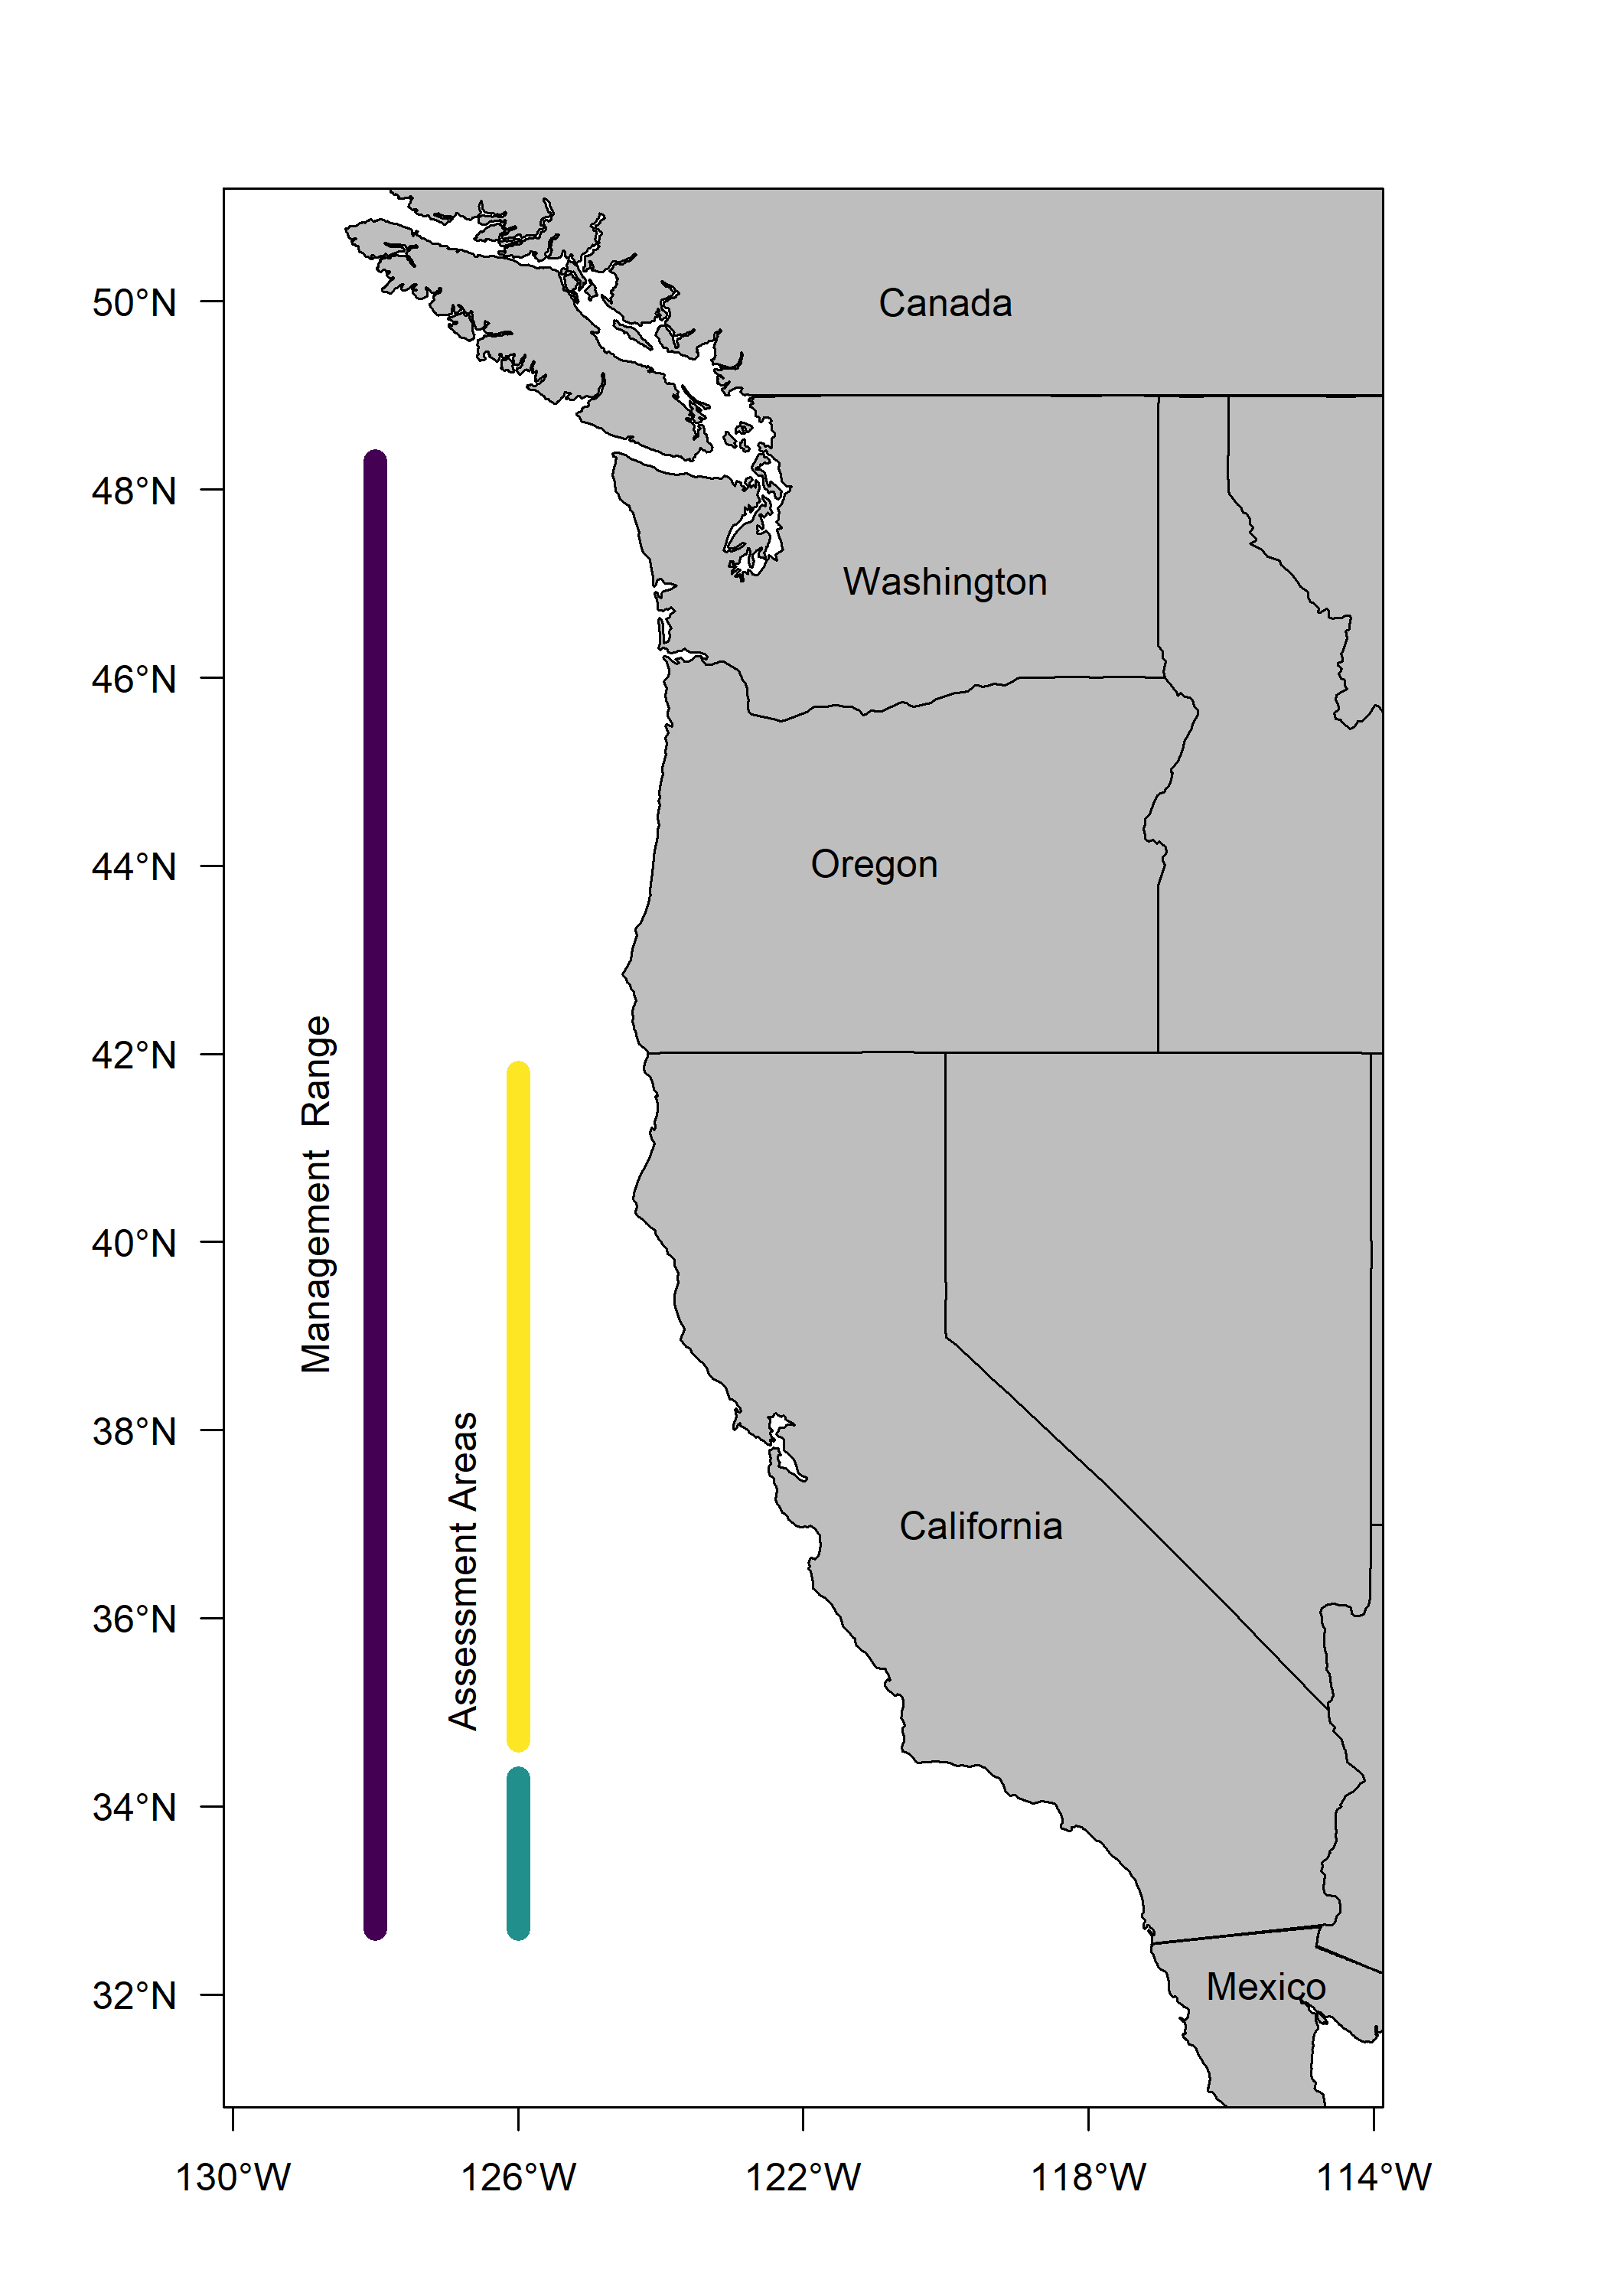
\includegraphics[width=1\textwidth,height=1\textheight]{C:/Users/melissa.monk/Documents/GitHub/copper_rockfish_2023/documents/shared_figures/map.png}
\caption{Map of management area and the 2023 assessments areas for copper rockfish.\label{fig:ca-map}}
\end{figure}

\begin{figure}
\centering
\includegraphics[width=1\textwidth,height=1\textheight]{S:/copper_rockfish_2023/models/nca/8.5_update_deb_index/plots/catch2 landings stacked.png}
\caption{Landings by fleet used in the base model where catches in metric tons by fleet are stacked.\label{fig:catch}}
\end{figure}

\begin{figure}
\centering
\includegraphics[width=1\textwidth,height=1\textheight]{S:/copper_rockfish_2023/models/nca/8.5_update_deb_index/plots/data_plot.png}
\caption{Summary of data sources used in the base model.\label{fig:data-plot}}
\end{figure}

\begin{figure}
\centering
\includegraphics[width=1\textwidth,height=1\textheight]{S:/copper_rockfish_2023/models/nca/8.5_update_deb_index/plots/comp_lendat_bubflt1mkt0.png}
\caption{Length composition data from the commercial dead fleet.\label{fig:com-dead-len-data}}
\end{figure}

\begin{figure}
\centering
\includegraphics[width=1\textwidth,height=1\textheight]{S:/copper_rockfish_2023/models/nca/8.5_update_deb_index/plots/comp_lendat_data_weighting_TA1.8_Commercial_Dead.png}
\caption{Mean length for commercial dead fleet with 95 percent confidence intervals.\label{fig:mean-com-dead-len-data}}
\end{figure}

\begin{figure}
\centering
\includegraphics[width=1\textwidth,height=1\textheight]{S:/copper_rockfish_2023/models/nca/8.5_update_deb_index/plots/comp_condAALdat_bubflt1mkt0.png}
\caption{Conditional age-at-length composition data from the commercial dead fleet.\label{fig:com-dead-age-data}}
\end{figure}

\begin{figure}
\centering
\includegraphics[width=1\textwidth,height=1\textheight]{S:/copper_rockfish_2023/models/nca/8.5_update_deb_index/plots/comp_lendat_bubflt2mkt0.png}
\caption{Length composition data from the commercial live fleet.\label{fig:com-live-len-data}}
\end{figure}

\begin{figure}
\centering
\includegraphics[width=1\textwidth,height=1\textheight]{S:/copper_rockfish_2023/models/nca/8.5_update_deb_index/plots/comp_lendat_data_weighting_TA1.8_Commercial_Live.png}
\caption{Mean length for commercial live fleet with 95 percent confidence intervals.\label{fig:mean-com-live-len-data}}
\end{figure}

\begin{figure}
\centering
\includegraphics[width=1\textwidth,height=1\textheight]{S:/copper_rockfish_2023/data/rec_indices/mrfss_cpfv_dockside/north/forSS/Index.png}
\caption{Estimated annual index of abundances for the CPFV fleet based on MRFSS survey data.\label{fig:mrfss-index-main}}
\end{figure}

\begin{figure}
\centering
\includegraphics[width=1\textwidth,height=1\textheight]{S:/copper_rockfish_2023/data/rec_indices/debwv_cpfv_onboard/delta_lognormal_main_effects/Index.png}
\caption{Estimated annual index of abundances for the CPFV fleet based on the Deb Wilson-Vandenberg survey data.\label{fig:dwv-index-main}}
\end{figure}

\begin{figure}
\centering
\includegraphics[width=1\textwidth,height=1\textheight]{S:/copper_rockfish_2023/data/rec_indices/crfs_cpfv_onboard/north/area_weighted/Index.png}
\caption{Estimated annual index of abundances for the CPFV fleet based on CRFS survey data.\label{fig:crfs-index-main}}
\end{figure}

\begin{figure}
\centering
\includegraphics[width=1\textwidth,height=1\textheight]{S:/copper_rockfish_2023/data/rec_indices/crfs_pr_dockside/north/rm_last2yrs_area_weighted/Index.png}
\caption{Estimated annual index of abundances for the CPFV fleet based on CRFS survey data.\label{fig:crfs-pr-index-main}}
\end{figure}

\begin{figure}
\centering
\includegraphics[width=1\textwidth,height=1\textheight]{S:/copper_rockfish_2023/models/nca/8.5_update_deb_index/plots/comp_lendat_bubflt3mkt0_page2.png}
\caption{Length composition data from the recreational CPFV fleet.\label{fig:rec-cpfv-len-data}}
\end{figure}

\begin{figure}
\centering
\includegraphics[width=1\textwidth,height=1\textheight]{S:/copper_rockfish_2023/models/nca/8.5_update_deb_index/plots/comp_lendat_data_weighting_TA1.8_Rec_CPFV.png}
\caption{Mean length for recreational CPFV fleet with 95 percent confidence intervals.\label{fig:mean-rec-cpfv-len-data}}
\end{figure}

\begin{figure}
\centering
\includegraphics[width=1\textwidth,height=1\textheight]{S:/copper_rockfish_2023/models/nca/8.5_update_deb_index/plots/comp_condAALdat_bubflt3mkt0.png}
\caption{Conditional age-at-length composition data from the recreational CPFV fleet.\label{fig:rec-cpfv-caal-data}}
\end{figure}

\begin{figure}
\centering
\includegraphics[width=1\textwidth,height=1\textheight]{S:/copper_rockfish_2023/models/nca/8.5_update_deb_index/plots/comp_agedat_data_weighting_TA1.8_Rec_CPFV.png}
\caption{Mean age for recreational CPFV fleet with 95 percent confidence intervals.\label{fig:mean-rec-cpfv-age-data}}
\end{figure}

\begin{figure}
\centering
\includegraphics[width=1\textwidth,height=1\textheight]{S:/copper_rockfish_2023/data/ages/plots/coop_crfs_length_comparison.png}
\caption{Comparison of all length collected by the CRFS sampling program for the CPFV fleet to the lengths from the fish with ages from the cooperative sampling program. The length distributions in the area north of Point Conception are in general agreement while the distribution of lengths collected by this program does not align with the length samples from CRFS.\label{fig:coop-len-comparison}}
\end{figure}

\begin{figure}
\centering
\includegraphics[width=1\textwidth,height=1\textheight]{S:/copper_rockfish_2023/models/nca/8.5_update_deb_index/plots/comp_condAALdat_bubflt4mkt0.png}
\caption{Conditional age-at-length data for recreational PR collected in 2022.\label{fig:rec-pr-caal-data}}
\end{figure}

\begin{figure}
\centering
\includegraphics[width=1\textwidth,height=1\textheight]{S:/copper_rockfish_2023/models/nca/8.5_update_deb_index/plots/comp_lendat_flt4mkt0_page2.png}
\caption{Length composition data from the recreational PR fleet.\label{fig:rec-pr-len-data}}
\end{figure}

\begin{figure}
\centering
\includegraphics[width=1\textwidth,height=1\textheight]{S:/copper_rockfish_2023/models/nca/8.5_update_deb_index/plots/comp_lendat_data_weighting_TA1.8_Rec_PR.png}
\caption{Mean length for recreational PR fleet with 95 percent confidence intervals.\label{fig:mean-rec-pr-len-data}}
\end{figure}

\begin{figure}
\centering
\includegraphics[width=1\textwidth,height=1\textheight]{S:/copper_rockfish_2023/data/survey_indices/plots/north_survey_locations_designation.png}
\caption{Sample locations by each of the fishery-independent data sources used in the base model with indices of abundance, lengths, and ages if collected.\label{fig:survey-locations}}
\end{figure}

\begin{figure}
\centering
\includegraphics[width=1\textwidth,height=1\textheight]{S:/copper_rockfish_2023/data/survey_indices/plots/north_survey_locations.png}
\caption{Sample locations by area, areas open to fishing (reference) and MPAS, for each of the fishery-independent data sources used in the base model with indices of abundance, lengths, and ages if collected.\label{fig:ref-mpa}}
\end{figure}

\begin{figure}
\centering
\includegraphics[width=1\textwidth,height=1\textheight]{S:/copper_rockfish_2023/data/survey_indices/ccfrp/north/area_weighted/Index.png}
\caption{Estimated index of abundance from the CCFRP survey.\label{fig:ccfrp-index-main}}
\end{figure}

\begin{figure}
\centering
\includegraphics[width=1\textwidth,height=1\textheight]{S:/copper_rockfish_2023/models/nca/8.5_update_deb_index/plots/comp_lendat_bubflt5mkt0.png}
\caption{Length composition data from the CCFRP survey.\label{fig:ccfrp-len-data}}
\end{figure}

\begin{figure}
\centering
\includegraphics[width=1\textwidth,height=1\textheight]{S:/copper_rockfish_2023/models/nca/8.5_update_deb_index/plots/comp_lendat_data_weighting_TA1.8_CCFRP.png}
\caption{Mean length for the CCFRP survey with 95 percent confidence intervals.\label{fig:ccfrp-mean-len-data}}
\end{figure}

\begin{figure}
\centering
\includegraphics[width=1\textwidth,height=1\textheight]{S:/copper_rockfish_2023/models/nca/8.5_update_deb_index/plots/comp_condAALdat_bubflt5mkt0.png}
\caption{Conditional age-at-length data from the CCFRP survey.\label{fig:ccfrp-age-data}}
\end{figure}

\begin{figure}
\centering
\includegraphics[width=1\textwidth,height=1\textheight]{S:/copper_rockfish_2023/data/survey_indices/rov/plots/rov_transect_collapsed_copper_north_protection_count.png}
\caption{The location and size of observations across all years and transects.\label{fig:rov-obs-loc}}
\end{figure}

\begin{figure}
\centering
\includegraphics[width=1\textwidth,height=1\textheight]{S:/copper_rockfish_2023/data/survey_indices/rov/plots/north_raw_cpue_by_mpa_group.png}
\caption{The trend of the calculated CPUE by each MPA and Reference group.\label{fig:rov-raw-cpue}}
\end{figure}

\begin{figure}
\centering
\includegraphics[width=1\textwidth,height=1\textheight]{S:/copper_rockfish_2023/data/survey_indices/rov/glm_negbin_north_designation_depth/Index.png}
\caption{The estimated weighted relative index of abundance.\label{fig:rov-index-main}}
\end{figure}

\begin{figure}
\centering
\includegraphics[width=1\textwidth,height=1\textheight]{S:/copper_rockfish_2023/data/survey_indices/rov/plots/rov_length_by_area_designation.png}
\caption{The distribution of lengths across all years for MPA and Reference area north and south of Point Conception.\label{fig:rov-len}}
\end{figure}

\begin{figure}
\centering
\includegraphics[width=1\textwidth,height=1\textheight]{S:/copper_rockfish_2023/models/nca/8.5_update_deb_index/plots/comp_lendat_flt6mkt0.png}
\caption{Length composition data from the CDFW ROV survey.\label{fig:rov-len-data}}
\end{figure}

\begin{figure}
\centering
\includegraphics[width=1\textwidth,height=1\textheight]{S:/copper_rockfish_2023/models/nca/8.5_update_deb_index/plots/comp_lendat_data_weighting_TA1.8_CDFW_ROV.png}
\caption{Mean length for CDWF ROV survey with 95 percent confidence intervals.\label{fig:mean-rov-len-data}}
\end{figure}

\begin{figure}
\centering
\includegraphics[width=1\textwidth,height=1\textheight]{S:/copper_rockfish_2023/data/ages/plots/south_growth_length_comparison.png}
\caption{Length distribution of fish by collection source that were used as conditional age-at-length data in the growth fleet.\label{fig:growth-len-dist}}
\end{figure}

\begin{figure}
\centering
\includegraphics[width=1\textwidth,height=1\textheight]{S:/copper_rockfish_2023/data/ages/plots/south_growth_age_comparison.png}
\caption{Age distribution of fish by collection source that were used as conditional age-at-length data in the growth fleet.\label{fig:growth-age-dist}}
\end{figure}

\begin{figure}
\centering
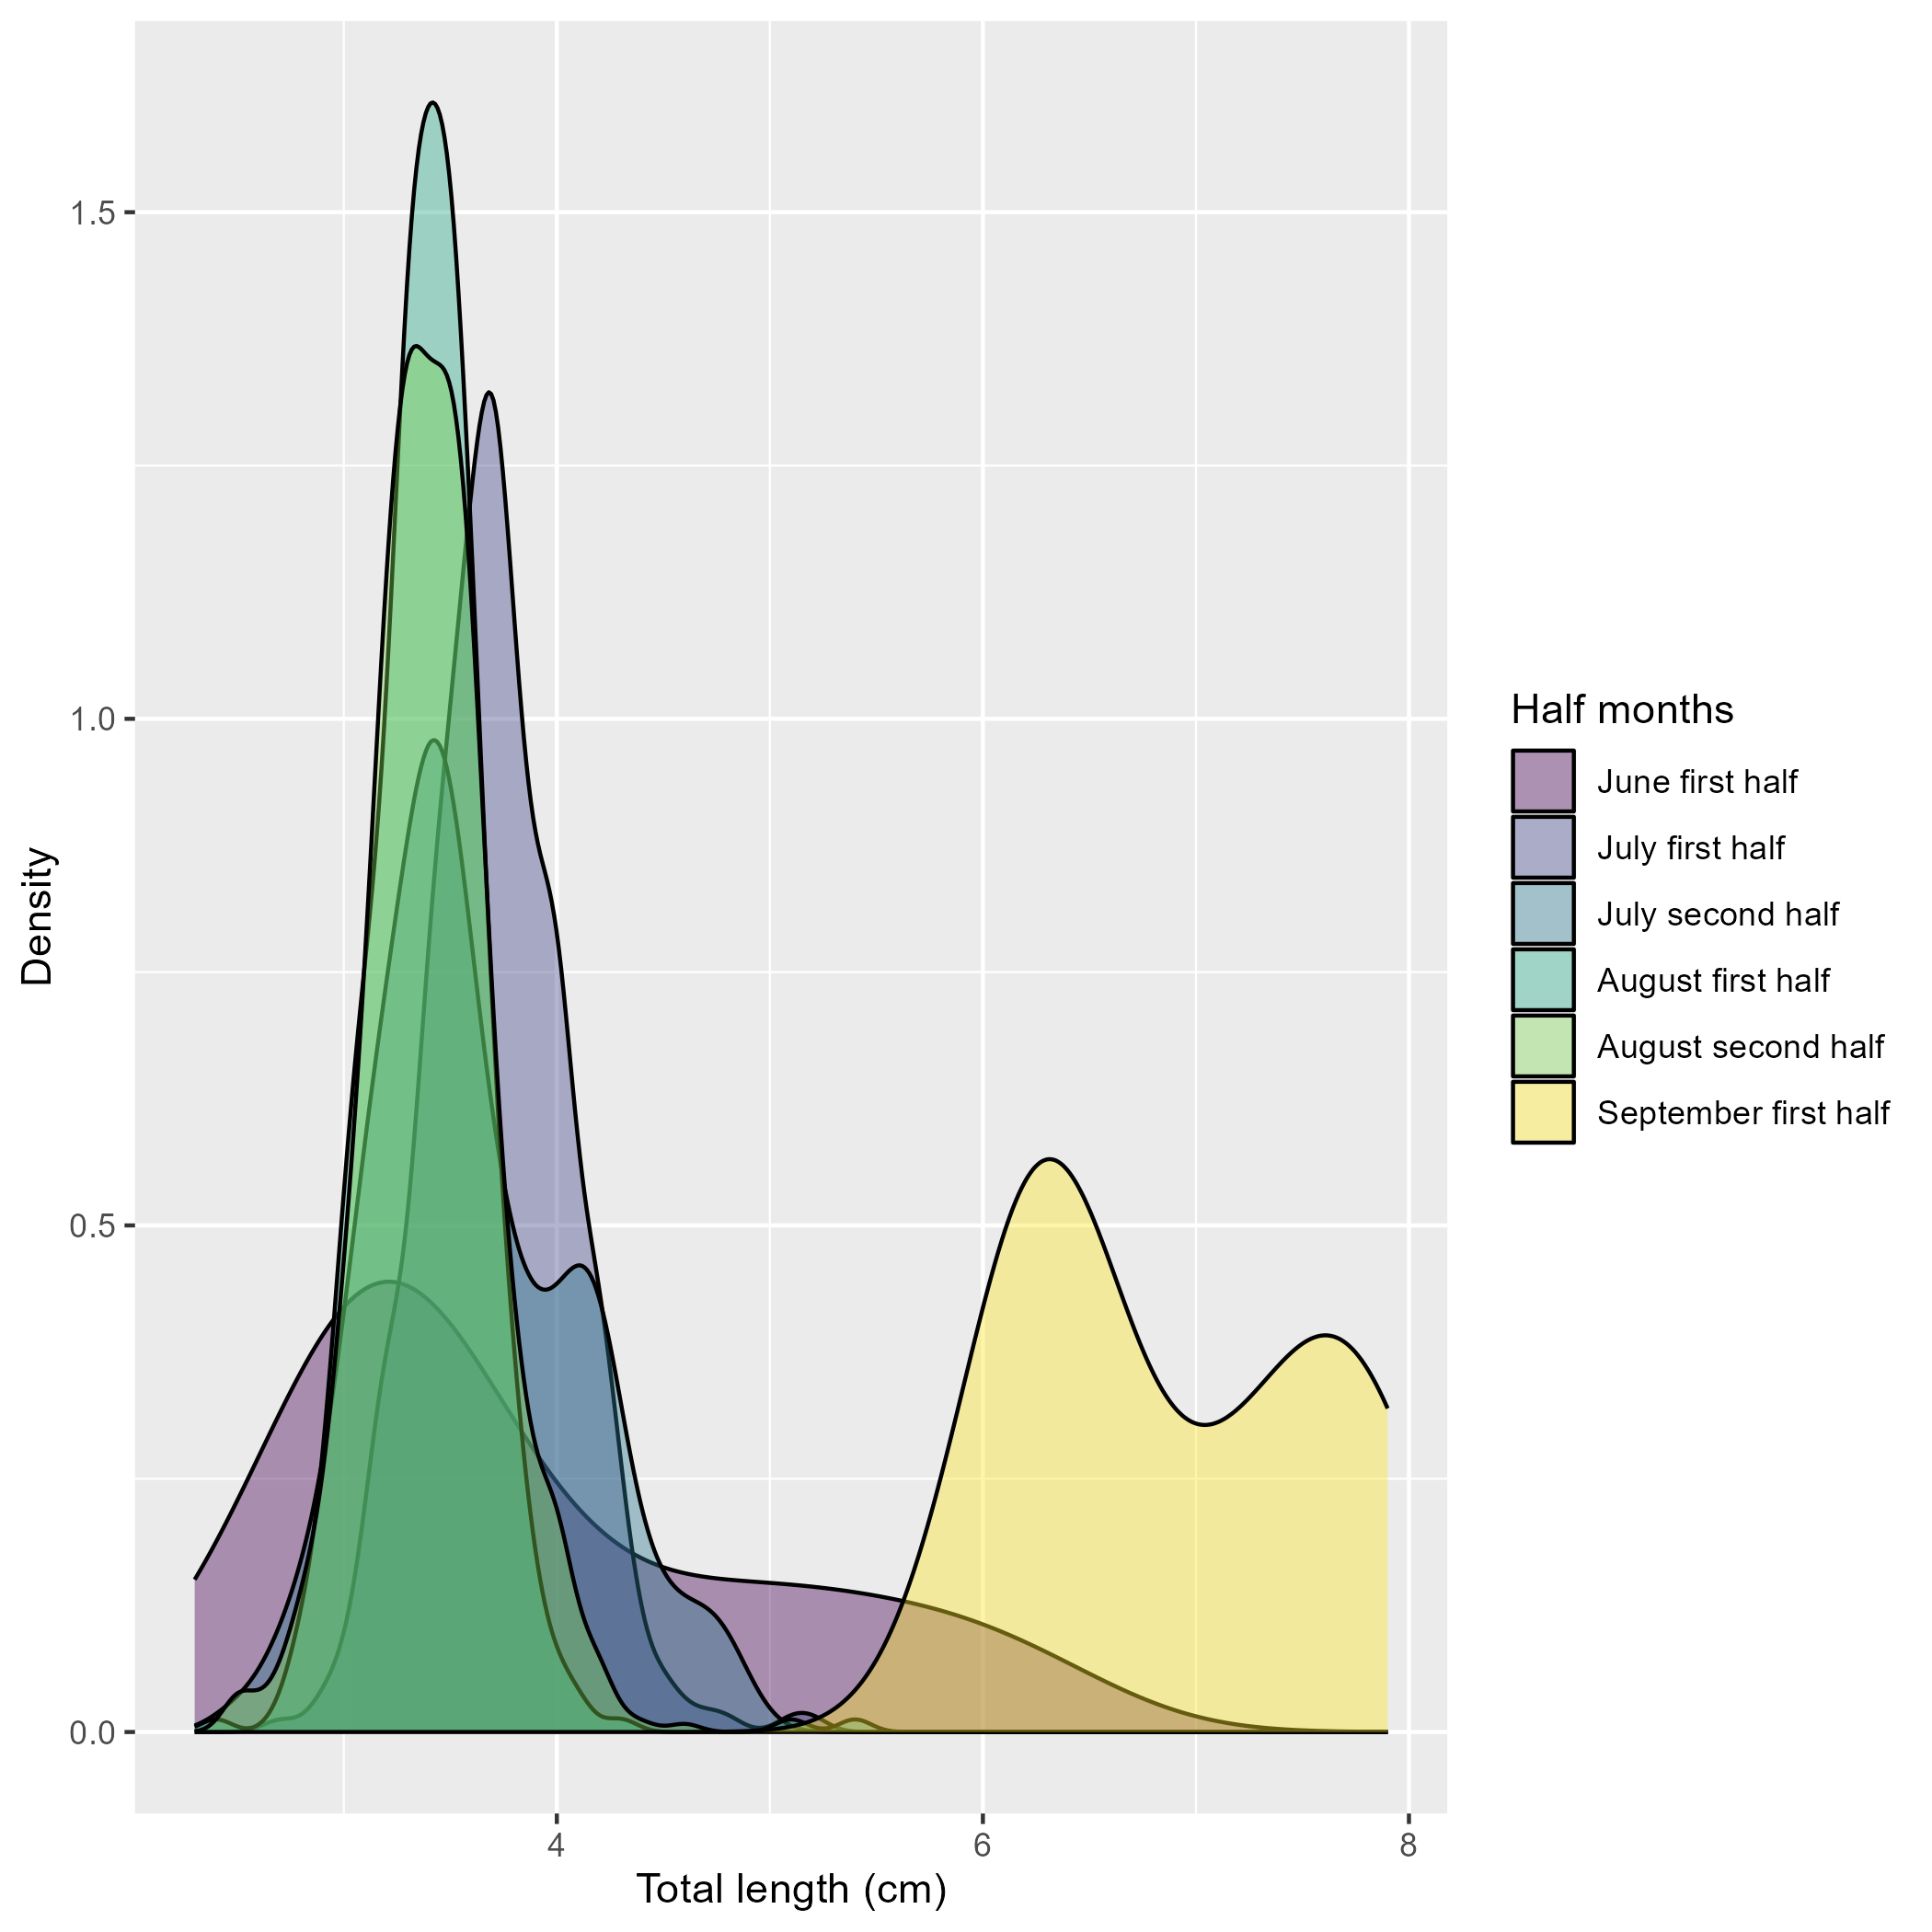
\includegraphics[width=1\textwidth,height=1\textheight]{C:/Users/melissa.monk/Documents/GitHub/copper_rockfish_2023/documents/shared_figures/copper_length_by_half_month.png}
\caption{Distribution of YOY copper rockfish lengths from fish genetically identified from D. Baetscher.\label{fig:copper-smurf-length}}
\end{figure}

\begin{figure}
\centering
\includegraphics[width=1\textwidth,height=1\textheight]{S:/copper_rockfish_2023/models/nca/8.5_update_deb_index/plots/bio6_maturity.png}
\caption{Maturity as a function of length.\label{fig:maturity}}
\end{figure}

\begin{figure}
\centering
\includegraphics[width=1\textwidth,height=1\textheight]{S:/copper_rockfish_2023/models/nca/8.5_update_deb_index/plots/bio9_fecundity_len.png}
\caption{Fecundity as a function of length.\label{fig:fecundity}}
\end{figure}

\begin{figure}
\centering
\includegraphics[width=1\textwidth,height=1\textheight]{S:/copper_rockfish_2023/data/wcgbt/plots/length_fraction_female.png}
\caption{Fraction of each sex by length by the NWFSC WCGBT survey.\label{fig:frac-sex-len}}
\end{figure}

\begin{figure}
\centering
\includegraphics[width=1\textwidth,height=1\textheight]{S:/copper_rockfish_2023/data/biology/plots/Length_Weight_All.png}
\caption{Estimated weight-at-length.\label{fig:weight-length}}
\end{figure}

\begin{figure}
\centering
\includegraphics[width=1\textwidth,height=1\textheight]{S:/copper_rockfish_2023/data/ages/ageing_error/B0_S3/Reader_1_vs_Reader_2.png}
\caption{Distribution of double reads between age reader 1 and 2.\label{fig:age-error-dist}}
\end{figure}

\begin{figure}
\centering
\includegraphics[width=1\textwidth,height=1\textheight]{S:/copper_rockfish_2023/models/nca/8.5_update_deb_index/plots/numbers5_ageerrorSD.png}
\caption{Ageing imprecision standard deviation of observed age in years.\label{fig:age-error}}
\end{figure}

\begin{figure}
\centering
\includegraphics[width=1\textwidth,height=1\textheight]{S:/copper_rockfish_2023/models/nca/8.5_update_deb_index/plots/numbers10_ageerror_matrix_1.png}
\caption{Distribution of observed age at true age for ageing error type 1.\label{fig:age-error-matrix}}
\end{figure}

\begin{figure}
\centering
\includegraphics[width=1\textwidth,height=1\textheight]{S:/copper_rockfish_2023/models/nca/_bridging/_plots/0_model_convert_compare2_spawnbio_uncertainty.png}
\caption{Model version bridge comparison of estimated spawning output.\label{fig:bridge-ssb}}
\end{figure}

\begin{figure}
\centering
\includegraphics[width=1\textwidth,height=1\textheight]{S:/copper_rockfish_2023/models/nca/_bridging/_plots/0_model_convert_compare4_Bratio_uncertainty.png}
\caption{Model version bridge comparison of estimated fraction unfished.\label{fig:bridge-depl}}
\end{figure}

\begin{figure}
\centering
\includegraphics[width=1\textwidth,height=1\textheight]{S:/copper_rockfish_2023/models/nca/_bridging/_plots/full_bridge_1_compare2_spawnbio_uncertainty.png}
\caption{Model structure and data bridging comparison of estimated spawning output.\label{fig:data-bridge-ssb-1}}
\end{figure}

\begin{figure}
\centering
\includegraphics[width=1\textwidth,height=1\textheight]{S:/copper_rockfish_2023/models/nca/_bridging/_plots/full_bridge_1_compare4_Bratio_uncertainty.png}
\caption{Model structure and data bridging comparison of estimated fraction unfished.\label{fig:data-bridge-depl-1}}
\end{figure}

\begin{figure}
\centering
\includegraphics[width=1\textwidth,height=1\textheight]{S:/copper_rockfish_2023/models/nca/_bridging/_plots/full_bridge_2_compare2_spawnbio_uncertainty.png}
\caption{Model structure and data bridging comparison of estimated spawning output.\label{fig:data-bridge-ssb-2}}
\end{figure}

\begin{figure}
\centering
\includegraphics[width=1\textwidth,height=1\textheight]{S:/copper_rockfish_2023/models/nca/_bridging/_plots/full_bridge_2_compare4_Bratio_uncertainty.png}
\caption{Model structure and data bridging comparison of estimated fraction unfished.\label{fig:data-bridge-depl-2}}
\end{figure}

\begin{figure}
\centering
\includegraphics[width=1\textwidth,height=1\textheight]{S:/copper_rockfish_2023/models/nca/8.5_update_deb_index/plots/bio1_sizeatage.png}
\caption{Model estimated length-at-age in the beginning of the year. Shaded area indicates 95 percent distribution of length-at-age around the estimated growth curve.\label{fig:mod-est-len-age}}
\end{figure}

\begin{figure}
\centering
\includegraphics[width=1\textwidth,height=1\textheight]{S:/copper_rockfish_2023/models/nca/8.5_update_deb_index/plots/ts11_Age-0_recruits_(1000s)_with_95_asymptotic_intervals.png}
\caption{Estimated time series of age-0 recruits (1000s).\label{fig:recruits}}
\end{figure}

\begin{figure}
\centering
\includegraphics[width=1\textwidth,height=1\textheight]{S:/copper_rockfish_2023/models/nca/8.5_update_deb_index/plots/recdevs2_withbars.png}
\caption{Estimated time series of recruitment deviations.\label{fig:rec-devs}}
\end{figure}

\begin{figure}
\centering
\includegraphics[width=1\textwidth,height=1\textheight]{S:/copper_rockfish_2023/models/nca/8.5_update_deb_index/plots/SR_curve.png}
\caption{Stock-recruit curve. Point colors indicate year, with warmer colors indicating earlier years and cooler colors in showing later years.\label{fig:bh-curve}}
\end{figure}

\begin{figure}
\centering
\includegraphics[width=1\textwidth,height=1\textheight]{S:/copper_rockfish_2023/models/nca/8.5_update_deb_index/plots/index5_logcpuefit_Rec_CPFV.png}
\caption{Fit to log index data on log scale for recreational (MRFSS) CPFV. Lines indicate 95\% uncertainty interval around index values based on the model assumption of lognormal error. Thicker lines (if present) indicate input uncertainty before addition of estimated additional uncertainty parameter.\label{fig:mrfss-cpfv-index-fit}}
\end{figure}

\begin{figure}
\centering
\includegraphics[width=1\textwidth,height=1\textheight]{S:/copper_rockfish_2023/models/nca/8.5_update_deb_index/plots/index5_logcpuefit_DWV_CPFV.png}
\caption{Fit to log index data on log scale for Deb Wilson-Vandenberg CPFV survey. Lines indicate 95\% uncertainty interval around index values based on the model assumption of lognormal error. Thicker lines (if present) indicate input uncertainty before addition of estimated additional uncertainty parameter.\label{fig:dwv-cpfv-index-fit}}
\end{figure}

\begin{figure}
\centering
\includegraphics[width=1\textwidth,height=1\textheight]{S:/copper_rockfish_2023/models/nca/8.5_update_deb_index/plots/index5_logcpuefit_CRFS_CPFV.png}
\caption{Fit to log index data on log scale for CRFS CPFV survey. Lines indicate 95\% uncertainty interval around index values based on the model assumption of lognormal error. Thicker lines (if present) indicate input uncertainty before addition of estimated additional uncertainty parameter.\label{fig:crfs-cpfv-index-fit}}
\end{figure}

\begin{figure}
\centering
\includegraphics[width=1\textwidth,height=1\textheight]{S:/copper_rockfish_2023/models/nca/8.5_update_deb_index/plots/index5_logcpuefit_Rec_PR.png}
\caption{Fit to log index data on log scale for recreational (CRFS) PR. Lines indicate 95\% uncertainty interval around index values based on the model assumption of lognormal error. Thicker lines (if present) indicate input uncertainty before addition of estimated additional uncertainty parameter.\label{fig:crfs-pr-index-fit}}
\end{figure}

\begin{figure}
\centering
\includegraphics[width=1\textwidth,height=1\textheight]{S:/copper_rockfish_2023/models/nca/8.5_update_deb_index/plots/index5_logcpuefit_CCFRP.png}
\caption{Fit to log index data on log scale for CCFRP survey. Lines indicate 95\% uncertainty interval around index values based on the model assumption of lognormal error. Thicker lines (if present) indicate input uncertainty before addition of estimated additional uncertainty parameter.\label{fig:ccfrp-index-fit}}
\end{figure}

\begin{figure}
\centering
\includegraphics[width=1\textwidth,height=1\textheight]{S:/copper_rockfish_2023/models/nca/8.5_update_deb_index/plots/index5_logcpuefit_CDFW_ROV.png}
\caption{Fit to log index data on log scale for CDFW ROV survey. Lines indicate 95\% uncertainty interval around index values based on the model assumption of lognormal error. Thicker lines (if present) indicate input uncertainty before addition of estimated additional uncertainty parameter.\label{fig:rov-index-fit}}
\end{figure}

\begin{figure}
\centering
\includegraphics[width=1\textwidth,height=1\textheight]{S:/copper_rockfish_2023/models/nca/8.5_update_deb_index/plots/index9_standcpueall.png}
\caption{Standardized indices overlaid. Each index is rescaled to have mean observation = 1.0.\label{fig:standardized-indices}}
\end{figure}

\begin{figure}
\centering
\includegraphics[width=1\textwidth,height=1\textheight]{S:/copper_rockfish_2023/models/nca/8.5_update_deb_index/plots/ts7_Spawning_output_with_95_asymptotic_intervals_intervals.png}
\caption{Estimated time series of spawning biomass.\label{fig:ssb}}
\end{figure}

\begin{figure}
\centering
\includegraphics[width=1\textwidth,height=1\textheight]{S:/copper_rockfish_2023/models/nca/8.5_update_deb_index/plots/ts1_Total_biomass_(mt).png}
\caption{Estimated time series of total biomass.\label{fig:tot-bio}}
\end{figure}

\begin{figure}
\centering
\includegraphics[width=1\textwidth,height=1\textheight]{S:/copper_rockfish_2023/models/nca/8.5_update_deb_index/plots/ts9_Relative_spawning_output_intervals.png}
\caption{Estimated time series of fraction of unfished spawning biomass.\label{fig:depl}}
\end{figure}

\begin{figure}
\centering
\includegraphics[width=1\textwidth,height=1\textheight]{S:/copper_rockfish_2023/models/nca/8.5_update_deb_index/plots/SPR2_minusSPRseries.png}
\caption{Estimated 1 - relative spawning ratio (SPR) by year.\label{fig:1-spr}}
\end{figure}

\clearpage

\begin{figure}
\centering
\includegraphics[width=1\textwidth,height=1\textheight]{S:/copper_rockfish_2023/models/nca/8.5_update_deb_index/plots/SPR4_phase.png}
\caption{Phase plot of the relative biomass (also referred to as fraction unfished) versus the SPR ratio where each point represents the biomass ratio at the start of the year and the relative fishing intensity in that same year. Lines through the final point show the 95 percent intervals based on the asymptotic uncertainty for each dimension. The shaded ellipse is a 95 percent region which accounts for the estimated correlations between the biomass ratio and SPR ratio.\label{fig:phase}}
\end{figure}

\begin{figure}
\centering
\includegraphics[width=1\textwidth,height=1\textheight]{S:/copper_rockfish_2023/models/nca/8.5_update_deb_index/plots/yield2_yield_curve_with_refpoints.png}
\caption{Equilibrium yield curve for the base case model. Values are based on the 2022 fishery selectivities and with steepness fixed at 0.72.\label{fig:yield}}
\end{figure}

\hypertarget{detailed-fit-comps}{%
\section{Appendix A}\label{detailed-fit-comps}}

\hypertarget{length-data}{%
\subsection{Detailed Fit to Length Composition Data}\label{length-data}}

\begin{figure}
\centering
\includegraphics[width=1\textwidth,height=1\textheight]{S:/copper_rockfish_2023/models/nca/8.5_update_deb_index/plots/comp_lenfit_flt1mkt0.png}
\caption{Length comps, whole catch, Commercial\_Dead.`N adj.' is the input sample size after data-weighting adjustment. N eff. is the calculated effective sample size used in the McAllister-Ianelli tuning method.\label{fig:comp_lenfit_flt1mkt0}}
\end{figure}

\begin{figure}
\centering
\includegraphics[width=1\textwidth,height=1\textheight]{S:/copper_rockfish_2023/models/nca/8.5_update_deb_index/plots/comp_lenfit_flt2mkt0.png}
\caption{Length comps, whole catch, Commercial\_Live.`N adj.' is the input sample size after data-weighting adjustment. N eff. is the calculated effective sample size used in the McAllister-Ianelli tuning method.\label{fig:comp_lenfit_flt2mkt0}}
\end{figure}

\begin{figure}
\centering
\includegraphics[width=1\textwidth,height=1\textheight]{S:/copper_rockfish_2023/models/nca/8.5_update_deb_index/plots/comp_lenfit_flt3mkt0_page1.png}
\caption{Length comps, whole catch, Rec\_CPFV (plot 1 of 2).`N adj.' is the input sample size after data-weighting adjustment. N eff. is the calculated effective sample size used in the McAllister-Ianelli tuning method.\label{fig:comp_lenfit_flt3mkt0_page1}}
\end{figure}

\begin{figure}
\centering
\includegraphics[width=1\textwidth,height=1\textheight]{S:/copper_rockfish_2023/models/nca/8.5_update_deb_index/plots/comp_lenfit_flt3mkt0_page2.png}
\caption{Length comps, whole catch, Rec\_CPFV (plot 1 of 2).`N adj.' is the input sample size after data-weighting adjustment. N eff. is the calculated effective sample size used in the McAllister-Ianelli tuning method. (plot 2 of 2).\label{fig:comp_lenfit_flt3mkt0_page2}}
\end{figure}

\begin{figure}
\centering
\includegraphics[width=1\textwidth,height=1\textheight]{S:/copper_rockfish_2023/models/nca/8.5_update_deb_index/plots/comp_lenfit_flt4mkt0_page1.png}
\caption{Length comps, whole catch, Rec\_PR (plot 1 of 2).`N adj.' is the input sample size after data-weighting adjustment. N eff. is the calculated effective sample size used in the McAllister-Ianelli tuning method.\label{fig:comp_lenfit_flt4mkt0_page1}}
\end{figure}

\begin{figure}
\centering
\includegraphics[width=1\textwidth,height=1\textheight]{S:/copper_rockfish_2023/models/nca/8.5_update_deb_index/plots/comp_lenfit_flt4mkt0_page2.png}
\caption{Length comps, whole catch, Rec\_PR (plot 1 of 2).`N adj.' is the input sample size after data-weighting adjustment. N eff. is the calculated effective sample size used in the McAllister-Ianelli tuning method. (plot 2 of 2).\label{fig:comp_lenfit_flt4mkt0_page2}}
\end{figure}

\begin{figure}
\centering
\includegraphics[width=1\textwidth,height=1\textheight]{S:/copper_rockfish_2023/models/nca/8.5_update_deb_index/plots/comp_lenfit_flt5mkt0.png}
\caption{Length comps, whole catch, CCFRP.`N adj.' is the input sample size after data-weighting adjustment. N eff. is the calculated effective sample size used in the McAllister-Ianelli tuning method.\label{fig:comp_lenfit_flt5mkt0}}
\end{figure}

\begin{figure}
\centering
\includegraphics[width=1\textwidth,height=1\textheight]{S:/copper_rockfish_2023/models/nca/8.5_update_deb_index/plots/comp_lenfit_flt6mkt0.png}
\caption{Length comps, whole catch, CDFW\_ROV.`N adj.' is the input sample size after data-weighting adjustment. N eff. is the calculated effective sample size used in the McAllister-Ianelli tuning method.\label{fig:comp_lenfit_flt6mkt0}}
\end{figure}

\newpage

\hypertarget{age-data}{%
\subsection{Detailed Fit to Age Composition Data}\label{age-data}}

\newpage

\hypertarget{caal-data}{%
\subsection{Detailed Fit to Conditional-Age-at-Length Composition Data}\label{caal-data}}

\begin{figure}
\centering
\includegraphics[width=1\textwidth,height=1\textheight]{S:/copper_rockfish_2023/models/nca/8.5_update_deb_index/plots/comp_condAALfit_residsflt9mkt0_page1.png}
\caption{Pearson residuals, whole catch, Growth (max=33.43) (plot 1 of 4).\label{fig:comp_condAALfit_residsflt9mkt0_page1}}
\end{figure}

\begin{figure}
\centering
\includegraphics[width=1\textwidth,height=1\textheight]{S:/copper_rockfish_2023/models/nca/8.5_update_deb_index/plots/comp_condAALfit_residsflt9mkt0_page2.png}
\caption{Pearson residuals, whole catch, Growth (max=33.43) (plot 2 of 4).\label{fig:comp_condAALfit_residsflt9mkt0_page2}}
\end{figure}

\begin{figure}
\centering
\includegraphics[width=1\textwidth,height=1\textheight]{S:/copper_rockfish_2023/models/nca/8.5_update_deb_index/plots/comp_condAALfit_residsflt9mkt0_page3.png}
\caption{Pearson residuals, whole catch, Growth (max=33.43) (plot 3 of 4).\label{fig:comp_condAALfit_residsflt9mkt0_page3}}
\end{figure}

\begin{figure}
\centering
\includegraphics[width=1\textwidth,height=1\textheight]{S:/copper_rockfish_2023/models/nca/8.5_update_deb_index/plots/comp_condAALfit_residsflt9mkt0_page4.png}
\caption{Pearson residuals, whole catch, Growth (max=33.43) (plot 4 of 4).\label{fig:comp_condAALfit_residsflt9mkt0_page4}}
\end{figure}

\begin{figure}
\centering
\includegraphics[width=1\textwidth,height=1\textheight]{S:/copper_rockfish_2023/models/nca/8.5_update_deb_index/plots/comp_condAALfit_Andre_plotsflt5mkt0.png}
\caption{Conditional AAL plot, whole catch, CCFRP These plots show mean age and std. dev. in conditional \href{mailto:A@L}{\nolinkurl{A@L}}.Left plots are mean \href{mailto:A@L}{\nolinkurl{A@L}} by size-class (obs. and exp.) with 90\% CIs based on adding 1.64 SE of mean to the data.Right plots in each pair are SE of mean \href{mailto:A@L}{\nolinkurl{A@L}} (obs. and exp.) with 90\% CIs based on the chi-square distribution.\label{fig:comp_condAALfit_Andre_plotsflt5mkt0}}
\end{figure}

\begin{figure}
\centering
\includegraphics[width=1\textwidth,height=1\textheight]{S:/copper_rockfish_2023/models/nca/8.5_update_deb_index/plots/comp_condAALfit_Andre_plotsflt9mkt0_page1.png}
\caption{Conditional AAL plot, whole catch, Growth (plot 1 of 6) These plots show mean age and std. dev. in conditional \href{mailto:A@L}{\nolinkurl{A@L}}.Left plots are mean \href{mailto:A@L}{\nolinkurl{A@L}} by size-class (obs. and exp.) with 90\% CIs based on adding 1.64 SE of mean to the data.Right plots in each pair are SE of mean \href{mailto:A@L}{\nolinkurl{A@L}} (obs. and exp.) with 90\% CIs based on the chi-square distribution.\label{fig:comp_condAALfit_Andre_plotsflt9mkt0_page1}}
\end{figure}

\begin{figure}
\centering
\includegraphics[width=1\textwidth,height=1\textheight]{S:/copper_rockfish_2023/models/nca/8.5_update_deb_index/plots/comp_condAALfit_Andre_plotsflt9mkt0_page2.png}
\caption{Conditional AAL plot, whole catch, Growth (plot 2 of 6).\label{fig:comp_condAALfit_Andre_plotsflt9mkt0_page2}}
\end{figure}

\begin{figure}
\centering
\includegraphics[width=1\textwidth,height=1\textheight]{S:/copper_rockfish_2023/models/nca/8.5_update_deb_index/plots/comp_condAALfit_Andre_plotsflt9mkt0_page3.png}
\caption{Conditional AAL plot, whole catch, Growth (plot 3 of 6).\label{fig:comp_condAALfit_Andre_plotsflt9mkt0_page3}}
\end{figure}

\begin{figure}
\centering
\includegraphics[width=1\textwidth,height=1\textheight]{S:/copper_rockfish_2023/models/nca/8.5_update_deb_index/plots/comp_condAALfit_Andre_plotsflt9mkt0_page4.png}
\caption{Conditional AAL plot, whole catch, Growth (plot 4 of 6).\label{fig:comp_condAALfit_Andre_plotsflt9mkt0_page4}}
\end{figure}

\begin{figure}
\centering
\includegraphics[width=1\textwidth,height=1\textheight]{S:/copper_rockfish_2023/models/nca/8.5_update_deb_index/plots/comp_condAALfit_Andre_plotsflt9mkt0_page5.png}
\caption{Conditional AAL plot, whole catch, Growth (plot 5 of 6).\label{fig:comp_condAALfit_Andre_plotsflt9mkt0_page5}}
\end{figure}

\begin{figure}
\centering
\includegraphics[width=1\textwidth,height=1\textheight]{S:/copper_rockfish_2023/models/nca/8.5_update_deb_index/plots/comp_condAALfit_Andre_plotsflt9mkt0_page6.png}
\caption{Conditional AAL plot, whole catch, Growth (plot 6 of 6).\label{fig:comp_condAALfit_Andre_plotsflt9mkt0_page6}}
\end{figure}

\hypertarget{excluded-data}{%
\subsection{Implied Fit to Excluded Length Data}\label{excluded-data}}

The implied fits to the data not included in the base model due to low annual sample size are shown below.

\begin{figure}
\centering
\includegraphics[width=1\textwidth,height=1\textheight]{S:/copper_rockfish_2023/models/nca/8.5_update_deb_index/plots/comp_gstlenfit_flt1mkt0_page1.png}
\caption{Excluded length comps, whole catch, Commercial\_Dead (plot 1 of 2).`N adj.' is the input sample size after data-weighting adjustment. N eff. is the calculated effective sample size used in the McAllister-Ianelli tuning method.\label{fig:comp_gstlenfit_flt1mkt0_page1}}
\end{figure}

\begin{figure}
\centering
\includegraphics[width=1\textwidth,height=1\textheight]{S:/copper_rockfish_2023/models/nca/8.5_update_deb_index/plots/comp_gstlenfit_flt1mkt0_page2.png}
\caption{Excluded length comps, whole catch, Commercial\_Dead (plot 1 of 2).`N adj.' is the input sample size after data-weighting adjustment. N eff. is the calculated effective sample size used in the McAllister-Ianelli tuning method. (plot 2 of 2).\label{fig:comp_gstlenfit_flt1mkt0_page2}}
\end{figure}

\begin{figure}
\centering
\includegraphics[width=1\textwidth,height=1\textheight]{S:/copper_rockfish_2023/models/nca/8.5_update_deb_index/plots/comp_gstlenfit_flt2mkt0.png}
\caption{Excluded length comps, whole catch, Commercial\_Live.`N adj.' is the input sample size after data-weighting adjustment. N eff. is the calculated effective sample size used in the McAllister-Ianelli tuning method.\label{fig:comp_gstlenfit_flt2mkt0}}
\end{figure}

\begin{figure}
\centering
\includegraphics[width=1\textwidth,height=1\textheight]{S:/copper_rockfish_2023/models/nca/8.5_update_deb_index/plots/comp_gstlenfit_flt3mkt0.png}
\caption{Excluded length comps, whole catch, Rec\_CPFV.`N adj.' is the input sample size after data-weighting adjustment. N eff. is the calculated effective sample size used in the McAllister-Ianelli tuning method.\label{fig:comp_gstlenfit_flt3mkt0}}
\end{figure}

\begin{figure}
\centering
\includegraphics[width=1\textwidth,height=1\textheight]{S:/copper_rockfish_2023/models/nca/8.5_update_deb_index/plots/comp_gstlenfit_flt4mkt0.png}
\caption{Excluded length comps, whole catch, Rec\_PR.`N adj.' is the input sample size after data-weighting adjustment. N eff. is the calculated effective sample size used in the McAllister-Ianelli tuning method.\label{fig:comp_gstlenfit_flt4mkt0}}
\end{figure}

\newpage

\hypertarget{mrfss-cpfv-index}{%
\section{Appendix B. MRFSS CPFV Dockside Index of Abundance}\label{mrfss-cpfv-index}}

\hypertarget{onboard-cpfv-index}{%
\section{Appendix C. California Onboard CPFV Index of Abundance}\label{onboard-cpfv-index}}

\hypertarget{dwv-cpfv-index}{%
\section{Appendix D. Deb Wilson-Vandenberg Onboard CPFV Index of Abundance}\label{dwv-cpfv-index}}

\hypertarget{crfs-pr-index}{%
\section{Appendix E. CRFS PR Dockside Index of Abundance}\label{crfs-pr-index}}

\hypertarget{ccfrp-index}{%
\section{Appendix F. CCFRP Index of Abundance}\label{ccfrp-index}}

\textbf{California Collaborative Fisheries Research Program Index}

The California Collaborative Fisheries Research Program, \href{https://www.mlml.calstate.edu/ccfrp/}{CCFRP}, is a fishery-independent hook-and-line survey designed to monitor nearshore fish populations at a series of sampling locations both inside and adjacent to MPAs (Richard M. Starr et al. 2015; Wendt and Starr 2009). The CCFRP survey began in 2007 along the central coast of California and was designed in collaboration with academics, NMFS scientists and fishermen. From 2007-2016 the CCFRP project was focused on the central California coast, and has monitored four MPAs consistently. In 2017, the CCFRP expanded coastwide within California.\\
The index of abundance was developed from the four MPAs sampled consistently (Año Nuevo and Point Lobos by Moss Landing Marine Labs; Point Buchon and Piedras Blancas by Cal Poly).

The survey design for CCFRP consists 500 x 500 m cells both within and adjacent to each MPA. On any given survey day site cells are randomly selected within a stratum (MPA and/or reference cells). CPFVs are chartered for the survey and the fishing captain is allowed to search within the cell for a fishing location. During a sampling event, each cell is fished for a total of 30-45 minutes by volunteer anglers. Each fish encountered is recorded, measured, and can be linked back to a particular angler, and released (or descended to depth). CCFRP samples shallower depths to avoid barotrauma-induced mortality.\\
Starting in 2017, a subset of fish have been retained to collect otoliths and fin clips that provide needed biological information for nearshore species. For the index of abundance, CPUE was modeled at the level of the drift, similar to the fishery-dependent onboard observer survey described above.

\emph{CCFRP Index: Data Preparation, Filtering, and Sample Sizes}

The CCFRP data are quality controlled at the time they are key punched and little filtering was needed for the index. Cells not consistently sampled over time were excluded as well as cells that never encountered copper rockfish. The full dataset for northern California contained 8,770 drifts, 23\% of which encountered copper rockfish. After applying filters to remove drfits from sites that were not consistently sampled, marked for exclusion in the data, or did not fish a minimum of xxx, 7,078 drifts remained for for index standardization, with 1,757 drifts encountering copper rockfish.

\emph{CCFRP Index: Model Selection, Fits, and Diagnostics}

The CCFRP index includes all of the MPAs currently sampled from 2017-2020 and the core central California sampling sites from 2007-2016. Trends among all of the MPAs sampled increased along the entire coast from 2017-2020. The final index (Table \ref{tab:tab-index-ccfrp}) represents a similar trend to the arithmetic mean of the annual CPUE (Figure \ref{fig:fig-cpue-ccfrp}).

We modeled retained catch per angler hour (CPUE; number of fish per angler hour) using MLE fr. Indices with a year and area (location along the coast) interaction were not considered in model selection; trends in the average CPUE by region were similar in the filtered data set (Figure \ref{fig:fig-areacpue-ccfrp}). Plots of the arithmetic mean by inside (MPA) and outside (REF) MPAs over time is in Figure \ref{fig:fig-sitecpue-ccfrp} and shows the distinct trends of increasing average CPUE over time.

A negative binomial model was fit to the drift-level data (catch with a log offset for angler hours). Because the average observed CPUE inside MPAs and in the reference sites exhibited differing trends, we explored a YEAR:SITE interaction, which was selected as the best fit model by AIC Table \ref{tab:tab-model-select-ccfrp}), The final model included yrea, mpa/reference categorization, depth, depth squared, and a year:mpa/reference interaction. The model was fit using the sdmTMB R package (version xxx1).

Based on work completed at the SWFSC, we estimate that the percent of rocky reef habitat from Point Conception to the California border within California state waters is 892 \(km^2\), of which approximately 23\% is in MPAs that prohibit the harvest of groundfish (pers comm. Rebecca Miller, UCSC). There is recreational fishing outside of state waters, but habitat maps are not available at the same 2-m resolution and do not allow for direct comparisons. To estimate the area of rocky substrate south of Point conception, we separted the southern California Bight into four areas, 1) CRFS District 1 along the mainland coast, 2) CRFS District 2 along the mainland coast, 3) state waters encompassing the southern Channel Islands, and 4) state waters encompassing the northern Channel Islands. We calculated the total area in each of the four regions, as well as the total area with available interpretted substrate. By also calculating the total area open and closed to fishing, i.e., MPAs and CCAs, we expanded the known fraction of rocky substrate to the areas within state waters where no substrated interpretted maps exist. This resulted in an estimate of 27\% of the available rocky substrate within closed areas to fishing in southern California state waters.

The final index was weighted, giving 20\% of the model weight to MPAs and 80\% of model weight to the ``open'' areas within the state.

\hypertarget{cdfw-rov-index}{%
\section{Appendix G. CDFW ROV Index of Abundance}\label{cdfw-rov-index}}

The California Department of Fish and Wildlife (CDFW) in collaboration with Marine Applied Research and Exploration (MARE) have been conducting remotely operated vehicle (ROV) surveys along the California coast in Marine Protected Areas (MPAs) and reference sites adjacent to them since 2004 for the purposes of long-term monitoring of changes in size, density (fish/square meter) and length of fish and invertebrate species along the California coast. Surveys of the entire coast have now been undertaken twice, each taking three years to complete, 2014-2016 and again in 2019-2021. The survey conducted multiple 500 meter transects across rocky reef survey sites. Sample sites were selected by first randomly selecting the deepest transect at a given site, then selecting transects on a constant interval into shallower depths. Transects were designed to be oriented parallel to general depth contours, though they were carried out using a fixed bearing that crossed depths in some cases.

Given that each pass of the California coast took a three year period, the STAT opted to explore using the data either by year or grouping it into super years. The selected super years were 2015 and 2020, the middle year of the time grouped sampling efforts. Based on the life history of copper rockfish and the generally limited movement of adult copper rockfish, the super year approach was considered for each model area in order to include these data within the model limited given the range of the survey area each year across the California coast, the super year application. The two sub-area models for copper rockfish represent disparate proportions of the California coast where the model south of Point Conception has a greatly reduced spatial range compared to the model area north of Point Conception. South of Point Conception nearly all sampling locations were visited either three or four times within the six year sampling period (only one reference location only visited one year) while sampling locations north of Point Conception were visited between two to four times within the six sampling years. These differences in sampling frequency and the areas being sampled informed the selection of modeling these data different by area. The data south of Point Conception were modeled using the sample year while the data north of Point Conception were modeled using super years.

Minimal filtering were done to the data. Transects were removed based on four factors: 1) extreme estimates of effort (the estimated area of view below the ROV termed usable area), 2) any locations that were not sampled by both super year periods, 3) transect that were conducted crossing from MPA into reference areas, and 4) transects conducted across depths that never observed copper rockfish within the survey (Table \ref{tab:rov-filtered}). Once the data were filtered the average calculated CPUE for each MPA and Reference groups were plotted to visualize the data (Table \ref{tab:rov-obs} and Figure \ref{fig:rov-raw-cpue}).

A range of alternative model structures were explored to generate an index of abundances including alternative error structures, covariates, and factors were considered when exploring how best to model these data. Based on model selection a model with super year, site designation (MPA or Reference), and super year site designation interaction was selected (Table \ref{tab:rov-model-selection}). A negative-binomial model was selected based on the distribution of the data and diagnostics (Figures \ref{fig:rov-qq} and \ref{fig:rov-prop-zero}) using sdmTMB (S. C. Anderson et al. 2022). The model estimates were then area-weighted based on the estimated percent of habitat within MPAs based on habitat seafloor mapping data within state waters were north of Point Conception an estimate of 20\% of rocky habitat within MPAs and 80\% open to fishing. The weighted relative index of abundance is shown in Table \ref{tab:rov-index} and Figure \ref{fig:rov-index}.

\newpage

\begingroup\fontsize{10}{12}\selectfont
\begingroup\fontsize{10}{12}\selectfont

\begin{longtable}[t]{r>{\centering\arraybackslash}p{2cm}}
\caption{\label{tab:rov-filtered}Number of records filtered during data processing for the ROV survey data and the total remaining records.}\\
\toprule
Removal reason & Number\\
\midrule
\endfirsthead
\caption[]{Number of records filtered during data processing for the ROV survey data and the total remaining records. \textit{(continued)}}\\
\toprule
Removal reason & Number\\
\midrule
\endhead

\endfoot
\bottomrule
\endlastfoot
Records with usable area outside the 96th quantile & 38\\
Records with depths outside 19.3 - 99.8 m & 8\\
Rerence/MPA groups without sampling for both super years & 12\\
Retained records & 850\\*
\end{longtable}
\endgroup{}
\endgroup{}


\newpage

\begingroup\fontsize{10}{12}\selectfont
\begingroup\fontsize{10}{12}\selectfont

\begin{table}[t]{r>{\centering\arraybackslash}p{2.2cm}>{\centering\arraybackslash}p{2.2cm}>{\centering\arraybackslash}p{2.2cm}>{\centering\arraybackslash}p{2.2cm}}
\caption{\label{tab:rov-obs}Number of transects and number of observations of copper rockfish for each group and survey year.}\\
\toprule
Super Year & Area & Designation & Transects & Observations\\
\midrule
\endfirsthead
\caption[]{Number of transects and number of observations of copper rockfish for each group and survey year. \textit{(continued)}}\\
\toprule
Super Year & Area & Designation & Transects & Observations\\
\midrule
\endhead

\endfoot
\bottomrule
\endlastfoot
2015 & Ano Nuevo & MPA & 4 & 0\\
2020 & Ano Nuevo & MPA & 10 & 7\\
2015 & Big Creek & MPA & 3 & 3\\
2020 & Big Creek & MPA & 4 & 4\\
2015 & Bodega Bay & MPA & 28 & 11\\
2020 & Bodega Bay & MPA & 45 & 84\\
2015 & Montara & MPA & 11 & 4\\
2020 & Montara & MPA & 19 & 8\\
2015 & Piedras Blancas & MPA & 8 & 6\\
2020 & Piedras Blancas & MPA & 8 & 11\\
2015 & Pillar Point & MPA & 4 & 1\\
2020 & Pillar Point & MPA & 8 & 7\\
2015 & Point Arena & MPA & 7 & 7\\
2020 & Point Arena & MPA & 12 & 41\\
2015 & Point Buchon & MPA & 7 & 4\\
2020 & Point Buchon & MPA & 14 & 17\\
2015 & Point Lobos & MPA & 15 & 11\\
2020 & Point Lobos & MPA & 31 & 110\\
2015 & Point St. George & MPA & 21 & 27\\
2020 & Point St. George & MPA & 17 & 17\\
2015 & Point Sur & MPA & 14 & 20\\
2020 & Point Sur & MPA & 22 & 74\\
2015 & Portuguese Ledge & MPA & 6 & 30\\
2020 & Portuguese Ledge & MPA & 11 & 24\\
2015 & Reading Rock & MPA & 14 & 4\\
2020 & Reading Rock & MPA & 17 & 17\\
2015 & SE Farallon Islands & MPA & 12 & 18\\
2020 & SE Farallon Islands & MPA & 22 & 58\\
2015 & Sea Lion Gulch & MPA & 12 & 0\\
2020 & Sea Lion Gulch & MPA & 21 & 16\\
2015 & Ten Mile & MPA & 20 & 30\\
2020 & Ten Mile & MPA & 17 & 51\\
2015 & Ano Nuevo & Reference & 5 & 0\\
2020 & Ano Nuevo & Reference & 9 & 3\\
2015 & Big Creek & Reference & 20 & 54\\
2020 & Big Creek & Reference & 8 & 35\\
2015 & Bodega Bay & Reference & 16 & 3\\
2020 & Bodega Bay & Reference & 32 & 48\\
2015 & Montara/Pillar Point & Reference & 8 & 0\\
2020 & Montara/Pillar Point & Reference & 20 & 3\\
2015 & Point Arena & Reference & 8 & 8\\
2020 & Point Arena & Reference & 12 & 7\\
2015 & Point Buchon & Reference & 8 & 4\\
2020 & Point Buchon & Reference & 12 & 8\\
2015 & Point Lobos & Reference & 8 & 2\\
2020 & Point Lobos & Reference & 22 & 13\\
2015 & Point St. George & Reference & 14 & 3\\
2020 & Point St. George & Reference & 13 & 3\\
2015 & Point Sur & Reference & 8 & 3\\
2020 & Point Sur & Reference & 17 & 8\\
2015 & Portuguese Ledge & Reference & 6 & 9\\
2020 & Portuguese Ledge & Reference & 8 & 11\\
2015 & Reading Rock & Reference & 19 & 21\\
2020 & Reading Rock & Reference & 17 & 26\\
2015 & SE Farallon Islands & Reference & 13 & 1\\
2020 & SE Farallon Islands & Reference & 16 & 8\\
2015 & Sea Lion Gulch & Reference & 9 & 5\\
2020 & Sea Lion Gulch & Reference & 16 & 18\\
2015 & Ten Mile & Reference & 18 & 28\\
2020 & Ten Mile & Reference & 19 & 16\\
\end{table}
\endgroup{}
\endgroup{}


\newpage

\begingroup\fontsize{7}{9}\selectfont

\begin{landscape}\begingroup\fontsize{7}{9}\selectfont

\begin{longtable}[t]{l>{\raggedright\arraybackslash}p{0.92cm}>{\raggedright\arraybackslash}p{0.92cm}>{\raggedright\arraybackslash}p{0.92cm}>{\raggedright\arraybackslash}p{0.92cm}>{\raggedright\arraybackslash}p{0.92cm}>{\raggedright\arraybackslash}p{0.92cm}>{\raggedright\arraybackslash}p{0.92cm}>{\raggedright\arraybackslash}p{0.92cm}>{\raggedright\arraybackslash}p{0.92cm}>{\raggedright\arraybackslash}p{0.92cm}>{\raggedright\arraybackslash}p{0.92cm}}
\caption{\label{tab:rov-model-selection}Model selection for the ROV survey.}\\
\toprule
Designation & Depth.Polynomial & Prop..Hard & Prop..Mixed & Prop..Soft & Super.Year & Designation.Super\_year & offset.log.usable.area. & DF & log.likelihood & AICc & Delta\\
\midrule
\endfirsthead
\caption[]{\label{tab:rov-model-selection}Model selection for the ROV survey. \textit{(continued)}}\\
\toprule
Designation & Depth.Polynomial & Prop..Hard & Prop..Mixed & Prop..Soft & Super.Year & Designation.Super\_year & offset.log.usable.area. & DF & log.likelihood & AICc & Delta\\
\midrule
\endhead

\endfoot
\bottomrule
\endlastfoot
+ & + & N.A. & N.A. & N.A. & + & + & + & 7 & -1257.3 & 2528.6 & 0.00\\
+ & + & N.A. & 0.45 & N.A. & + & + & + & 8 & -1256.3 & 2528.7 & 0.06\\
+ & + & -0.16 & N.A. & N.A. & + & + & + & 8 & -1257.0 & 2530.2 & 1.60\\
+ & + & N.A. & N.A. & -0.11 & + & + & + & 8 & -1257.2 & 2530.5 & 1.86\\
+ & + & N.A. & 0.46 & 0.02 & + & + & + & 9 & -1256.3 & 2530.7 & 2.10\\
+ & + & -0.02 & 0.44 & N.A. & + & + & + & 9 & -1256.3 & 2530.7 & 2.10\\
+ & + & -0.46 & N.A. & -0.44 & + & + & + & 9 & -1256.3 & 2530.7 & 2.10\\
+ & + & 1.2E+07 & 1.2E+07 & 1.2E+07 & + & + & + & 10 & -1256.3 & 2532.8 & 4.13\\
+ & + & N.A. & 0.49 & N.A. & + & NA & + & 7 & -1260.4 & 2535.0 & 6.34\\
+ & + & N.A. & N.A. & N.A. & + & NA & + & 6 & -1261.6 & 2535.2 & 6.60\\
+ & + & -0.23 & N.A. & N.A. & + & NA & + & 7 & -1261.1 & 2536.3 & 7.71\\
+ & + & N.A. & 0.53 & 0.09 & + & NA & + & 8 & -1260.4 & 2536.9 & 8.25\\
+ & + & -0.09 & 0.44 & N.A. & + & NA & + & 8 & -1260.4 & 2536.9 & 8.25\\
+ & + & -0.53 & N.A. & -0.44 & + & NA & + & 8 & -1260.4 & 2536.9 & 8.25\\
+ & + & N.A. & N.A. & -0.05 & + & NA & + & 7 & -1261.5 & 2537.2 & 8.60\\
+ & + & 7.8E+06 & 7.8E+06 & 7.8E+06 & + & NA & + & 9 & -1260.4 & 2538.9 & 10.29\\
+ & NA & -0.43 & N.A. & N.A. & + & + & + & 6 & -1271.3 & 2554.8 & 26.12\\
+ & NA & N.A. & 0.62 & 0.37 & + & + & + & 7 & -1271.1 & 2556.3 & 27.66\\
+ & NA & -0.37 & 0.24 & N.A. & + & + & + & 7 & -1271.1 & 2556.3 & 27.66\\
+ & NA & -0.62 & N.A. & -0.24 & + & + & + & 7 & -1271.1 & 2556.3 & 27.66\\
+ & NA & N.A. & N.A. & N.A. & + & + & + & 5 & -1273.2 & 2556.5 & 27.82\\
+ & NA & N.A. & 0.42 & N.A. & + & + & + & 6 & -1272.3 & 2556.8 & 28.15\\
+ & NA & N.A. & N.A. & 0.22 & + & + & + & 6 & -1272.7 & 2557.5 & 28.83\\
+ & NA & 1.4E+07 & 1.4E+07 & 1.4E+07 & + & + & + & 8 & -1271.1 & 2558.3 & 29.67\\
+ & NA & -0.5 & N.A. & N.A. & + & NA & + & 5 & -1275.6 & 2561.2 & 32.62\\
+ & NA & N.A. & 0.69 & 0.44 & + & NA & + & 6 & -1275.3 & 2562.7 & 34.11\\
+ & NA & -0.44 & 0.25 & N.A. & + & NA & + & 6 & -1275.3 & 2562.7 & 34.11\\
+ & NA & -0.69 & N.A. & -0.25 & + & NA & + & 6 & -1275.3 & 2562.7 & 34.11\\
+ & NA & N.A. & 0.46 & N.A. & + & NA & + & 5 & -1277.0 & 2564.1 & 35.47\\
+ & NA & N.A. & N.A. & N.A. & + & NA & + & 4 & -1278.1 & 2564.2 & 35.52\\
+ & NA & N.A. & N.A. & 0.27 & + & NA & + & 5 & -1277.3 & 2564.7 & 36.07\\
+ & NA & 1.0E+07 & 1.0E+07 & 1.0E+07 & + & NA & + & 7 & -1275.3 & 2564.8 & 36.13\\*
\end{longtable}
\endgroup{}
\end{landscape}
\endgroup{}

\newpage

\begingroup\fontsize{10}{12}\selectfont
\begingroup\fontsize{10}{12}\selectfont

\begin{longtable}[t]{c>{\centering\arraybackslash}p{2cm}>{\centering\arraybackslash}p{2cm}}
\caption{\label{tab:rov-index}Estimated relative index of abundance for the ROV survey.}\\
\toprule
Year & Estimate & logSE\\
\midrule
\endfirsthead
\caption[]{\label{tab:rov-index}Estimated relative index of abundance for the ROV survey. \textit{(continued)}}\\
\toprule
Year & Estimate & logSE\\
\midrule
\endhead

\endfoot
\bottomrule
\endlastfoot
2015 & 0.0258229 & 0.1191350\\
2020 & 0.0428021 & 0.0701096\\*
\end{longtable}
\endgroup{}
\endgroup{}

\newpage

\begin{figure}
\centering
\includegraphics[width=1\textwidth,height=1\textheight]{S:/copper_rockfish_2023/data/survey_indices/rov/glm_negbin_north_designation_depth/qq.png}
\caption{QQ-plot for the ROV survey.\label{fig:rov-qq}}
\end{figure}

\newpage

\begin{figure}
\centering
\includegraphics[width=1\textwidth,height=1\textheight]{S:/copper_rockfish_2023/data/survey_indices/rov/glm_negbin_north_designation_depth/proportion_zero.png}
\caption{Predicted zeros based on the data and replicates from a Stan model.\label{fig:rov-prop-zero}}
\end{figure}

\newpage

\begin{figure}
\centering
\includegraphics[width=1\textwidth,height=1\textheight]{S:/copper_rockfish_2023/data/survey_indices/rov/glm_negbin_north_designation_depth/Index.png}
\caption{The weighted relative index of abundance.\label{fig:rov-index}}
\end{figure}
\end{document}
